\documentclass[]{article}

%funny text
\usepackage[utf8]{inputenc} % set input encoding (not needed with XeLaTeX)
\usepackage[T1]{fontenc}
\DeclareUnicodeCharacter{00A0}{ }

%packages
\usepackage[english]{babel}
\usepackage[nottoc,notlof,notlot]{tocbibind} % Put the bibliography in the ToC
\usepackage{hyperref} % use hyperlinked ToC
\usepackage{parskip}
\usepackage{booktabs} % for much better looking tables
\usepackage{array} % for better arrays (eg matrices) in maths
\usepackage{paralist} % very flexible & customisable lists (eg. enumerate/itemize, etc.)
\usepackage{verbatim} % adds environment for commenting out blocks of text & for better verbatim
\usepackage{subfig} % make it possible to include more than one captioned figure/table in a single float
\usepackage{listings} %for code listings
\usepackage{color} %for colored syntax highligting
\usepackage{rotating}
\usepackage{pdflscape}
\usepackage[]{algorithm2e}
\usepackage{multirow}
\usepackage{float}
\usepackage{mathtools}
\usepackage{amssymb}
\usepackage{geometry} % to change the page dimensions
\usepackage{indentfirst}
\usepackage[printonlyused]{acronym}
\usepackage[backend=bibtex, bibencoding=utf8]{biblatex}

\DeclarePairedDelimiter\ceil{\lceil}{\rceil}
\DeclarePairedDelimiter\floor{\lfloor}{\rfloor}

\graphicspath{ {assets/} }

\bibliography{biblib} 

%%% Page geometry
\geometry{a4paper} % or letterpaper (US) or a5paper or....
\geometry{margin=2.7cm}

%%% Paragraphs and text 
\setlength{\parindent}{4em}
\setlength{\parskip}{1em} 
\renewcommand{\baselinestretch}{1.3}
\setlength{\parskip}{10pt plus 1pt minus 1pt}

%%% Code listing
\definecolor{mygreen}{rgb}{0,0.6,0}
\definecolor{mygray}{rgb}{0.5,0.5,0.5}
\definecolor{mymauve}{rgb}{0.58,0,0.82}
\lstset{
basicstyle=\footnotesize\ttfamily,
commentstyle=\color{mygreen},
keywordstyle=\color{blue},
numberstyle=\tiny\color{mygray},
numbers=left,
tabsize=2,
frame=tb,
aboveskip=3mm,
belowskip=3mm,
breaklines=true,
breakatwhitespace=true,
showstringspaces=false,
columns=flexible
}
% to include a file as a listing: \lstinputlisting{intio.c}
% inline listing: \begin{lstlisting}[frame=single]

\hypersetup{colorlinks=true, linkcolor=black, citecolor=black, filecolor=black, urlcolor=black}

%%%%%%%%%%%%%%%%%%%%%%%%%%%%%%%%%%%%%%%%%%%%%%%%%
%%%%%%%%%%%%%%%%%%%%%%%%%%%%%%%%%%%%%%%%%%%%%%%%%

\title{A Wireless  Low Energy Ambulatory Electroencephalogram}
\author{Thomas Alexander Morrison (tm1810)}
\begin{document}



\begin{titlepage}
% \newgeometry{top=25mm,bottom=25mm,left=38mm,right=32mm}
\setlength{\parindent}{0pt}
\setlength{\parskip}{0pt}
% \fontfamily{phv}\selectfont

{
\Large
\raggedright
Imperial College London\\[17pt]
Department of Electrical and Electronic Engineering\\[17pt]
Final Year Project Report 2014\\[17pt]

}
\rule{\columnwidth}{3pt}

\vfill

\centering
 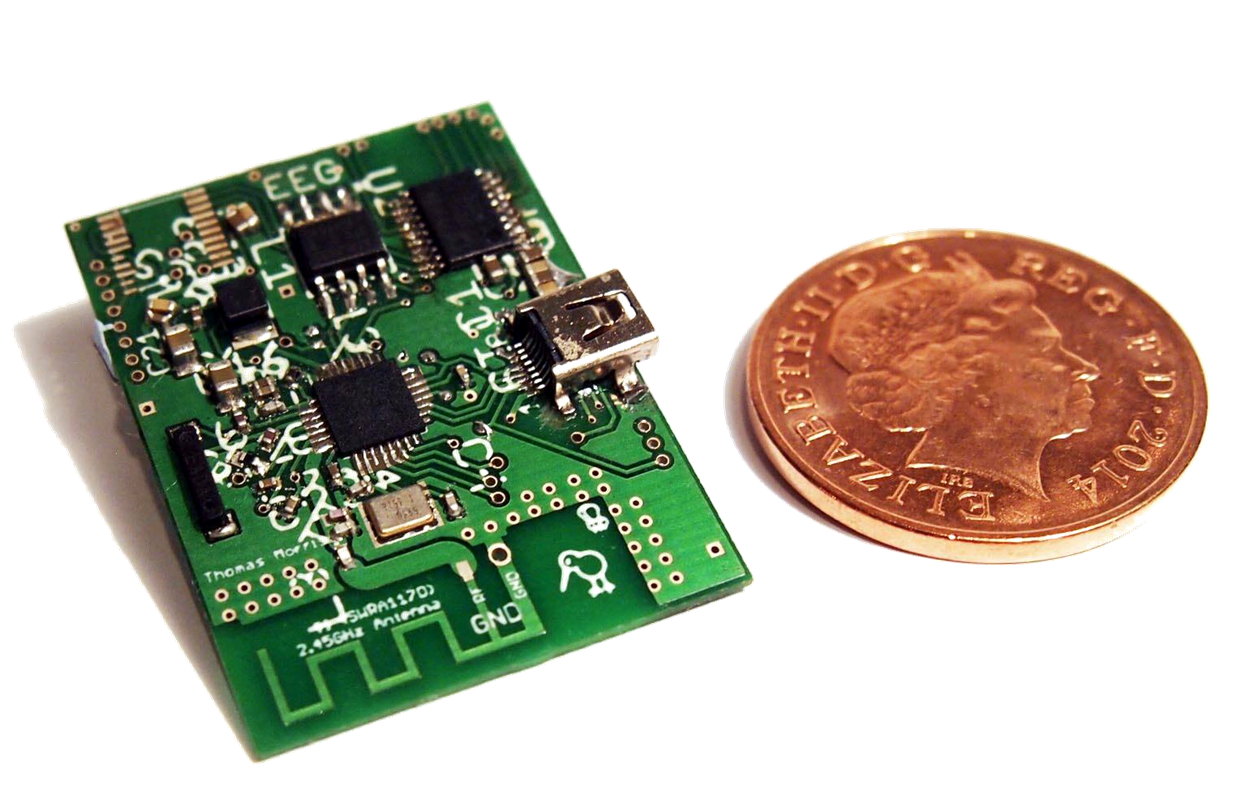
\includegraphics[width=0.9\columnwidth,keepaspectratio]{assets/front.png}

\vfill

\setlength{\tabcolsep}{0pt}
\begin{tabular}{p{40mm}p{\dimexpr\columnwidth-40mm}}
Project Title: & \textbf{A Wireless  Low Energy Ambulatory Electroencephalogram} \\[12pt]
Student: & \textbf{Thomas Alexander Morrison} \\[12pt]
CID: & \textbf{00642176} \\[12pt]
Course: & \textbf{EIE4} \\[12pt]
Project Supervisor: & \textbf{Dr. Esther Rodriguez-Villegas} \\[12pt]
Second Marker: & \textbf{Dr. Pantelis Georgiou} \\
\end{tabular}
\end{titlepage}

\clearpage





\clearpage

\section*{Abstract}
Certain neurological medical disorders require continuous monitoring to fully understand and diagnose. Examples of medical interest include epilepsy, syncope, multiple sclerosis, migraines, strokes, Parkinson’s and Alzheimer’s disease. \ac{EEG} is the recording of electrical activity along the scale, resulting from ionic current flows within the neurons of the brain and is useful for both diagnostic and monitoring such aforementioned conditions. Monitoring brain activity can help physicians understand certain characteristics, triggers, and the severity of the disorder. It may be possible to gauge the regions of the brain where the condition is originating and if the patient is a suitable candidate for treatment. 

However, symptoms from neurological disorders often appear sporadically and with little to no warning. Seizures vary from minutes to years apart, and sometimes are not realised or detected without proper equipment. Hospitalising patients for long periods of time is a costly option, and in such circumstances the patient could remain in hospital indefinitely.  Such circumstances lend themselves to an ambulatory system, where an outpatient can be monitored continuously without discomfort or hospitalisation, improving quality of life while decreasing costs. 

With the emergence of low power wireless technologies coupled with portable devices such as tablets and phones, it is a natural technological step to bring care and monitoring outside of the hospital. Through leveraging low energy radio capable platforms, i.e. smart phones and tablets, in the context of an \ac{AEEG}, it is possible to empower the patient to inexpensively take health care into their own home and out of the hospital. This project looks at maximising transmission of \ac{EEG} signals over the emerging wireless technology, \ac{BLE}. Further, while this project is targeted at \ac{EEG} signals, there is no reason why this research and technology cannot be applied to other signals and systems, examples including glucose monitoring, electrocardiography and spirometers.


\clearpage
\tableofcontents
\clearpage

\section{Acknowledgments}
\label{sec:Acknowledgments}
The opportunity is taken here to express gratitude to all those who have directly contributed towards the project. 

Firstly, the project supervisors, James Mardell, Chen Guangwei and Esther Rodriguez-Villegas from the Circuit and Systems departmental group, for the opportunity to undertake this piece of work along with my second marker for his efforts in reviewing this work. 

\ac{CSR} provided hardware and technical support in the spirit of academia. Particular acknowledgments go to employees Adam Hill, Martin Spikings, Mark Wade, Neil Stewart and Simon Finch. CSR have requested that this project report or relevant parts of it be made available to them.

Guan Yang and Jacob Rosenthal from New York, United States, for publicly making available a code source to drive nRF8001 radio. Imperial College student Stelius Ioakim for sharing experience of \ac{PCB} assembly. 

Dr. Nissim Zur, CEO of Vitelix Limited is an expert in low power wireless technologies, and has conversed over many aspects of the CSR1010 chip used. Further, he has also taken an interest in this project's work in regards to maximising the speed, and has requested the results be shared with him.

Special thanks go towards Mike Harbour and Victor Boddy for their efforts in printed circuit board manufacture and assembly. Countless hours were spent in the lab pushing the department's PCB fabrication facilities outside specification, assembling the boards and making debugging adjustments. It is unlikely this project would of been quite so successful without the help of level 1 laboratory staff. 

And finally, my girlfriend for her dainty and dexterous hands, along with her patience which was invaluable during circuit assembly. 




\clearpage
\section{Summary of Contributions}
This project has required a great deal of time and effort, drawing on a broad range of skills developed throughout my time at Imperial College. Achievements of the project are all my own work unless otherwise stated, and in no particular order are, current \ac{EEG} system evaluation and specification of a new system, hardware design (including RF), firmware design, high level software design, a full stack evaluation and a detailed academic throughput and power analysis. Within the tasks of programming there existed completely different mindsets and software paradigms. For example, when writing firmware, the paradigm is to be efficient with instructions and refrain from \ac{OOP} practices. This contrasts the high level programming mindset where abstractions and object management is seen as the way to model, implement and manage software solutions. Further, the first working (and smallest) \ac{PCB} board created for this project was done using the facilities on the departments first floor laboratories. The size and complexity of the board has received many positive comments, particularly as it was done outside the specifications of what the department is meant to be able to manufacture in house. 

This project has achieved beyond its original goal (and title) of "Maximising Bluetooth Low Energy throughput for \ac{EEG} signals", through designing and manufacturing a device to demonstrate the capabilities of \ac{BLE}, and hopefully be used for practical applications by Imperial College's circuit and system group. Finally, \ac{CSR}, the company which provisioned one of the development kits for the project has offered me a full time graduate position at their head office in Cambridge, United Kingdom.





\clearpage
\section{Introduction}

\subsection{Problem Landscape and Motivation}
Neurological disorders and their sequelae are estimated at present to affect upto one seventh of the world's population, a figure which currently stands at 1 billion. With the ever increasing life expectancy and decreasing (relative) fertility rates, the age demographic has shifted towards an aging population. This has caused a growth in neurological disorders such as Parkinson's, multiple sclerosis, Alzheimer's and other dementias. From the 2012 report published by the \ac{WHO}\cite{WorldHealthOrganization2012}, the societal costs of dementia for the United Kingdom totals £23 billion, a figure that matches the costs of cancer (£12 billion), heart disease (£8 billion) and stroke (£5 billion). Similarly a 2010 Swedish paper published that the costs of dementia (50 billion SEK) was higher than that of depression, strokes and alcohol abuse (32.5, 12.5, 21-30 billion SEK respectively)\cite{Wimo2010}. With neurological disorders constituting to approximately 12\% of the global mortality count\cite{WHO2006} and the expected increase in the number of cases and rising cost of health care, neurological disorders are an active area of medical research.

\ac{EEG}s are used extensively for detecting, characterising and monitoring brain activity related to the aforementioned diseases. Examples applications include diagnosing patients regularly loosing consciousness with syncopy; measuring the effectiveness of medication for patients currently diagnosed with epilepsy\cite{Duncan2006}; deciding whether the patient is a candidate for removal of the cortex part associated with the disorder\cite{Zijlmans2007}. Unfortunately many neurological disorder symptoms occur sporadically with little to no indication of an impending event, such as in the cause of epilepsy a seizure. In some circumstances the patient could remain in hospital indefinitely, however symptoms (e.g. seizures) can be seconds to years apart, and sometimes are not realised or detected without proper equipment. The diagnosis, monitoring and treating many of these diseases is currently a costly procedure due to the resource requirements (staff, time and equipment). Common practices include hospitalising and monitoring patients between 24 hours and a week.  Such circumstances lend themselves to an ambulatory system, where an outpatient can be monitored continuously without discomfort or hospitalisation, thus improving quality of life and social welfare (e.g. no sick days off work).

Since the arrival of \ac{BLE} in smart phones in 2012, the vast majority of smart phones are "Bluetooth Smart Ready" (incorporating \ac{BLE} technology). This is a relatively new technology capable of (very) low power communication for applications requiring a low data rate. This low power consumption means devices can have long lifetimes. While other low power wireless options exist such as ANT or ZigBee, \ac{BLE} is the only popular radio technology being manufactured into smart phones and tablet devices. In comparison, (classic) Bluetooth power consumption is typically 1 to 2 orders of magnitude higher than \ac{BLE}.

 Through leveraging widely popular and familiar smart phone devices with this new technology, in the context of an \ac{AEEG}, it is possible to empower the patient to inexpensively move their health care out of the hospital and into the home. By coupling cheap low power sensors and radios, with powerful ubiquitous consumer technology, it is possible not only to cheaply and efficiently monitor patients, improve the quality of life for patients but also help physicians further their understanding of neurological disorders. Further, when combined with data-mining or so called big-data analytics novel insights may reveal new understanding and ultimately better forms of treatment.


\subsection{Existing Research, Technologies and Products}

Over the recent past, reduction in power and size of technologies has enabled smaller and smarter devices, so much so, that they are known under the umbrella term as wearable devices. These wearable devices allow greater ease and lengths of monitoring  while barely impacting users in their day to day life. Hence, there has been and is a large amount of research in portable medical devices for health monitoring in both academia and industry. An investigation  into UK neurologist's reactions to wearable \ac{EEG} devices concluded that neurologists believe that wearable \ac{AEEG}s would be a major improvement in the \ac{EEG} practice for both patients and physicians, clearly signaling the desire for such systems \cite{asson2008}. This project and report is interested in investigating the use of \ac{BLE} as the wireless technology in wearable devices, specifically \ac{EEG}.

In academia, a 2010  paper reported a wireless 8 channel \ac{EEG} device capable of sampling 8 channels at 1024 Hz consumed an average of 12mW\cite{Brown2010}. The device used a custom \ac{ASIC} for measuring biopotentials with low power consumption and high frequency, and \ac{NS}'s nRF24L01 generic 2.4GHz transceiver for radio communication. In 2013, Washington University \cite{Dementyev2013} demonstrated a coin-sized 60 Hz sampling rate \ac{RFID} based system, which has unlimited battery life within the range of the \ac{RFID} transceiver.  While research papers are available discussing the use of \ac{BLE} for wearable devices and sensors \cite{Omre2010} \cite{MacKensen2012}, research on combining \ac{EEG} with \ac{BLE} is difficult to source (there have been many attempts published for \ac{ECG}, e.g. \cite{Yu2012}).

Currently, the Imperial College Circuit and System's group has a wired \ac{EEG} measurement device. The wired connection between the \ac{EEG} sensors and a fixed computer severely restricts patient's mobility and hence are impracticable for long periods of use. Figures~\ref{fig:imperialcurrent},~\ref{fig:eeghat} show the departments current immobile setup. 

\begin{figure}[H]
	\begin{center}
		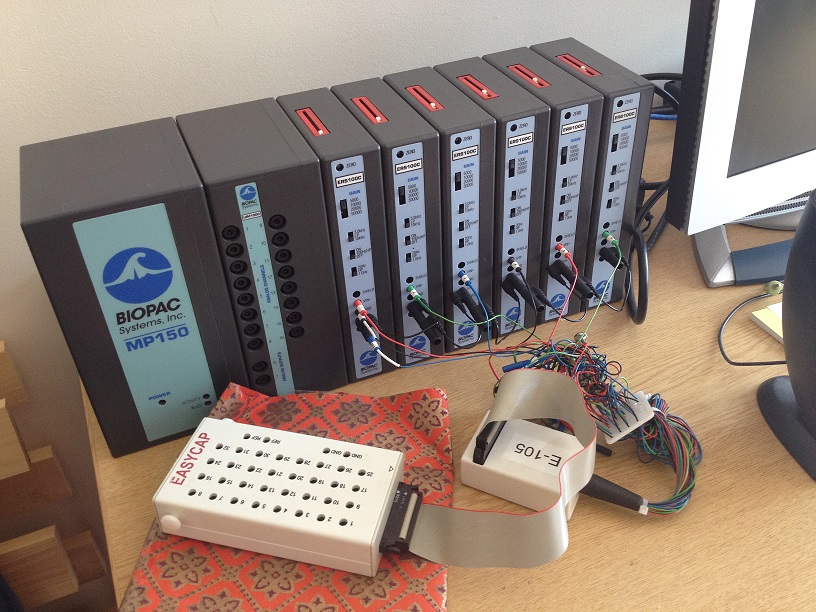
\includegraphics[width = 0.8\textwidth]{imperialcurrent}
	\end{center}
	\caption{Current \ac{EEG} setup at Imperial College}
	\label{fig:imperialcurrent}
\end{figure}

\begin{figure}[H]
	\begin{center}
		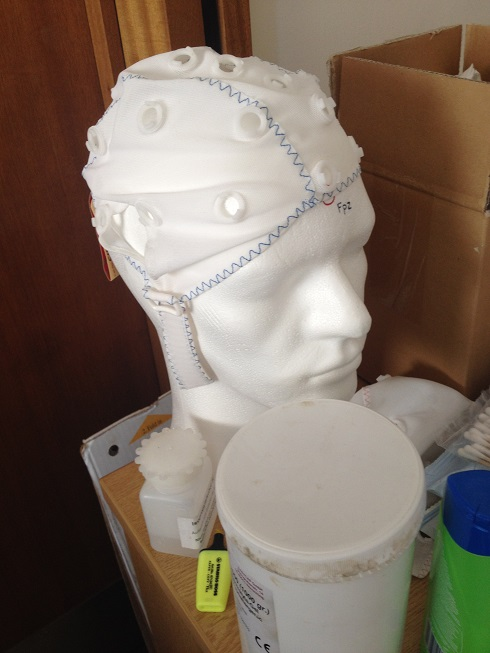
\includegraphics[width = 0.5\textwidth]{eeghat}
	\end{center}
	\caption{Example \ac{EEG} hat used by Imperial College}
	\label{fig:eeghat}
\end{figure}

Popular \ac{EEG} products on the market that have already shown integration with consumer electronics as well as research include Emotiv Systems' \ac{EEG} headset. The device retails at \$750 (approximately £450 at the time of writing), sporting 14 saline sensors, gyroscopes for positioning and a lithium battery capable of delivering up to 12 hours of continuous use.

\begin{figure}[htb]
	\begin{center}
		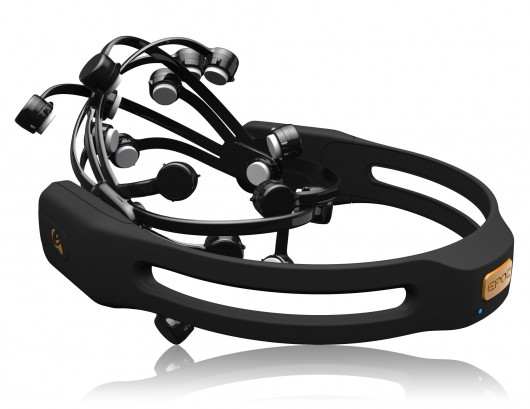
\includegraphics[width = 0.6\textwidth]{emotive}
	\end{center}
	\caption{Emotiv System's \ac{EEG} Neuroheadset}
	\label{fig:emotive}
\end{figure}

NeuroSky have released \ac{EEG} products, the MindWave and MindWave mobile. The foremost operates a proprietary radio system in the 2.4 GHz band, at a data rate of 250 kbit/s, a baud-rate of 57,600 and 10 meter range. It is also noted that there is a 5\% packet loss quoted on the device operation. The hardware samples at 512 Hz at a 12 bit ADC resolution. The device is powered from a standard AAA battery (1.5V), and has maximum power consumption of 50mW. The MindWave mobile uses Bluetooth and UART at the same baud rate of the previous, but the maximum power consumption increases to 120mW (80mA). Both devices weigh an equal 90g, and are priced at $80 and $130 respectively. 

\begin{figure}[H]
	\begin{center}
		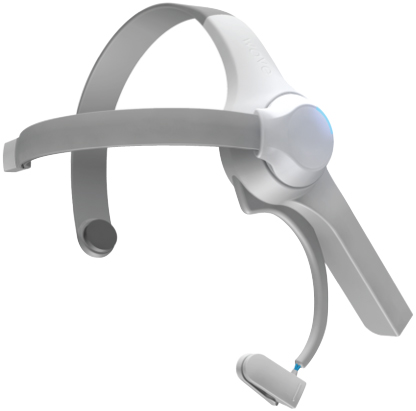
\includegraphics[width = 0.6\textwidth]{neurosky}
	\end{center}
	\caption{NeuroSky MindWave Mobile \ac{EEG}  Headset}
	\label{fig:neurosky}
\end{figure}

Away from specifically \ac{EEG}, the consumer fitness sector has been strongly targeted by wearable devices that can synchronise with a user's smart phone. At the time of writing many devices exist in the marketplace that utilise lower power technologies to act as gateways for real-time data logging. For example, there already exists a competitive market between heartbeat monitors, cadence monitors and pedometers. These ‘activity trackers’ use low power electronics and radios to log user's activities and update the user in real time with activity information through the user's phone or smart watch. Popular products on the market at the time of writing include the Fitbit, Fuelband and Jawbone, which all make use of the \ac{BLE} technology to connect to smart phones.

\subsection{Project End Goals}

 This project explores using \ac{BLE} technology for electroencephalography, having built a prototype system capable of interfacing with an analogue front to transmit \ac{EEG} data to a portable device such as a tablet or smart phone.  The report records the maximum throughput of such a device, the energy requirements and attempts to quantify the overall suitability of \ac{BLE} to \ac{EEG} monitoring.

In line with current \ac{EEG} practices and ideal requirements set forth by Imperial College's Circuit and Systems Group, the project attempts achieve at least the follow specifications
\begin{itemize}
	\item Running time of at least 12 hours
	\item Channel resolution of 8 bits 
	\item 16 channels
	\item A weight of less than 7 grams
	\item 10 meter range
	\item BLE wireless technology
	\item Ability to communicate with a smart phone or tablet
	\item Real time update of signals
\end{itemize}

\subsection {Structure}
The project is organised as the following. An overview of \ac{EEG} signals and \ac{BLE} technology is presented, giving background where it is believed relevant and of value to the rest of the project. It should be noted that these sections are not an exhaustive description of \ac{EEG} signals nor \ac{BLE}. The report will then move onto preliminary research, where the technology is evaluated and the components are discussed in detail (including risks) and a selection made for the prototype. A desired specifications is then presented from the components chosen.  The implementation section documents and discusses building, optimising and any issues found while developing the prototype. The results section lists the project findings, followed by a thorough evaluation of these results. A project wide conclusion can then be found where \ac{BLE}'s suitability for the application is discussed along with the limitations of the current system, and suggested future work for project extension or further interesting research as a result of this project. Lastly, a section is reserved for final remarks for comments that don't formally fit elsewhere into the report.

\clearpage
\section{Theory and Technology}
\subsection{Electroencephalography}

There already exists much literature on \ac{EEG} technology and archetypal signals measured (such as \cite{Teplan2002}), hence only a very brief overview is presented here. \ac{EEG} signals are detected along the scalp due to ionic current flow within the neurons of the brain. The typical bandwidth for signals is between 0.3Hz to 60Hz, with amplitude between 20-150$\mu$V, however more signals of higher frequencies may also be of interest \cite{Urrestarazu2006}. These signals can vary both temporally and spatially, and hence, multiple electrodes are positioned  around the scalp (typically in the standard international 10/20 format).

 The report is not concerned with the analogue front end for filtering and capturing signals, however digital conversion through sampling and providing sufficient resolution is of importance. The majority of signals are located below 100Hz, and hence, the expected normal use for this device will be 10 channels (as per the international standard) at 200 Hz. 


\subsection{Bluetooth Low Energy}
The original Bluetooth, here forth referred to as \ac{BTC}, was initially conceived as the solution to wired communication over short distances (typically less than 100m). The original specification had an air over-the-air rate of 1Mbps, though this has increased to around 3 Mbps in the latest version of \ac{BTC}. Similarly, BLE has an over-the-air rate of 1Mbps. Despite the odd realisation that \ac{BLE}, a much newer technology, has the same over the air rate of last the first incarnation of \ac{BTC}, the maximum theoretical throughput of \ac{BTC} is 700kBps, compared to less than 250kBps for \ac{BLE} - roughly one third of the maximum throughput \ac{BTC} was capable of (the latest version of \ac{BTC} brings the disparity to one ninth). While intuitively it may seem that \ac{BLE} is a less efficient technology, \ac{BLE} can be orders of magnitudes more efficient than \ac{BTC} in particular use cases.

Applications where \ac{BLE} excels  are ones where communication between two devices is only required intermittently, episodically and the volume of information sent is small. An example would be a thermometer in a greenhouse connected by radio to a visual display unit inside the home. Temperature changes at a rate slow enough that it is only necessary to check the temperature every 10 minutes. Once every 10 minutes the radio thermometer device can wake up take a measurement, send a notification of a measurement then return to a deep sleep. \ac{BLE} does this much better than \ac{BTC}, taking only a few milliseconds to connect. \ac{BTC} takes between a few hundred milliseconds to several seconds to reconnect. While both millisecond orders of magnitude and second orders of magnitude are small when compared to an order of magnitude of minutes, over time it adds up to a significant amount, and \ac{BLE} devices can last many years off a small, single coin cell. \ac{BLE} is excellent for applications which involve small episodic transmission of data. In the scenario described a \ac{BTC} system would have a lifetime of approximately 100 days from a typical 3V lithium cell. Off the same cell, a \ac{BLE} system would have a lifetime of many years. In fact, in this scenario the \ac{BLE} system lifetime can be extended further as \ac{BLE} can support connectionless communication, whereby it simply wakes up and transmits the thermometer state to any device that's listening without the need for acknowledgment. 

The reason the reconnection times are much faster for \ac{BLE} is as far as the communication devices are concerned, they never disconnected. Rather, in the \ac{BLE} protocol, the devices agree to meet a specified periods known as \ac{CI}. The devices are free to perform any operations in the mean time, though typically enter a state of hibernation. In many scenarios between two radios, one device will be much more power conscious. In the example above, the battery powered device in the greenhouse would typically be the power conscious device while the visual display unit inside the home will likely be powered from the grid, and have no concern as to its power consumption. In these situations, the power conscious device is defined to be the slave and the remaining device to be the master. 

The slave device also has the ability to skip connection intervals. That is, the slave to skip a up to a predetermined number of connection intervals, known as the slave latency. While the master must always check back to see if the slave has sent anything, the slave, if it has nothing to send, it doesn't need to wake up, conserving power. For example, if the slave latency is 120, and the connection interval is 1000ms, then the slave is not obliged to communicate with the master for upto 2 minutes, despite the master having to check every 1000ms. If the slave is not able to make contact with the master after 2 minutes, then the master will begin counting the number of times the slave has missed the obliged connection period (that is the \ac{CI} multiplied by the time slave latency). If this value reaches above a certain threshold (a typically recommended value of 6 times the slave latency), the master will consider the slave disconnected, and be required to go through a connection process again (unless using advertisements to send data as briefly mentioned previously). Continuing with the scenario, the slave will be considered disconnected if it hasn't made contact with the master after 12 minutes.

Another contribution to reduced power over \ac{BTC} is the reduction in the number of channels used in communicaton. \ac{BTC}, \ac{BLE} along with other wireless technologies that operate in the 2.4GHz ISM band such as a WiFi and ZigBee all make use of spread spectrum techniques to achieve a sufficient level of noise immunity. That is, the available bandwidth is split (spread) into smaller channels and radios communicate between one another using a pre-dertmined channel hop sequence. As the number of channels decreases, the channel band size grows requiring less accurate and complex modulation hardware, hence decreasing power consumption. \ac{BTC} originally used 79 channels, and \ac{BLE} reduces this to 39.

\begin{figure}[htb]
	\begin{center}
		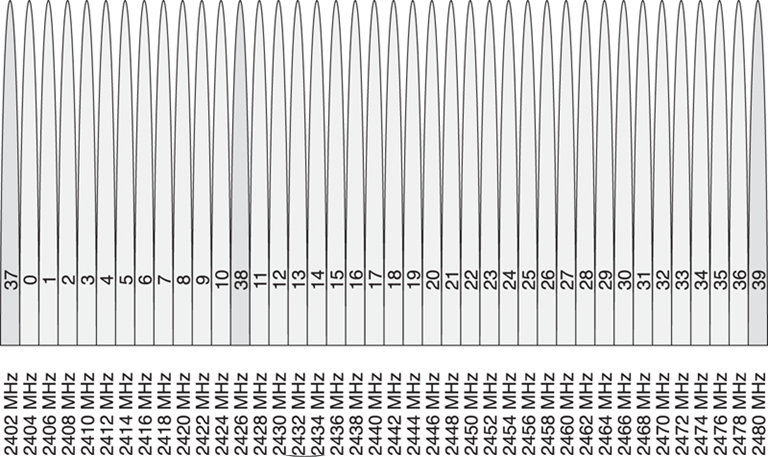
\includegraphics[width = 0.7\textwidth]{blechannels}
	\end{center}
	\caption{\ac{BLE} channels (advertisement channels render darker)}
	\label{fig:blechannels}
\end{figure}

\begin{figure}[htb]
	\begin{center}
		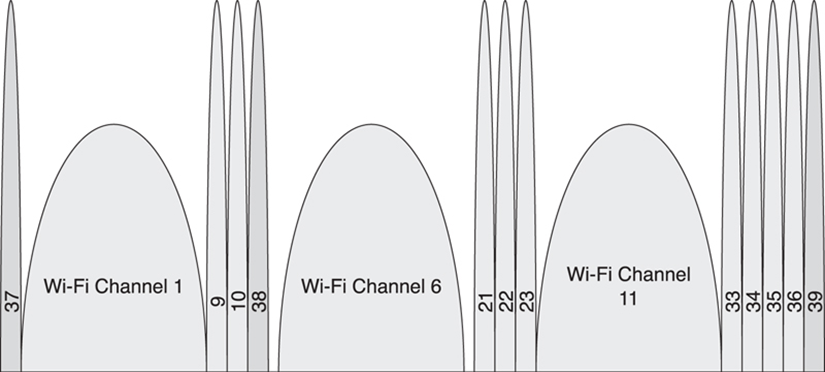
\includegraphics[width = 0.7\textwidth]{blechannelswifi}
	\end{center}
	\caption{\ac{BLE} channels with WiFi channels overlaid}
	\label{fig:blechannelswifi}
\end{figure}


The number of channels dedicated to advertising has also decreased, meaning less time is spent searching for discoverable devices. The advertisement channels have been specifically chosen not to interfere with the common WiFi channels. Finally, the radio characteristics are very dependent on temperature. Complex mechanisms are used to compensate and recalibrate on-the-fly radio parameters. Due to the episodic nature of \ac{BLE} the radio does not come under such thermal extremes. All these design changes have positive hardware ramifications. The reduced complexity of \ac{BLE} means reduced hardware requirements (notably memory), in turn reducing the leakage current. 

\ac{BTC} was designed with the idea that it would be used to do many common jobs, and hence particular configurations were built into it. In \ac{BTC}, these configurations are known as profiles. Example profiles include the audio distribution profile (A2DP), which is used in by many Bluetooth product manufacturers to allow a device, such as a phone to interact with an audio system, such as in a car. Another example would be the serial port profile (SPP), meant to emulate the highly popular and robust RS-232 serial standard for data transfer (recall that \ac{BTC} was conceived as a solution to wires). This is all built into what is known as the Bluetooth stack – a software framework that interacts between the physical layer and the application layer\footnote{Depending on what level of the stack one is working, master can take the names central or client, while slave can take peripheral or server.}.  

\ac{BLE} also makes use of this paradigm but is often superficially depicted as \ac{BTC} operating at lower speeds and power consumption. It is not currently compatible with \ac{BTC} and there are no plans for it to be. Like \ac{BTC}, the \ac{BLE} architecture has 3 over-arching parts: Application, Host and Controller. The controller, simply put, is the radio and related hardware controllers and the application the use case, which could be a cadence monitor, thermometer or even an electroencephalogram. It is the \ac{HCI}, commonly known as the “stack” that provides the necessary software to enable the application layer to communicate with the radio (see Figure~\ref{fig:ble_arch}).

\begin{figure}[htb]
	\begin{center}
		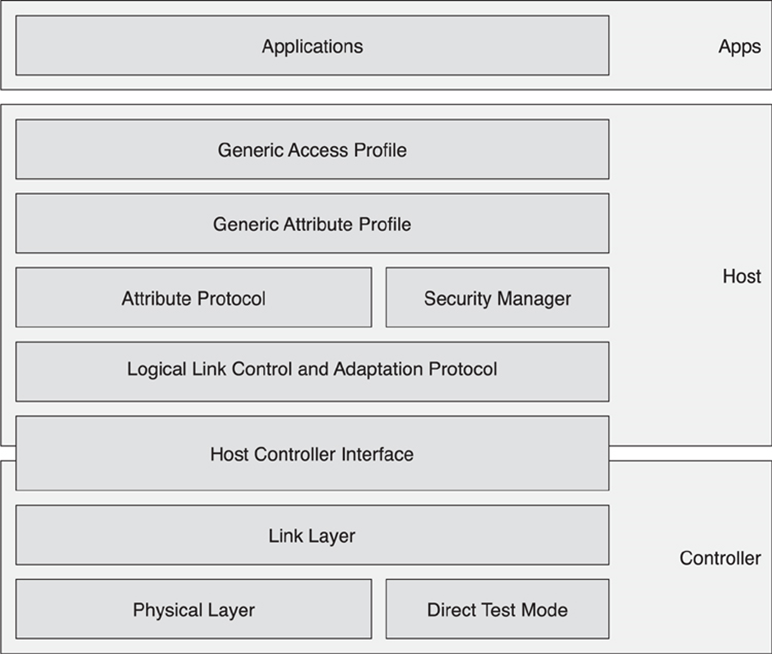
\includegraphics[width = 0.7\textwidth]{ble_arch}
	\end{center}
	\caption{\ac{BLE} Architecture}
	\label{fig:ble_arch}
\end{figure}

In an attempt to be economical with time and space, only components of the stack wholly relevant to the project will be covered in this report. Further information on areas not covered can be found in the \ac{SIG} specification website \cite{btspec}. For example a description of the security manager is not relevant as this project is not concerned with sending data over encrypted links. Similarly, the Logical Link Control and Adaption Protocol, while used extensively in all radio communication will not be discussed in detail as it doesn't provide any insight into maximising throughput or minimising power.

In \ac{BTC} profiles were diverse and large enough to warrant chip designers releasing tailored chips to perform well for a specific profile, i.e. a chip supporting A2DP may contain \ac{CODEC} hardware for real time audio streaming. In \ac{BLE} the profile framework is far lighter. \ac{BLE}'s profiles are all built on top of  the \ac{GATT}, which in turn is built upon the \ac{ATT}, a protocol optimised to run on BLE devices. Attributes are an umbrella term, being the atomic unit of (user) data communicated between BLE devices. Profiles are hierarchical constructions of attributes, in the top down order of profile, service, characteristic and descriptors, as shown in Figure~\ref{fig:exampleprofile}. A BLE device implements at least one profile, \ac{GAP} along one more which is typically the purpose of the device. \ac{GAP} contains important information such the the device name and preferred connection properties.  This second profile can be one of the standard profiles as defined by the SIG group or a bespoke profile for the application, such as the case for an \ac{EEG} sensor. Popular, SIG defined examples of \ac{BLE} profiles include the heart rate profile (HRP), health thermometer profile (HTP) and even a glucose profile (GLP) with room for many more to be incorporated into the core \ac{BLE} \ac{SIG} defined \ac{GATT} specifications.  

\begin{figure}[htb]
	\begin{center}
		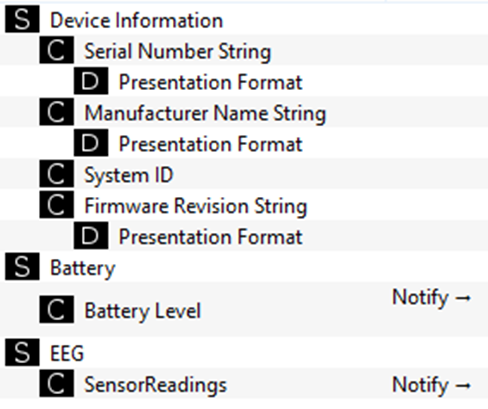
\includegraphics[width = 0.5\textwidth]{exampleprofile}
	\end{center}
	\caption{Example GATT profile consisting of 12 attribute - 3 services, 6 characteristics and 3 descriptors. }
	\label{fig:exampleprofile}
\end{figure}

 Attributes represent information about state. In the case of the greenhouse, the state would include the measured temperature. A suitable profile name which encapsulates the state is ''thermometer'', which contains the services ''device information'', ''battery service'', and ''thermometer''. As in figure~\ref{fig:exampleprofile}, the greenhouse thermometer service may contain the same device information and battery services, but replace the ''EEG'' service with the thermometer service, and the ''SensorReadings'' service with temperature. The other profile, \ac{GAP}, will contain the attributes which define how \ac{BLE} unit discover and establish connection to one another.  This includes the device name, perhaps ''greenhouse thermometer'', along with the preferred slave connection properties, e.g. a connection interval of 4 seconds, with a slave latency of 150 (10 minute window). All this information is contained within the GATT database, and shared as needed to other \ac{BLE} units. 

When communicating attributes, there are four operations available - read, write, indicate and notify. Read and write typically require one device to access the others characteristic. In the case of the greenhouse, the house device would request to read the thermometer. Notification and indications differ to read and write, in that the device(s) after information subscribe to the changes of state of the characteristics. For example, when greenhouse slave device wakes up, if the thermometer measurement changed, it will send a notification or indication alert the master device inside the house. The former methods can be thought of as synchronous means of communication while the latter asynchronous. Notifications differ from indications in that indications require a application level acknowledgment. That is, the indication is bubbled up to the user code, which then either accepts or rejects the indications. Notifications are acknowledge near the bottom of the \ac{BLE} stack, verifying correct receipt and message integrity. Therefore notifications are suitable for higher throughput applications. As shown in figure~\ref{fig:exampleprofile} shows notifications are operation configured for battery and EEG sensor readings. In this example, whenever the battery level changes, any devices subscribed to the characteristic battery level will receive a notification.

In \ac{BTC} the network topology used pico-nets, whereby one device has one master, but could be a master of another device. \ac{BLE} operates a simpler network topology, star, whereby a device can either be a master or slave, but not both. The master has the responsibility of organising itself between the slaves. If one slave requires large amounts of bandwidth, it my impact the quality of service encountered by the other devices. 

\begin{figure}[htb]
	\begin{center}
		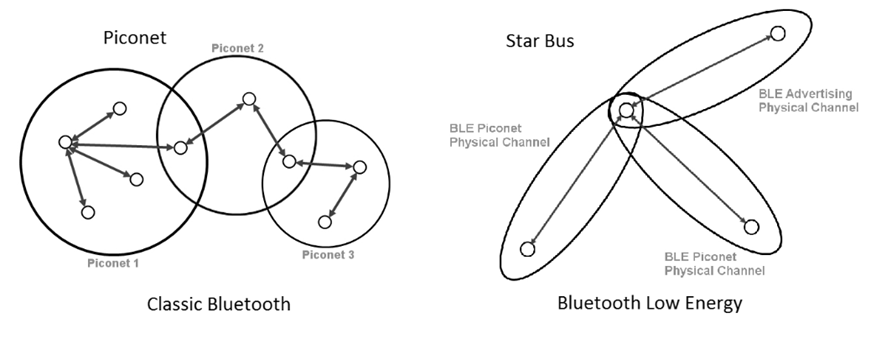
\includegraphics[width = \textwidth]{topology}
	\end{center}
	\caption{Bluetooth Network Topologies }
	\label{fig:topology}
\end{figure}

Both BLE and BTC devices move through generic system states. The same abstract view can be applied to both technologies and is shown in. Note that depending on the role of the device, the state moves right (master) or left (slave) from standby. It may appearing confusing to have another state for scanning which can only move into the standby state, but this is useful for searching and discovering devices with no commitment to connecting. Such a use case might be suitable for devices that intermittently broadcast small amounts of information. Assuming that the master BLE device is in the initiating state, searching for a connectible device, and at the same time the BLE slave is in the advertising stage, periodically broadcasting information using advertisement packets; the two devices will find one another and may initiate a connection request.

\begin{figure}[h]
	\begin{center}
		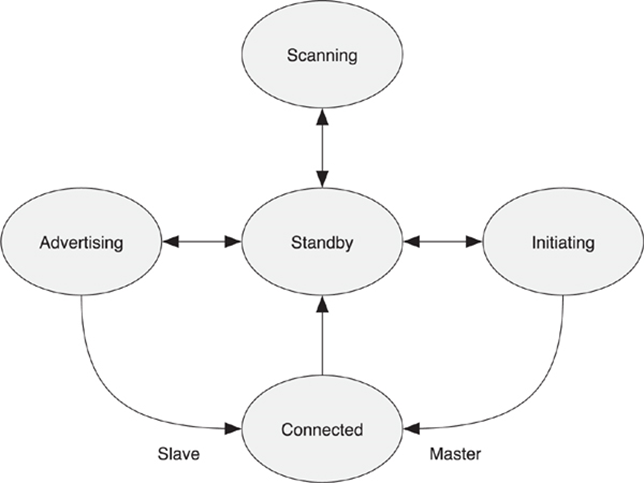
\includegraphics[width = 0.8\textwidth]{systemstate}
	\end{center}
	\caption{Device State Transition Diagram}
	\label{fig:systemstate}
\end{figure}

\ac{BLE} is principally composed of two types of packets, advertisement (Figure~\ref{fig:advertisement}) and data (Figure~\ref{fig:data}). Both packet types vary in length dependent on the payload but share a 32 bit advertising access address field, a 24 bit \ac{CRC} field, an 8 bit header and an 8 bit length field which defines the \ac{PDU} size (the last 2 field are often collectively called the header field). Advertisement \ac{PDU}s range from 0 to 29 bytes (232bits), meaning the total packet size can vary between 72 and 320 bits. The over-the-air data rate is 1Mbit/s, meaning advertisement packets are transmitted at a rate between 72 and 320$\mu$s (a single bit is transmitted every 1$\mu$s). In addition to the access code and \ac{CRC} fields, data packets consists of an 8 bit preamble and a \ac{PDU} varying between 0 and 27 bytes (4 of these bytes are reserved for encryption). Hence, the packet length varies from 80bits to 296 bits (328 including encryption). 

\begin{figure}[!h]
	\centering
	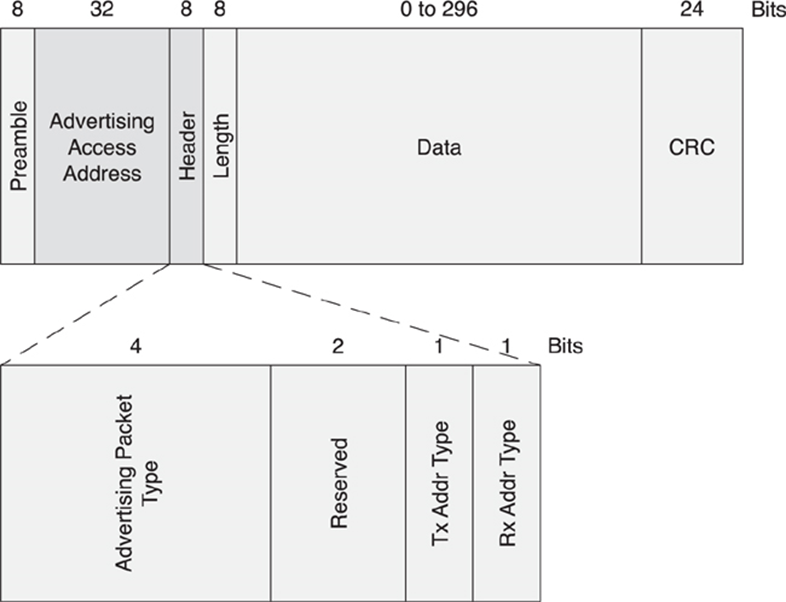
\includegraphics[width = 0.7\textwidth]{advertisement}
	\caption{\ac{BLE} Advertisement packet}
	\label{fig:advertisement}
	{Img advertisment}
\end{figure}

\begin{figure}[!h]
	\begin{center}
		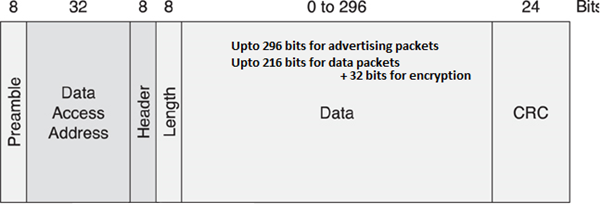
\includegraphics[width = 1\textwidth]{data}
	\end{center}
	\caption{\ac{BLE} Data packet}
	\label{fig:data}
\end{figure}

Figure~\ref{fig:connection} shows a connection between two devices being initiated. The first packet shown is is an indirect advertisement packet, available to all listening \ac{BLE} devices. The second packet is a connection request from the master device, communicating in the payload its address, the address to establish a connection with, and random access address, a connection interval length, the hop sequence, channel map, the connection timeout, slave latency and other things. Here the advertisement packets are rendered in green, the data in (predominantly) yellow (the magenta also represents a control data packet)
\begin{itemize}

 \item The channel map bit pattern corresponds to a contiguous stream of 37 ones, corresponding to all 37 channels being operational (the master has no reason to prevent transmission). 
 \item The hop byte indicates between each \ac{CE} how many channels the device pair will increment. From packet 242 onwards, the channel map increments every \ac{CI} (2 packets/30ms).
 \item The access address is a randomly chosen number (by the master) which acts as a identifier for a connection between two devices. 
 \item The interval of 0x18 (24 decimal) represents the \ac{CI} length in units of 1.25ms. Therefore 0x18 represents 30ms between subsequent \ac{CE}. Between each master to slave directional data packet (every 2 packets), the total sum of the time is 30000$\mu$s

\end{itemize}

It is highlighted that (at least initially) the slave interval is 0, meaning the slave should wake up every \ac{CE}. In packets numbers 243 and 244, the slave and master respectively have nothing to send, and simply acknowledge on another with an empty \ac{PDU}. The protocol realises flow control through the the lazy acknowledgment of \ac{SN} and \ac{NESN} bits, embedded into the header of every data channel.

\begin{figure}[!h]
	\begin{center}
		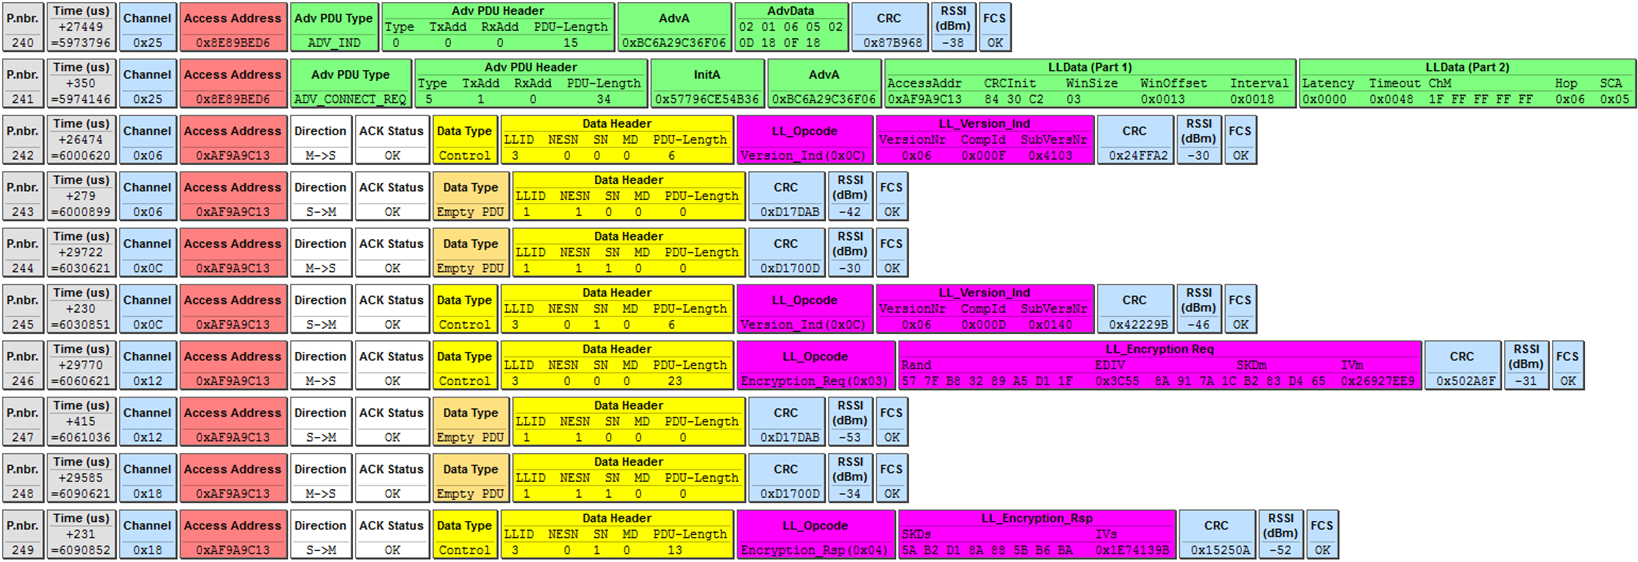
\includegraphics[width = 1.4\textwidth, angle=90]{connection}
	\end{center}
	\caption{\ac{BLE} connection initialisation}
	\label{fig:connection}
\end{figure}

While explained for completeness, advertisement and packets used in the initial establishment of a connection are of no concern to this project since they do not contribute to data throughput and once a connection has been established, do not contribute to the power consumption of the device. Hence, their contribution is removed from measurements as it is assumed the long term amortised cost is zero. The (incomplete) connection initialisation process shown in Figure~\ref{fig:connection} is known as "Just Works" pairing.



As previously mentioned, to achieve high throughputs notifications are used. To achieve the maximum throughput, it is desirable to send notifications as fast as possible. However, data cannot be sent out without flow control, and all notification packets must first be received then acknowledged before the next packet is sent. When a packet is sent, there is a mandatory 150$\mu$s inter-frame period. For the maximum throughput the connection receiving device would just acknowledge the data in an 80 bit acknowledgment response. Another 150$\mu$s frame would occur between this responding device and a transmitting device, bringing the total time up to:

\begin{displaymath}
296\mu s + 150\mu s + 80\mu s + 150\mu s = 676\mu s
\end{displaymath}

 This is shown graphically in Figure~\ref{fig:turnaround} (encryption is enabled). The maximum duty cycle is obtained when encryption is used 

\begin{displaymath}
\frac{328\mu s + 80\mu s}{708\mu s} \approx 55.6\%
\end{displaymath}
which is relatively low when compared radio technology duty cycles, e.g. \ac{BTC}. The 150$\mu$s inter frame period exists to prevents the silicon from heating to excessively, preventing power consuming hardware being required to recalibrate the radio. 

From the figure it is possible to calculate the upper bound for the number of packets that can be transmitted per second is

\begin{displaymath}\frac{1000000\mu s}{676\mu s} \approx  1479.29\;packets/second\end{displaymath}

Of the 37 bytes (296 bits) sent for a notification packet, 27 of them are known as the data payload. Even if encryption is not used, 4 bytes of the 27 are required for the L2CAP header use. The remaining 23 bytes are quoted as the available application bytes.

\begin{displaymath}
1479.29 \; \frac{packets}{s} \times 23 \times 8 bits \approx 270 kbp/s
\end{displaymath}

While many pieces of literate quote this 23 bytes as the maximum usable data rate, 3 bytes are required to identify the command type (notification) through an op-code (1 bytes) and  characteristic the notification belongs to through an attribute handle (2 bytes). This means that only 20 bytes of the original 27 reserved for the application are usable, reducing the upper bound for throughput to 

\begin{displaymath}
1479.29 \; \frac{packets}{s} \times 20 \times 8 bits \approx 236.7 kbp/s
\end{displaymath}

Here forth, the usable payload of a "notification" or "data packet" is 20 bytes. When aiming for either low power and/or high efficiency, it is important fill the usable payload with as much data as possible, as every notification packet sent has a fixed cost of 80 bits associated with it.  

\begin{figure}[h]
	\centering
		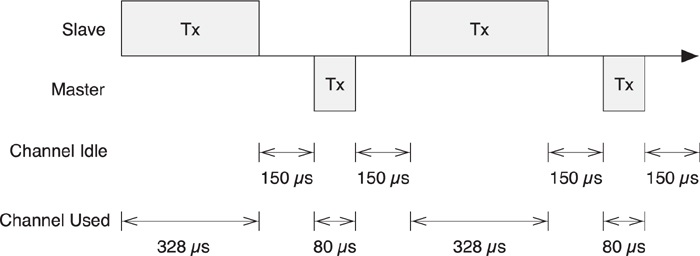
\includegraphics[width = 1\textwidth]{turnaround}
	\caption{\ac{BLE}'s packet flow for maximum throughput}
	\label{fig:turnaround}
\end{figure}

The \ac{BLE} protocol was not designed for high throughput applications, but rather for low latency episodic communication devices transferring small data payloads of representing device state. The energy per bit is low compared other popular technologies, and should not be used as the bottom-line metric for performance. Rather, a holistic measurement of the whole system energy consumption compared to a similar system is a more appropriate performance metric.








\clearpage

\section{Preliminary Research}

This chapter deals with evaluating the \ac{BLE} devices to choose a device most suitable for a maximising throughput and \ac{EEG} signals for an \ac{AEEG} system. This chapter goes on to evaluate and select \ac{AEEG} ancillary components required for the prototype.

\subsection{Radio Evaluation}

There are a number of competing companies int the \ac{BLE} consumer space. The most popular chip manufacturers at the time of evaluation are\ac{TI}, \ac{NS} and \ac{CSR}, although  other manufacturers exist, they normally design combo-wireless technology chips, e.g. Broadcomm, which only offers WiFi, \ac{BTC} and \ac{BLE} combined \ac{SoC}. These chips are not suitable for this project due to their complexity, packaging and intend application - the typical use case of such combo-chips are in high powered devices such as tablets, smart phones and notebooks. 

\ac{TI} provided an inexpensive \ac{BLE} packet sniffer which was used extensively throughout this project.

\begin{figure}[h]
	\begin{center}
		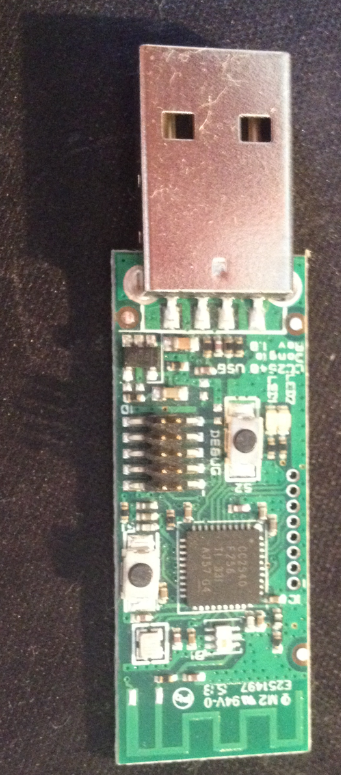
\includegraphics[width = 0.3\textwidth, angle = 90]{sniffer.png}
	\end{center}
	\caption{\ac{TI}'s \ac{BLE} packet sniffer }
	\label{fig:sniffer}
\end{figure}

As discussed in the previous section, to achieve the highest throughput values, the \ac{BLE} communication method used is notifications . Notification data packets can carry a usable payload of up to 20 bytes. The radio evaluation looks at selecting the best radio device that can achieve closest to the theoretical maximum.

%%%%%%%%%%%%%%%%%%%%%%%%%%
%%%%%%%%%%%%%%%%%%%%%%%%%%

\subsubsection{nRF8001}
The first radio tested was \ac{NS}'s nRF8001, selected due to the data sheet claiming it was the lowest power consuming device. The reason for this was because the chip only contained a controller and host layer. The application layer must be provided by an external micro controller, which is a large amount of effort to write. Fortunately a hobbyist open source project\cite{Guan2013} was available that provided the necessary code to get limited connectivity up and running. Figure~\ref{figure:nrf8001} shows the prototyping setup used to measure the performance of the nrf8001 microchip. 

Using a shunt resistor, the measured peak current was approximately 14.5mA, which correlates with the figure found in the data sheet (14.6mA). This was at a 

The ATMega328 consumes approximately XmA, however for the remainder. As the device was hardware limited to only 1 packet per connection event further development was abandoned.

\begin{figure}[h]
	\begin{center}
		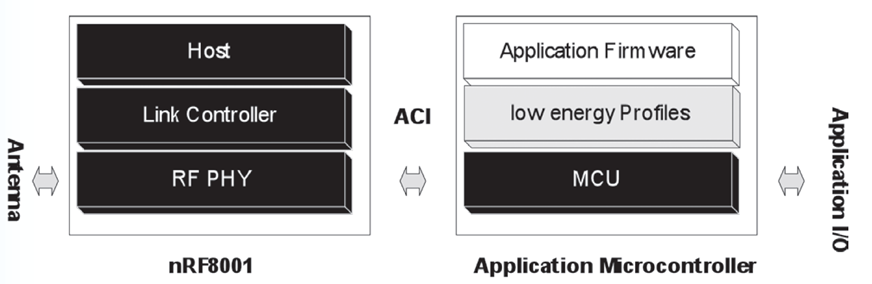
\includegraphics[width = 0.9\textwidth]{nrf8001stack}
	\end{center}
	\caption{nRF8001 application block diagram }
	\label{fig:nrf8001stack}
\end{figure}


\begin{figure}[H]
	\begin{center}
		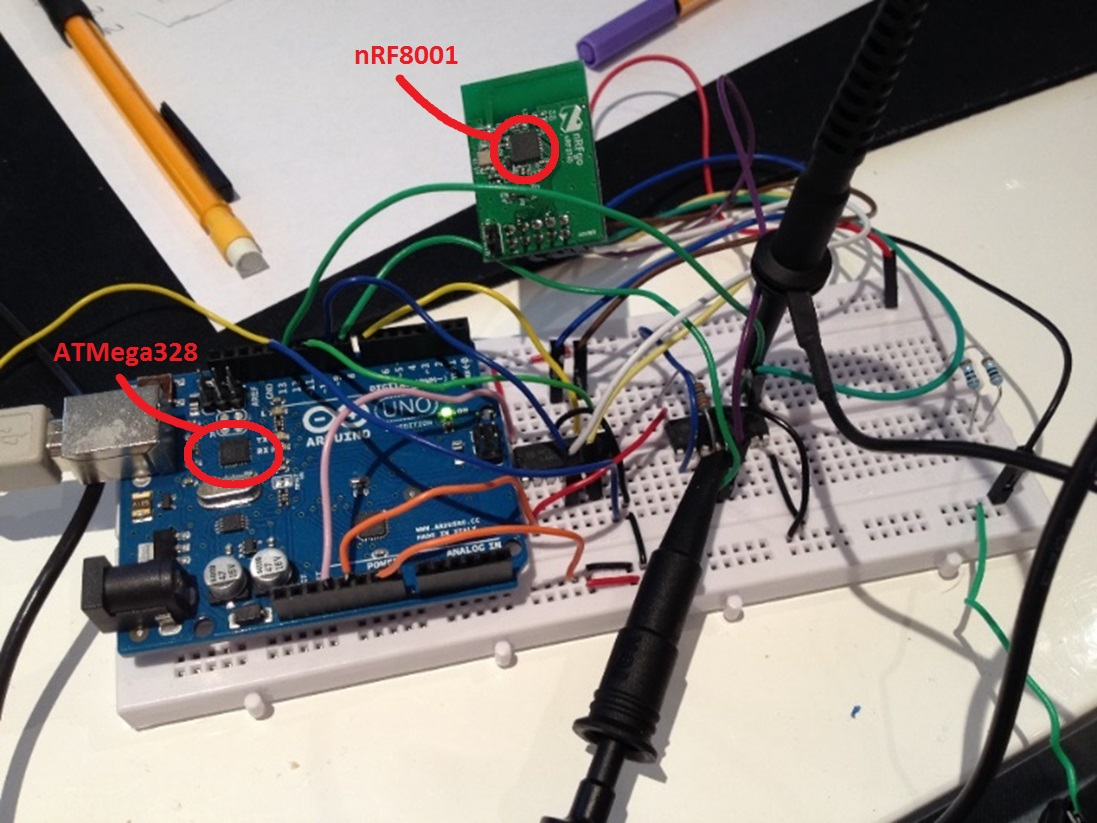
\includegraphics[width = 0.9\textwidth]{nrf8001}
	\end{center}
	\caption{Arduino Uno development board acting hosting the application layer for the nRF8001 radio. Level shifters were required for interfacing with the low-paper chip}
	\label{fig:nrf8001}
\end{figure}

\begin{figure}[H]
	\begin{center}
		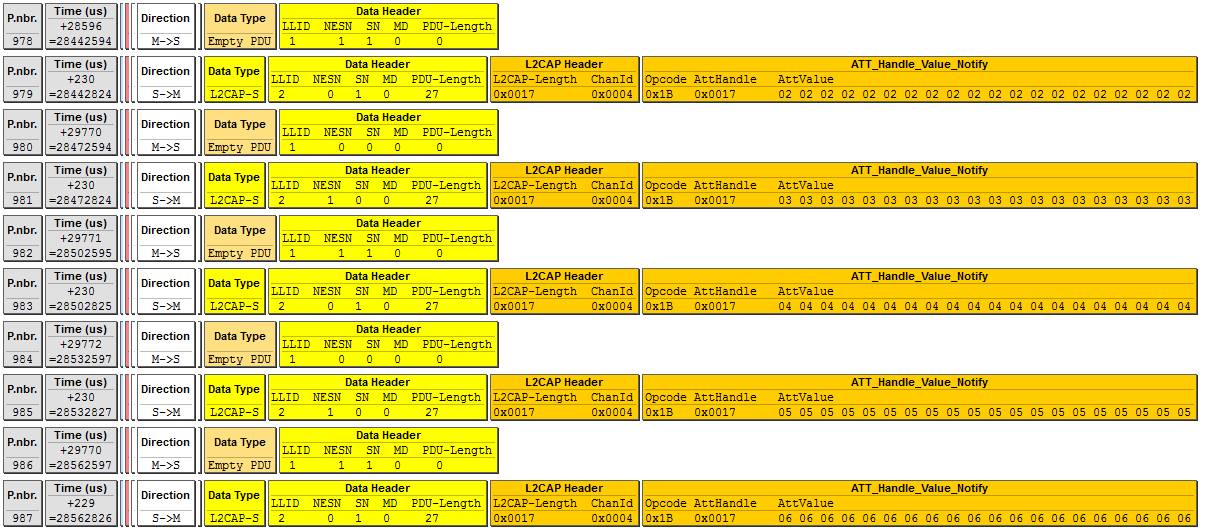
\includegraphics[width = 1.4\textwidth, angle=90]{nrfcap}
	\end{center}
	\caption{Packet-sniffed connection between Apple iPhone 4s and nrf8001. Notification rate 1 packet every 30ms. Some fields removed due to page space constraints}
	\label{fig:nrfcap}
\end{figure}

Initially, the device was configured to send a large amount of notification within a single \ac{CE} and at the lowest \ac{CI}. The master device was an Apple iPhone 4S, and it was found the total throughput was 5328 bit/s or 2.3\% of the theoretical upper bound. The reason for such a low throughput was two fold. Apple restricts the minimum \ac{CI} to 30ms through software (causing the slave \ac{CI} to increase. It has been reported this is due to issues with their design, whereby many radio technologies share the same antenna. 30ms is four times greater than the minimum \ac{CI} available. While this doesn't immediately reject throughput, longer connection intervals mean greater chance of a transmission error (CRC error), which if occurs, causes any further transmission within that \ac{CE} to case. The second reason, unlisted from the data sheet\cite{nrf8001}, is that the device is capable of only transmitting, on average, one packet per \ac{CE}. This is simply due to the hardware design, and ultimately believed to be why the device claims the lowest power out of all the radios. Figure~\ref{fig:nrfcap} shows a packet capture.


As the device can only send 1 packet per \ac{CI}, to achieve the highest throughput, the device must be run at the smallest connection interval of 7.5ms. At this interval the upper bound for throughput becomes

\begin{displaymath}
\frac{1000}{7.5} \times 20\:bytes \approx 2666\;byte/s
\end{displaymath}

With 16 channels at an 8 bit resolution, the highest frequency measurable (according to Nyquist condition) is 

\begin{displaymath}
\frac{1 2666\; byte/s}{16} \times \frac{1}{2} \approx 83  Hz
\end{displaymath}

A maximum support frequency running a solo channel is approximately 1328 Hz.

\subsubsection{nRF51822}
Another \ac{NS} product tested was the nRF51822. Information on the suppport packets per connection event was also not present in the data sheet\cite{nrf51822}. This device was found capable of receiving up to 6 packets per second, and this was verified by an engineer\cite{olme}. While a marked improvement over the nRF8001, this meant that the device was only capable of operating at 60\% of the maximum throughput capable as claimed in the specification. The maximum support frequency per channel for 16 channels at 8 bits resolution is 500Hz.

\clearpage

\subsubsection{CSR1010}
\ac{CSR} provided the CSR1010 development kit consisting of a basic board containing a CSR1010 radio chip, a programmer (USB to \ac{SPI}) and  a \ac{BLE} capable dongle (Figure~\ref{fig:csrdevkit}). 

\begin{figure}[H]
	\begin{center}
		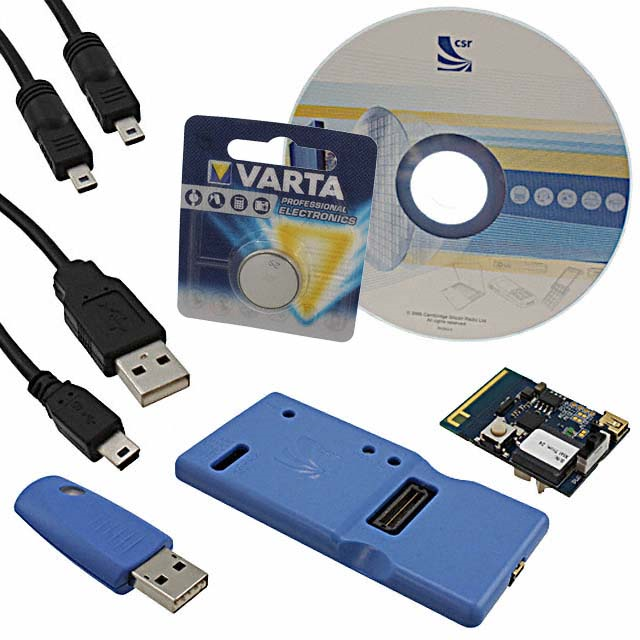
\includegraphics[width = 0.8\textwidth]{csrdevkit}
	\end{center}
	\caption{CSR1010 development kit (image from DigiKey.com)}
	\label{fig:csrdevkit}
\end{figure}

Through direct contact with \ac{CSR} engineers, it was reported a particular single mode \ac{BLE} radio device, the CSR1010, was measured reaching 250kbps

\begin{quote}\itshape \ldots the theoretical maximum throughput for a single BLE 
connection using a much bandwidth as possible is around 300kbps at the 
air interface. The usable application data rate is somewhat less, but 
80kbps should be possible (Using ATT packets with a 23-byte MTU should 
provide approximately 200kbps application data rate, if my maths is 
correct).

However, in practise you are limited by what other activities each end 
of the link is doing. In particular smart-phones (as one end of the BLE 
link) will likely severely restrict the BLE throughput to account for 
other Bluetooth activities (such as eSCO links) and co-existence with 
WiFi etc. But if you controller both ends of the link (e.g. single-mode 
BLE devices at both ends) then it should be easier to get close to the 
maximum theoretical rate.  \text{ \textnormal{[sic]}}
\end{quote}[sic]

 In the first paragraph the engineer is treating the full 27 bytes in the data payload as the application data. This number should of come from

\begin{displaymath}
\frac{1000000 \mu s}{676 \mu s} \times 27 < 320 kbps
\end{displaymath}

320 to 300 is a generous approximation, it is believed that the engineer actually rounded a smaller number, 305, which was calculated by including an unnecessary 32 bit \ac{MIC}, used only when encryption is enabled

\begin{displaymath}
\frac{1000000 \mu s}{708 \mu s} \times 27 \approx 305 kbps \approx 300 kbps
\end{displaymath}

Many literature pieces and training materials on \ac{BLE} make this assumption, including those on the \ac{SIG} website \cite{sig} \cite{sigdebug}. 

In the second paragraph the engineer is highlighting some important facets of \ac{BLE} devices, and that is the data rate of the link is determined by the lower of the two device's throughputs. The engineer cites smart phones as such devices that restrict the link capability. This was seen in the nRF8001 - the iPhone 4S could not handle a connection interval less than 30ms. Combined with that the nRF8001 stack couldn't transmit more than one packet per connection interval on average, the maximum throughput achievable by this device was cut by 4. 

When asked how to show the math behind the numbers achieved

\begin{quote}\itshape

While testing our uEnergy silicon (CSR1010) at HCI level I can achieve 
~250kbps throughput using a dedicated test application (i.e. data 
generated on-chip). HCI packets are 27 bytes, so to get my earlier 
number I simply did (20/27) * 250 to get an application-level data rate 
(27 bytes minus 4 bytes L2CAP header minus 3 bytes ATT header, leaving 
20 bytes for application in each packet).

I haven't tested raw throughput at the application level, but as our ATT 
protocol runs on stack alongside the HCI/controlller level, it should 
not see any additional processing overheads. \text{ \textnormal{[sic]}}

\end{quote}

The \ac{HCI} is the component between the host and controller layers shown in Figure~\ref{fig:ble_arch}. The engineer is saying that data throughput should no be affected by any high-level stack activity (any stack congestion, if existing, shouldn't affect throughput). Although the engineer has given no comment on latency (data will take time to propagate up the stack).

 \ac{CSR} supplied a development kit consisting of  provided a development board (CNS10004V5D) and \ac{USB} dongle. The CSR1010 is part of \ac{CSR} 's new $\mu$Energy product line, for which \ac{CSR} have developed their own compiler and \ac{IDE} known as xIDE. For initial throughput testing, an example health thermometer application was used. From exploring and understanding the main features of the \ac{OSAL}, it was immediately possible to increase the number of notification packets sent per connection interval from 1 to 8. 

The standard mechanism provided in the example, is for every connection interval a confirmation of the first acknowledge is raised in the application layer. This is used in the program as a point of reference for application layer timers, so schedule the next wake up time, etc.  This mechanism provides visibility at the \ac{CE} level, but not at the notification packet level - if many notifications are sent and acknowledged, this method doesn't provide any information that the \ac{CE} may have room for more notifications. This is a problem when large throughputs are desired, as it appears the buffer queue is 8 packets in size. When more than 8 are added to the queue, they are ignored, causing data loss. Hence, through the naive method, whereby notifications are placed into the queue before or after the start of the \ac{CE}, up to a maximum of 8 notifications are correctly sent in order. While it is possible to continuously flood the stack (buffer queues) with more notification requests, without knowing if the stack is capable of dealing with them, data may be lost. This mechanism is visualised in Figure~\ref{fig:nols}. 

\begin{figure}[H]
	\begin{center}
		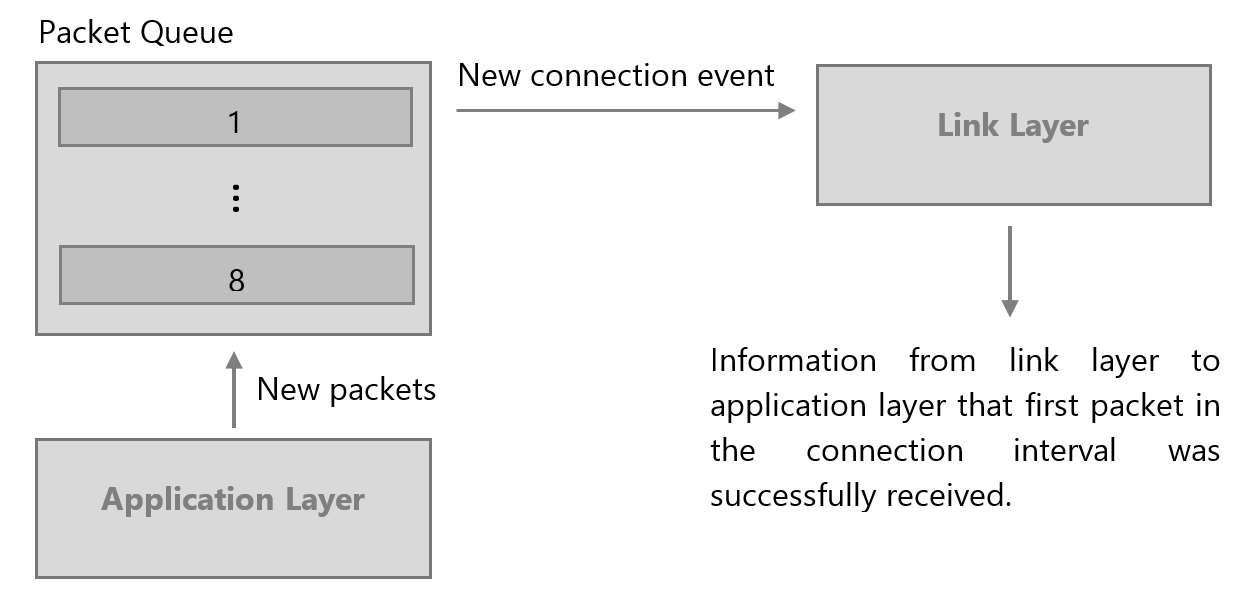
\includegraphics[width = \textwidth]{nols}
	\end{center}
	\caption{Notification of the first packet}
	\label{fig:nols}
\end{figure}

An experiment to test throughput was setup whereby each connection event sends 8 notifications per connection event with the same payload, bar one byte which increments with the connection event. The output can be seen in Figure~\ref{fig:8pckt}.

\begin{figure}[H]
	\begin{center}
		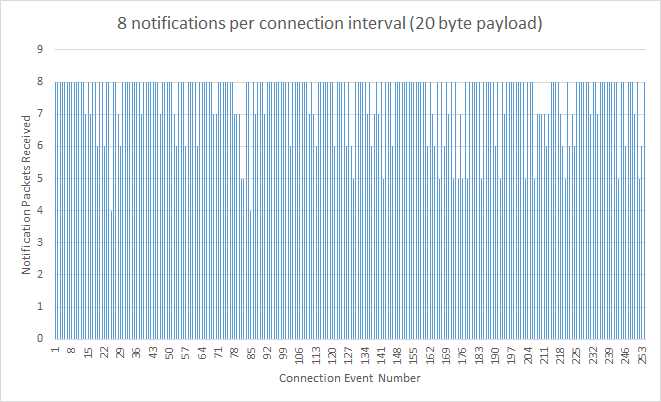
\includegraphics[width = 0.8\textwidth]{8pckt}
	\end{center}
	\caption{Queuing of 8 packets being lost}
	\label{fig:8pckt}
\end{figure}

From the experiment above, the conclusion was that the link layer stack became flooded with notification requests. Had the requests been accepted into the stack, then they would of been transmitted. If they failed to arrive at their destination, then the flow would of caused a negative acknowledgment, and the packet would of been retransmitted. Provided the notification made it through the link layer stack, it should appear in the output. 

After greater exploration of the software system framework, the \ac{API} and software mechanisms, it's possible use the message pump to signal whenever a packet is acknowledged. Upon receiving this signal, the device can then dispatch a subsequent packet. Figure~\ref{fig:lsrad} shows such a mechanism. 

\begin{figure}[!h]
	\begin{center}
		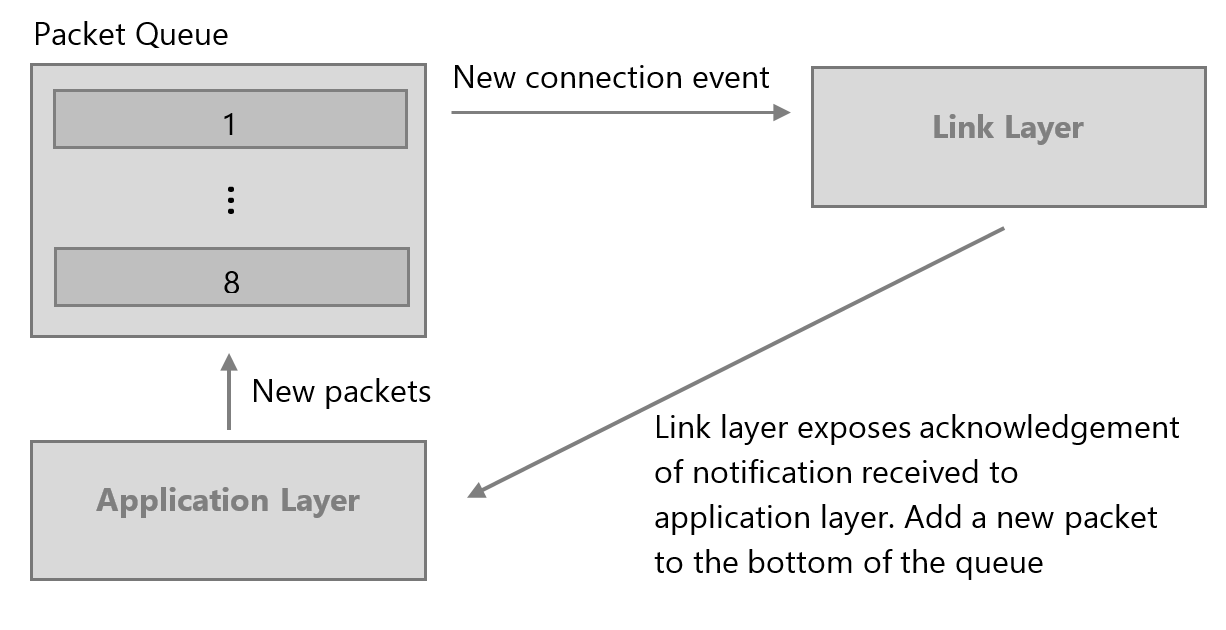
\includegraphics[width = \textwidth]{lsrad}
	\end{center}
	\caption{Upon packet acknowledgment }
	\label{fig:lsrad}
\end{figure}

The experiment was repeated again, this time sending a new notification every time the previous one was acknowledged using the message pump signal. The results are shown in Figure~\ref{fig:9pckt}

\begin{figure}[!h]
	\begin{center}
		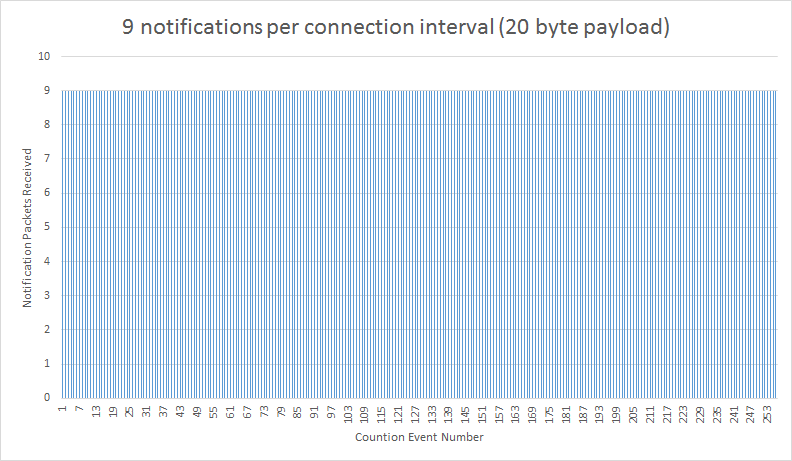
\includegraphics[width = \textwidth]{9pckt}
	\end{center}
	\caption{9 packets being received per connection interval when through acknowledgment feedback mechanism}
	\label{fig:9pckt}
\end{figure}
 
A capture of the notification data was taken over a period of approximately 46 seconds. Figure~\ref{fig:wireshark} shows part of the capture. 

\begin{figure}[h]
	\begin{center}
		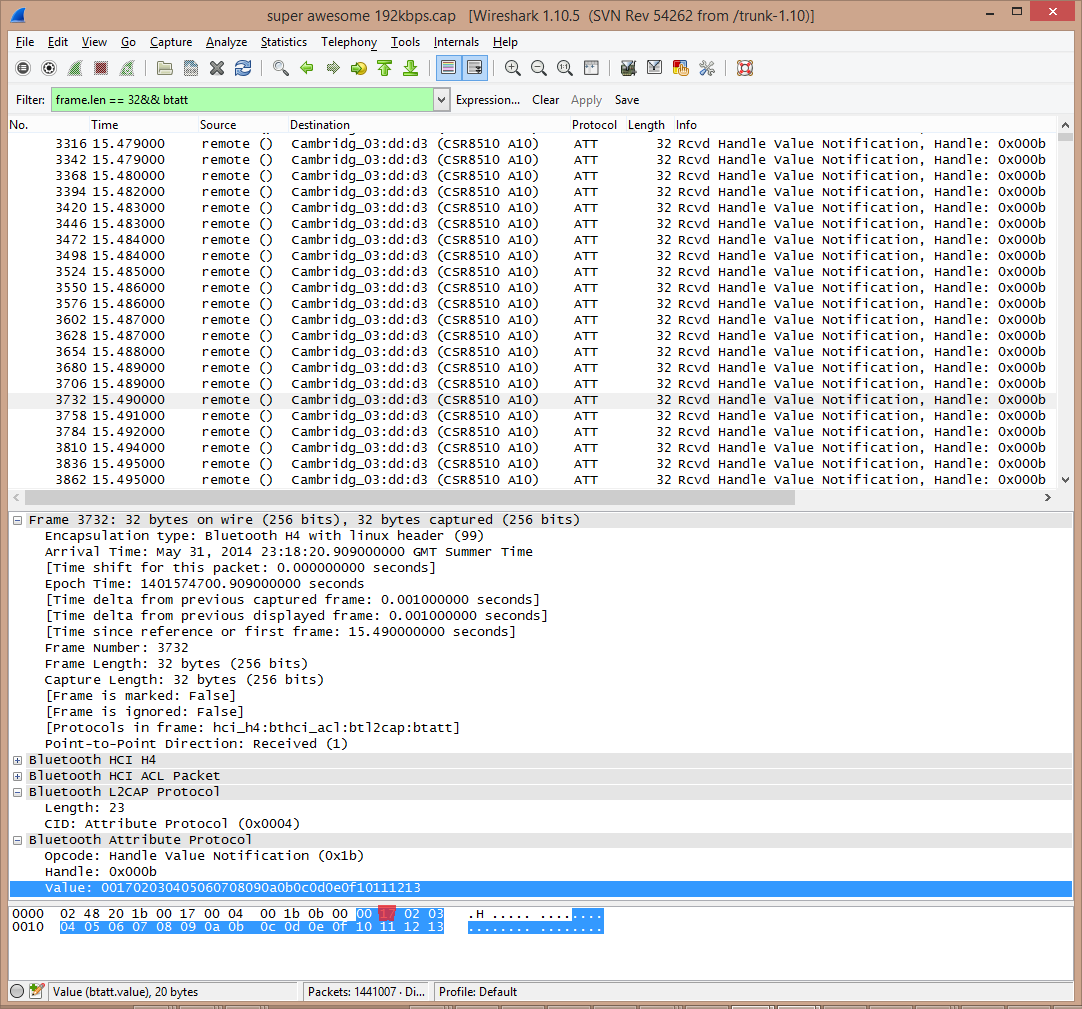
\includegraphics[width = \textwidth]{wireshark}
	\end{center}
	\caption{Packet capture. 20 byte data payload (blue) and connection event counter variable highlighted (red). Resolution of time stamps is to the nearest millisecond}
	\label{fig:wireshark}
\end{figure}

In the 46.060 second period a total of 55286 notification packets were captured, bringing the average throughput to


\begin{displaymath}
\frac{55286}{46.060} = 1200.30395137\; packets/s
\end{displaymath}

For the 7.5ms \ac{CI} used, the number of \ac{CE} is 133.333 and the number of packets per connection interval is

\begin{displaymath}
\frac{1200.30395137}{133.3333} = 9.0027\; packets/s
\end{displaymath}

Therefore 9 packets per connection interval at 7.5ms. This corresponding to a throughput of 192kbps or over 80\% of the theoretical maximum. A comprehensive explanation of the code used to achieved this is provided in the later section \ref{Implementation}. 

\clearpage
\subsubsection{CC2540 and CC2541}
\ac{TI}'s CC2541 is part of the sensor tag package - a \ac{BLE} one of the first and most popular development kits. The CC2540 differs in that it's range and power usage are increased, though it's throughput is theoretically the same.

\begin{figure}[H]
	\begin{center}
		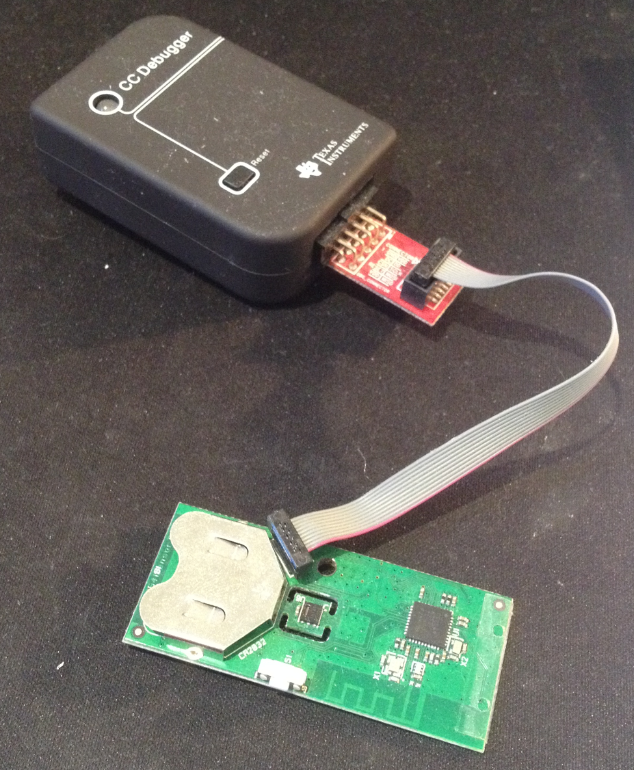
\includegraphics[width = \textwidth]{sensortag}
	\end{center}
	\caption{SensorTag hardware (contains CC2541) and programmer}
	\label{fig:sensortag}
\end{figure}

Again, the associated white papers did not document the packet throughput per \ac{CE}. Through contact with a \ac{TI} employee \cite{tiem}, there is a hardware limitation of 4 buffers, limiting only 4 packets per \ac{CE} (each buffer contains 1 packet). Each buffer is 128 bytes in length, while \ac{BLE} data packets can be a maximum of 41 bytes. Through using an exposed firmware (software) switch it was possible to increase the throughput slightly to achieve 5 packets per\ac{CE} by refilling the buffers within the \ac{CE}, once the packet has been link layer acknowledged. Again, this was discovered through a Texas instrument employee. This increased the average packets per \ac{CE} to approximately 4.6, bringing the total throughput between 10-12.3k byte/s.

The CC2541 (and also CC2540) is a full \ac{SoC} - a programmable \ac{MCU} is packages together with the radio hardware. This has certain economical advantages, as common hardware and footprint is shared between the radio and \ac{MCU}. However, the Nordic company Chipcon who originally developed the hardware (Texas Instruments has since acquired them), relied on the Swedish tool chain provider, IAR, for the development tool suite and chain. \ac{TI} still relies up this tool software suite, haven't not invested in their own facilities to develop for the platform. A single software license is approximately 2000 USD. While IAR do offer a code-limited version, it is too small to contain all the necessary libraries. IAR also provide a 30 day trail, which is what is currently being used for evaluation, but proceeding with this chip for the prototype may be economically impossible.

For the measured packet throughput, for 16 channels running simultaneously, at 8 bit resolution, the highest achievable detectable frequency is approximately 384 Hz.

The observant reader may notice that the \ac{BLE} sniffer from \ac{TI} is actually the CC2540 chip, which is reported as limited to between 4 and 5 packets per \ac{CE}. However, when loaded with the firmware as a sniffer, it is capable of sniffing many more packets than this. After contacting a \ac{TI} employee about this disparity, they reported that the sniffer uses a completely different stack:

\begin{quote}\itshape The sniffer is capable of listening to any number of packets during a single connection event. Note that the CC254x sniffer SW is completely different than the CC254x stack.\end{quote}

 The engineer highlights that the software used on the sniffer is completely different than that used on the normal CC254x stack - this is presumably means the sniffer runs a reduced/highly specific operating system, to reduce overheads associated with a more generic system. This may mean the hardware is capable of sending large numbers of notifications per \ac{CE} but either no supporting firmware or a ac{MCU} powerful enough can drive the chip to these operational levels. 

\subsection{Batteries}
There are many different battery technologies available. For the device a small, low profile low footprint, a lightweight battery is required. Given that \ac{BLE} can consume upto 15mA at peak current draw, taking this as the upper bound means that for 12 hours of continuous use batteries with capacities of 180mAh should be considered. Although the radio will dominate, other parts of the circuit such as the Microprocessor will consume a small amount of power, so this figure is arbitrarily upped to 200mAh. Note that peak current is an unfair way to measure current consumption in \ac{BLE}, however it is being used here as a worst case scenario. 

Two batteries technologies which satisfy these requirements are Lithium-ion (the popular CR2032 is typically advertised as an energy source with many \ac{BLE} modules) or Zinc-air batteries with capacities of 600mAh cheaply available. Common voltages are 1.4V to 1.65V (radios require between 1.8 -3.6V). However the batteries are light, less than 2g each (one CR2032 weighs, on average, over 3g), therefore they can be combined in series to provide a suitable voltage and a large capacity (over 1Ah). Further, this high voltage will allow the effective radio range of the \ac{BLE} device to increase. If a Zinc-air cell exhibits damage, unlike most technologies, no dangerous chemicals are present. The downside to zinc-air batteries is that they must be vented to an oxygen environment (cannot be hermetically sealed) which in turn causes them to lose their charge over time relatively quick once exposed to air. Although the \ac{AEEG} use case requirements will require the device to have lifetime of hours to days, not years. 

Two Zinc-air batteries weighing in at 1.9g each, can supply over 1000mAh with a combined series voltage of 2.8V. In the worst case of BLE drawing 15mA, the battery lifetime is approximately 3 days. Recall 15mA is the peak current and BLE will never continuously draw this current, hence the lifetime of the device should be greater, depending on the throughput. ac{BLE} was designed that current is never continuously consumed, and between radio events, the battery has recovery periods, extending the useful life of the battery.

\ac{NS} provides a battery lifetime calculator. Using a typical Lithium-Ion battery of 220mAh at a 7.5ms connection interval, yields a lifetime of ~163hours. This makes sense as the current average current consumption is slightly above 1.3mA and the capacity of the battery is 220mA. Accuracy of this model will be verified in the power analysis of the \ac{AEEG}, but the simulation looks sensible. Figure~\ref{fig:nrfsim} shows a notification simulation of the EEG service being sent continuously every 7.5ms. This model is only for 1 notification per connection event. 

\begin{displaymath}
\frac{7.5ms}{0.676ms} = 11.094\; notification\; packets\; per\; conneciton\; interval
\end{displaymath}

\begin{displaymath}
\;
\frac{163 \;hours \;for \;1 \;notification\; per\; connection\; interval}{11.094 packets per connection interval} \approx 14.7 hours
\end{displaymath}


This should be an overestimation of the power requirements, as there is a fixed cost payed for waking the MCU, which would be amortised for higher throughputs. Further in the model above the idle time contributes to the power consumption, but at full throughput, there will be little idle time. Finally, running at full throughput is not necessarily the end used case. Running at lesser throughputs will have a dramatic effect on the power consumption.
 

\begin{figure}[htb]
	\begin{center}
		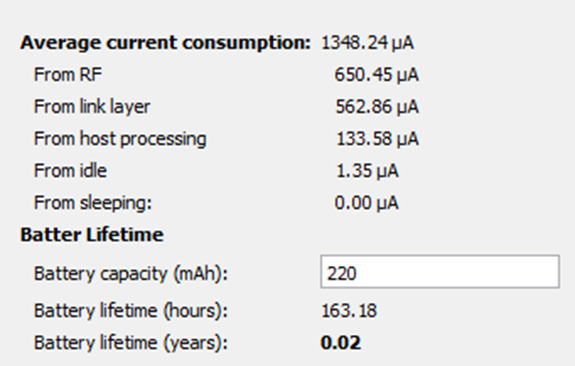
\includegraphics[width = 0.5\textwidth]{nrfsim}
	\end{center}
	\caption{Power consumption and lifetime calculator}
	\label{fig:nrfsim}
\end{figure}

\begin{figure}[htb]
	\begin{center}
		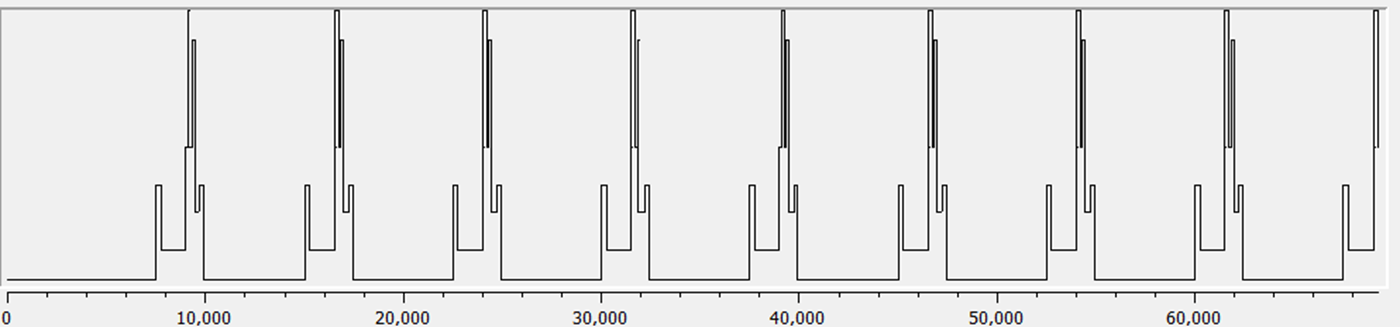
\includegraphics[width = 1.1\textwidth]{nrfwave}
	\end{center}
	\caption{nRF8001 waveform (1 transmission per connection event}
	\label{fig:nrfwave}
\end{figure}

 
Figure 23 - Simulation plot of notifications being sent
For 2 zinc-air batteries of 500mAh capacities, this model predicts the device lifetime under nominal operation begins to reach 10 days.  An intelligent estimate to how this module is generated is linked to the throughputs calculated at the start of the Radios section. As each bit represents 1 micro second it is very easy to integrate for set parameters the time over time the current profiles to achieve an estimate of power usage. 
Max drain current is another important concept to consider. Batteries can only safely deliver a maximum amount of current. If the battery is stressed to deliver more current that it is rated, it will degrade the overall lifetime of the battery. 

\subsection{Micro-controller}
There are a couple of options here. Often radios are provided as a system on chip (SoC), whereby the microchip contains not just the radio but also a fully functional micro-controller unit (MCU). Often these devices will consume more power than just the host and controller, but the system as a whole will typically consume more power overall if the application is run on an off chip MCU. 
 
Figure 15 - SoC (a) and a typical 2 chip solution (b) (Heydon, 2012)
It comes down to the application, as having the application on an off-chip MCU may mean that power is saved overall as other features such as ADCs, SPI interfaces and other peripherals can be utilised and integrated into the application without having to run a separate application on both the external MCU and radio chip, which in turns leads to increased overhead, complexity and power. 

For development purposes the Arduino family of development boards, which sport many different processors seem like an excellent for development. These processors have many features such as GPIO, inbuilt ADCs, dedicated SPI pins, etc. Further, there is an extensive documentation, large knowledge base and a very active on-line forum. Of particular interest are the earlier Arduino models which utilise the very low power Atmel 8-bit family of processors. A further plus is that these processors are available in both DIP and SMT packages, meaning they are suitable breadboard prototyping. The ATMega328 seems like a particularly good choice, as a balance between support, power and simplicity. 

Currently, Texas Instrument's SensorTag have been investigated along with \ac{NS}'s nRF8001. The former is a \ac{SoC} solution while the latter only implements the host and controller layers. Implementing an application layer is no small feat, and fortunately it was possible to make contact with someone who has developed libraries to drive the chip using an Arduino micro-controller. Please see the section titled Experimentation and Current  for more information.

Currently the general feeling is towards using an Arduino micro controller simply due to the ease and rapid nature of development. Some components (an particular ADC and the nRF8001) have been tested and confirmed to work with the device.

\subsection{Memory}

 A hard specification is the real time update of the \ac{EEG} signals. Long term storage is not considered real time. NAND flash chips  Further, high capacity memory modules come in small packages, some requiring factory assembly. 

An option to achieve large storage capacity without difficult packages is to use popular SD cards. SD cards, and the variation, micro SD cards are extremely easy to communication and an experiment was performed with an Arduino to discover power , However, during reading and writing the current consumption is between 25 to 100mA. From reviewing [san disk cite], a write can require 250ms. Assuming data is written in blocks, the average current consumption attributed by the NAND is 2.5mA. 



\subsection{Analogue to Digital Converter}

Acquisition of \ac{EEG} signals from the front end consists of using an \ac{ADC}. Many \ac{BLE} \ac{SoC} contain \ac{ADC}s, though, for example the CSR1010 are only capable to gathering 700 samples per second. Operating the \ac{ADC} requires a high speed controller. For high acquisition rates (outside the standard operating range of \ac{EEG} signals), the \ac{MCU} will likely need to remain in an idle (active) state. For example, it takes the CSR1010 2.2ms to power up from a deep sleep state, meaning for acquisition rates over 450Hz, the chip would be required to remain in an idle (active) state as powering down to a lower power would miss samples. 

The CSR1010 has an idle current of approximately than 1mA at 3.3V. The Arduino Uno micro controller is the ATMega328P. While the ATMega328's claims to consume only 0.2mA at 1.8V, this occurs when the device is clocked at 1MHz. This speed may not be sufficient to run the application layer with the responsiveness required, and the \ac{MCU} is normally clocked at either 8MHz or 16 for most applications. Increasing the clock rate increases the current consumption. For the radio circuit and battery constrains, the expected voltage is expect to be 3V. While a voltage regulator can be used, there will be losses in conversion.   Further power is required for running the hardware to enable communication between the radio and ADC. Running the ATMega328 at the same clock rate as the CSR1010, at 3.3Vs the report active (idle) current consumption is 

The ATMega328 contains inbuilt \ac{ADC}s capable of suitably high sample rates, however it was found running these increases the current consumption by at least 1.5mA. 

All \ac{BLE} chips tested without the application layer, was found to exhibit a low throughput. Given this, the only \ac{BLE} radios worth running already contain a full \ac{SoC}, whereby the \ac{MCU} is capable of communicating with an off-chip \ac{ADC}. This and the power, complexity (communication and technology) and footprint size of using multiple active components, it was decided the best course of action would be too use an off-chip ADC connected to the \ac{BLE} \ac{SoC}. 

The most obvious and popular protocols for interfacing with an external \ac{ADC} are \ac{SPI} and I2C. The microchip MCP3008 has a resolution of 10 bits and uses the \ac{SPI} protocol to interface. While confirmed to work with the ATMega328 MCU during preliminary prototyping (a \ac{DIP} package was available),  neither the CSR1010 nor the CC2541 support native SPI, containing no generic SPI driver libraries either. The protocol would have to be created in the application layer through modification of the \ac{PIO} pins, commonly known as "bit banging". Achievable throughputs would not be known until implemented, leading to a development risk in the meantime. 

The CSR1010 supports I2C natively along with provided a generic driver at the application layer. The most suitable device found was the Analogue Devices' AD7997 10bit 8 channel I2C ADC. The device can operate at different I2C speed, 100KHz and 400KHz. While there is the risk of interface issues, the level is less than that of the MCP3008, and believed tolerable. It is also highlighted that the correct working of the \ac{ADC} is not crucial to the project's success. This, and the fact that no analogue front end is available. 

\subsection{Analogue Front-end}

The biopotentials measured on the scalp require analogue filters and amplifiers to extract useful information. Ultimately the \ac{ADC}s should interface with this front end.  At the time of writing, the circuits and systems group at Imperial College have recently taped out a full custom silicon analogue front-end design for manufacture, however these chips will not be available for use before the project deadline. Therefore no analogue front-end electronics will be present on the prototype board.

\subsection{Component Selection}

%can I say observant reader? Bit too pretentious
The most important decision for this project was the choice of radio device. The CC254x was a risk, as it was believed with enough time, hardware and firmware understanding it may mean the device could approach the theoretical limit. This was further endorsed when a technical article (after initial testing) was created on \ac{TI}'s website \cite{overlapproc} showing evidence of the device being capable of reaching high throughputs in league with other competing devices. However considering the time, complexity and uncertainty that it can reach throughputs greater than competing devices and the unavailability of an inexpensive tool chain renders this device undesirable. The CSR1010 is supplied with a free tool chain and \ac{IDE}, as \ac{CSR} engineers confirmed experiments with the device operating with high throughputs. The package of the radios were both similar, being of roughly the same size \ac{QFN} type, which while reported outside the department's \ac{PCB} production capabilities, was still considered of sufficiently large for in-house prototyping. Therefore the CSR1010 was the chosen device for the prototype.

Considering the requirement for real time throughput, footprint, manufacturing and assembly challenges, power consumption and added design complexity, there will be no use of NAND memory in the immediate prototypes, except that used internally inside a \ac{MCU} or externally as a boot loader (i.e. CSR1010 device requires a small external storage unit which contains the program code, loaded at power on time).

For the \ac{EEG} signal acquisition, use of an off-board \ac{ADC} module, the AD7997 seems the most sensible choice due to power and overall time and complexity minimisation. The prototype will contain two devices to achieve 16 channels and interface with the \ac{MCU} (CSR1010) over the I2C bus.The choice of power source is still open between Lithium-ion and Zinc-air. To achieve longer lifetimes, it's most Zinc-air is the final choice as the device's energy source.

The final component selection for the \ac{EEG} prototype is
\begin{itemize}
\item 2 xAD7997 - 8bit I2C ADC (two are required for 16 channels)
\item CSR1010 single mode BLE device
\item 2 x P675 Zinc Air batteries. Batteries of capacity 620mAh are readily available and inexpensive (two are required in series to achieve an operable voltage)
\item AT24C512C-SSHD 512K Serial EEPROM flash for the CSR1010's non-volatile storage
\end{itemize}

The application will be developed on a tablet, due to the expected ease of development over other platforms. It is difficult to source either an Android and iPhone device capable of many notifications per \ac{CI}, little information available and costly. The target platform is the Surface Pro, running Windows 8.1. While the Surface Pro contains an internal multi-mode wireless chip, \ac{BLE} capable, it is not known how well this will fare for higher throughputs. \ac{CSR} provided a dongle, which after preliminary testing, appears to be able to achieve high throughputs. This is another reason for using the tablet, as it contains a \ac{USB} port. Further, developing for Windows 8.1 on a tablet is similar to developing for Windows Phone 8, hence limited effort is required to port the application to Microsoft Windows smart phone.


\clearpage
\section{Specification}

From the preliminary work and literature reviewed, Table~\ref{tbl:spec} lists the expected achievable final specifications of the device. It was believed fully possible to significantly exceed the specifications originally listed in the original specification 


\begin{table}[H]
\centering
\caption{Revised Specification}
\label{tbl:spec}
\begin{tabular}{|p{1.5in}|p{2.1in}|p{2.1in}|} \hline 
\textbf{Specification point} & \textbf{Justification} & \textbf{Comments} \\ \hline 
2.5 day battery life & Even at worst case radio and \ac{ADC} consumption, 2.87 days is predicted. Longer lifetime devices are easier for the users to manage and welcomed (increase usability) & Voltage drop on ZincAir batteries assumed not to be too great for vast majority of lifetime. \\ \hline  
2.8V supply & Two ZincAir batteries.. ZincAir batteries are safe, cheap and readily available (used in hearing aids) & Lower of 2.8V may limit range\\ \hline  
10 meter range life & Realised (approximately) by demonstration devices  & Lower voltage of 2.8V may limit range\\ \hline  
8 or 10 bit resolution & \ac{ADC}s chosen are 10bits & Can always trim off last two bits to convert to 8 bits\\ \hline  
Weight of less than 7 grams & Batteries weight 1.9g each, estimated sum of components and PCB board less than 3 grams & Users apparently notice weights of 7grams and above over long periods of wear  \\ \hline  
\ac{BLE} technology & As per the project & Isolate to one radio technology only for the time  being\\ \hline  
Tablet application &  Easier to develop for, and can be easily ported to Windows Phone devices & Basic shell working. Good developer tools \\ \hline  
Real time update of signals & Data throughput already tested to computer & Doesn't have to use a graph if graphical issues encountered\\ \hline  
50 by 50 by 10 mm & All components SMT & This is approaching upper weight boundary. Expect to be smaller\\ \hline  
\end{tabular}
\end{table}












\clearpage
\section{Implementation}

\subsection{Hardware}

A challenging part of this project developing hardware. It was desired that the device should be small and light so it can be shown into a \ac{EEG} hat and worn by the user with no discomfort. Both the schematic capture and layout was done within the \ac{CAD} software EAGLE. To achieve a small size components were placed within close proximity of each other, and at angled orientations (tessellated). The design used 2 layers, but component placing was only done on one side to allow for re-flow oven assembly. However, the bottom layer contained the battery connectors and solder bridges for ease of access. Ultimately the final achieved size was 26.5mm by 33.75mm, and with the battery connectors, the total height is less than 6.5mm.

\begin{figure}[H]
	\begin{center}
		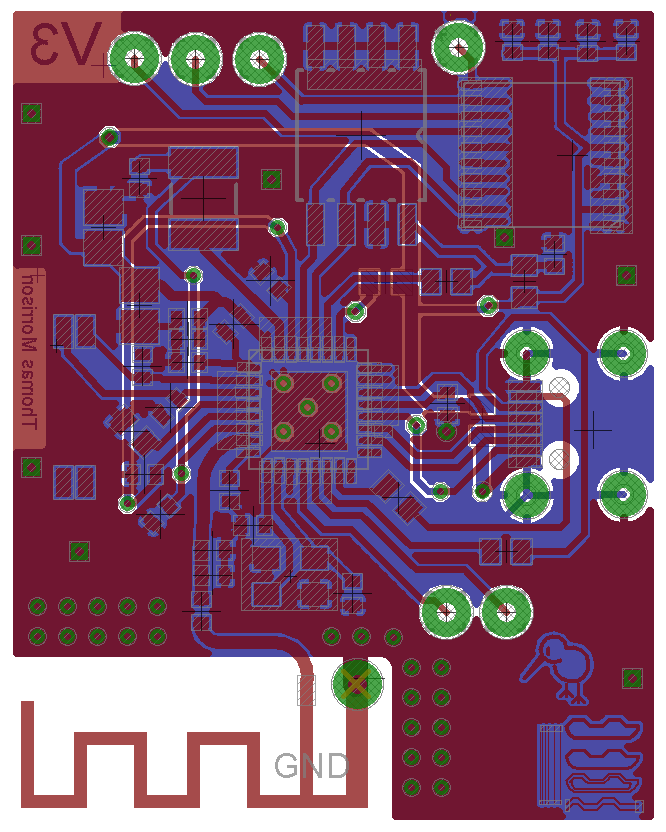
\includegraphics[width = \textwidth]{boardv1}
	\end{center}
	\caption{First (working) PCB design. Notice removal of solder mask around active components}
	\label{fig:boardv1}
\end{figure}

\begin{figure}[H]
	\begin{center}
		\includegraphics[width = 1.6\textwidth, angle = 90]{Schematic}
	\end{center}
	\caption{Schematic (showing only one ADC here)}
	\label{fig:schematic}
\end{figure}

The board was assembled by hand, and reflowed in an oven

\begin{figure}[htb]
	\begin{center}
		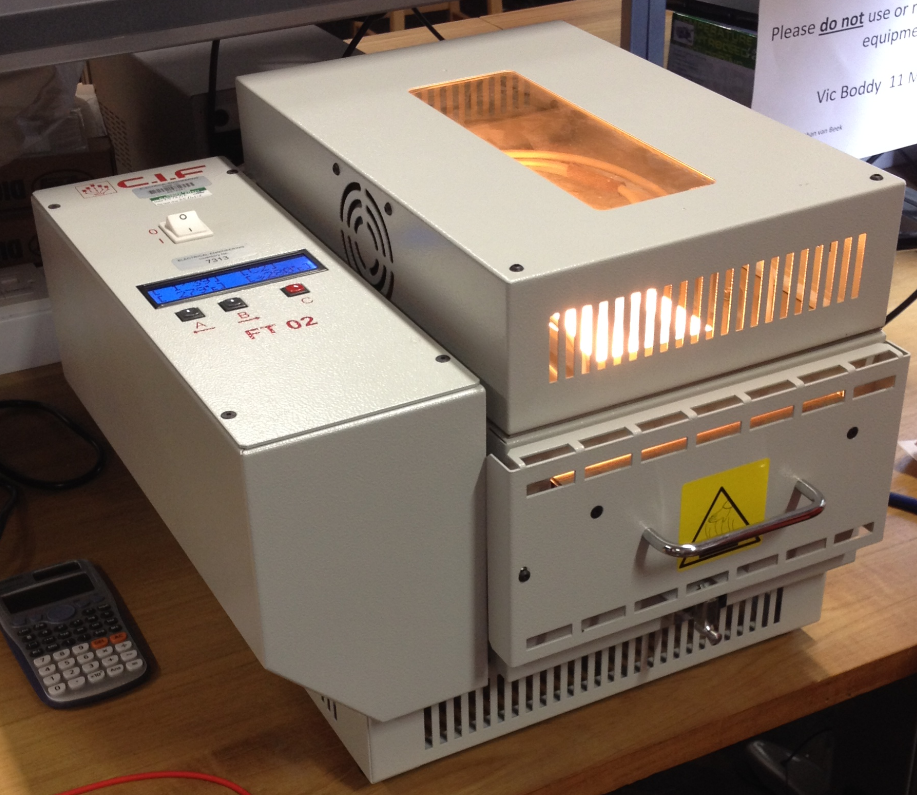
\includegraphics[width = 0.9\textwidth]{oven}
	\end{center}
	\caption{Reflow oven}
	\label{fig:oven}
\end{figure} 

During \ac{PCB} fabrication, the required feature size was below the reported capabilities of the department. Boards manufactured within the department contained a test area for discovering process capability and variation.  but through layout . The size and complexity of some of the components meant the re-flow oven did not give perfect results, and further layout techniques to assist in fabrication and assembly included removing solder resist around the active component packages, which allowed access for a soldering iron to ''touch up'' when the oven re-flow failed to perform. 

\begin{figure}[h]
	\begin{center}
		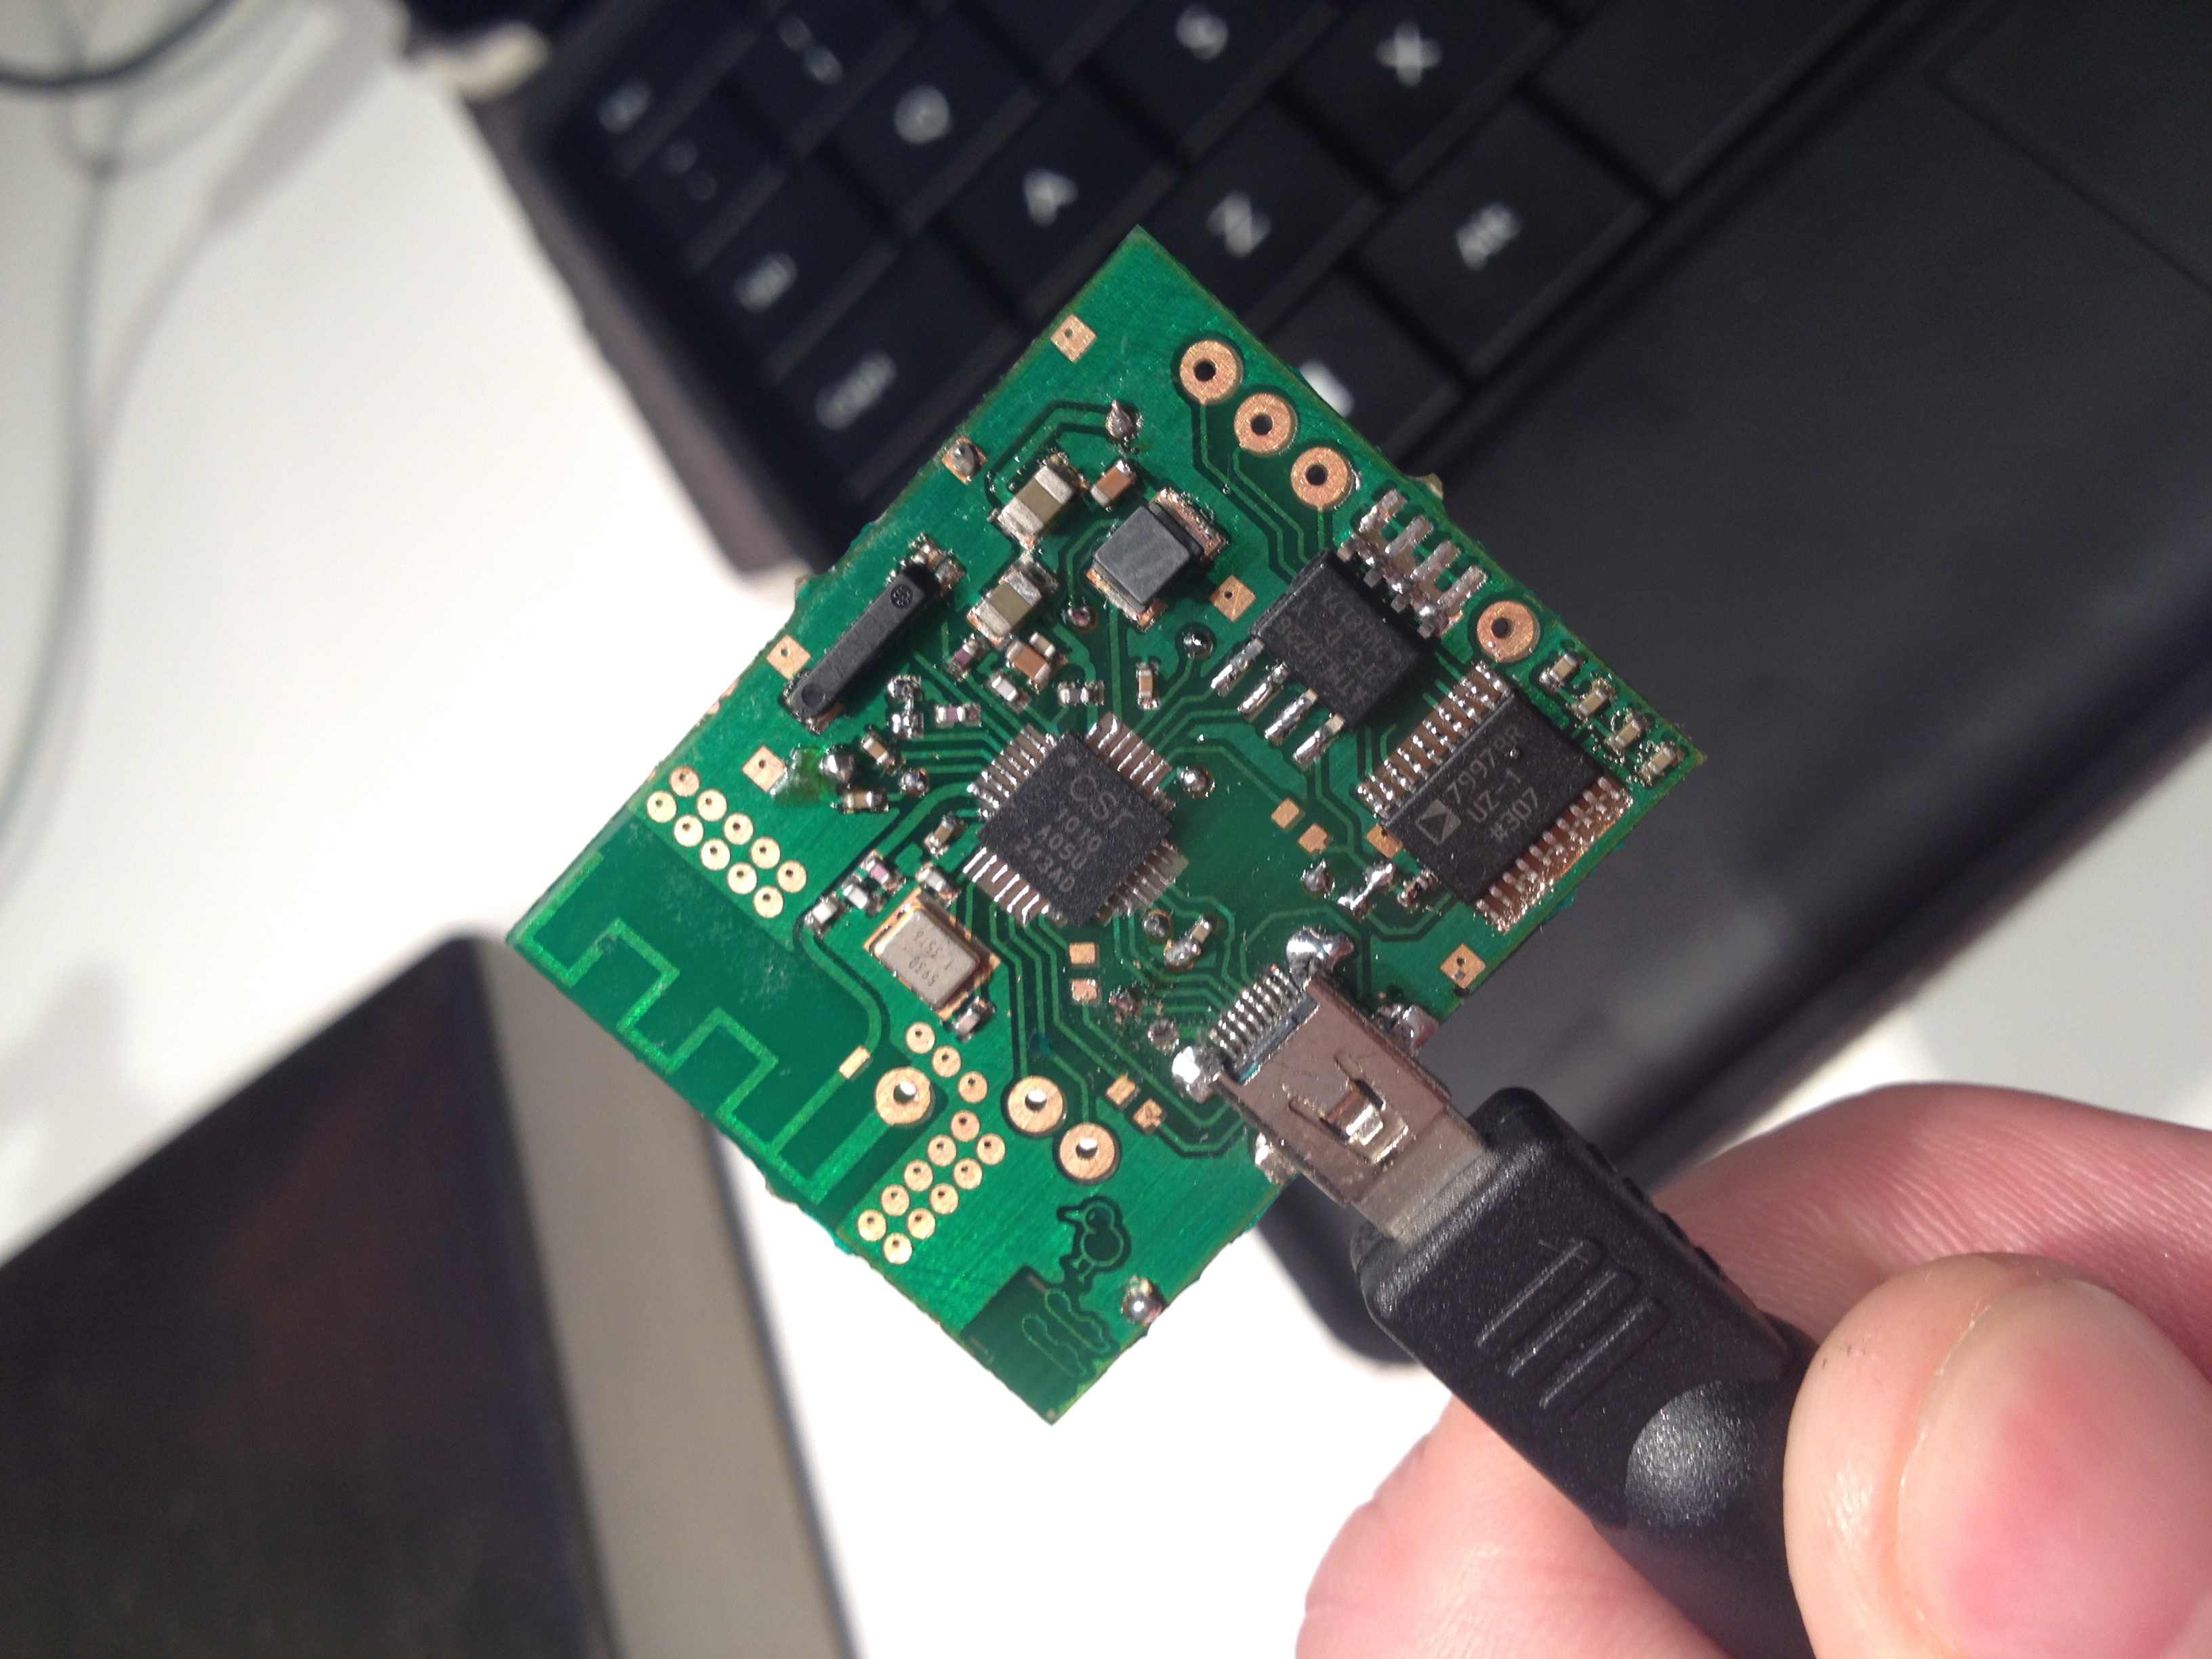
\includegraphics[width = 0.9\textwidth]{pcb1.jpg}
	\end{center}
	\caption{First (working) PCB iteration. Main components labeled. Manufactured using Imperial College London's EEE departmental facilities}
	\label{fig:pcb1.jpg}
\end{figure}

Due to the process capabilities and materials used, the radio frequency traces were not impedance matched, and the device range was limited to approximately 10 meters \ac{LOS}. 

The connector used was difficult to source, being a variant of micro-USB, yet with more pins. The pin spacing was beyond the departments capabilities, but under magnification and with the right technique it was possible to make the connections. Unfortunately, with the \ac{CAD} package did not have capabilities to draw slots required for correctly seating the 8-pin connector. The connector had to be modified and filed down to correctly sit on the board. Even with super glue, small amounts of flexing from the cable, can create enough leverage to rip the connector off the board along with the tracks, destroying direct connectivity. Two boards were damaged due to this and caused serve delays in developing the firmware for the AD7997 \ac{ADC}. A workaround, although cumbersome, was to use a smaller, breakout board to connector to the main board to prevent any damage to the main board. 

\begin{figure}[htb]
	\begin{center}
		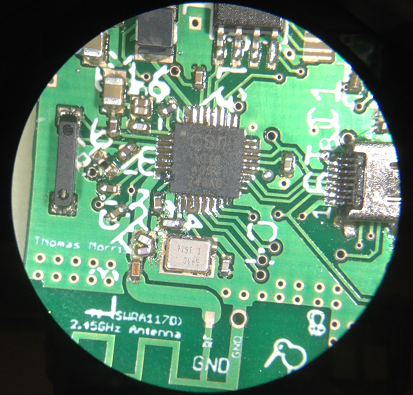
\includegraphics[width = 0.9\textwidth]{center}
	\end{center}
	\caption{\ac{QFN} touch up with a iron. Solder resist purposefully removed around small active packages, and straight tracks used to encourage solder capillary action}
	\label{fig:center}
\end{figure} 

\begin{figure}[htb]
	\begin{center}
		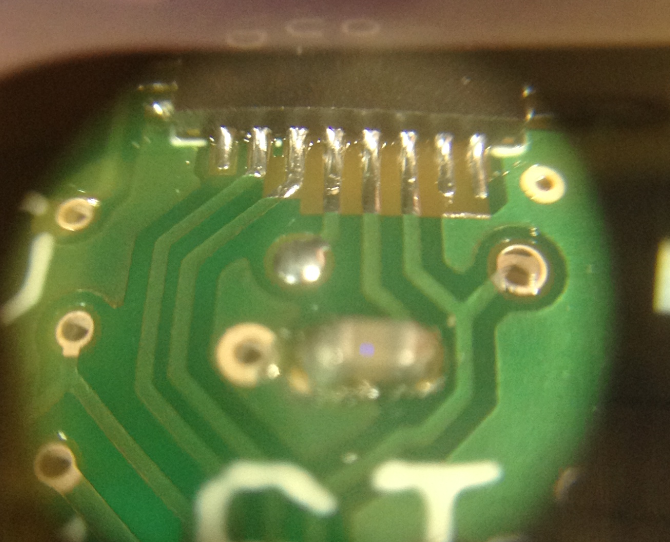
\includegraphics[width = 0.9\textwidth]{side}
	\end{center}
	\caption{High magnification, shallow depth of field. Pads on side of \ac{QFN} useful to ensure connection}
	\label{fig:side}
\end{figure} 

The second design added connections for Zinc-air battery holders, another \ac{ADC}, channel and debug pads/test points, reduced weight and theoretically better RF properties. Further, the final design was produced in a professional off-site \ac{PCB} house, making use of \ac{PTH} technology.

\begin{figure}[htb]
	\begin{center}
		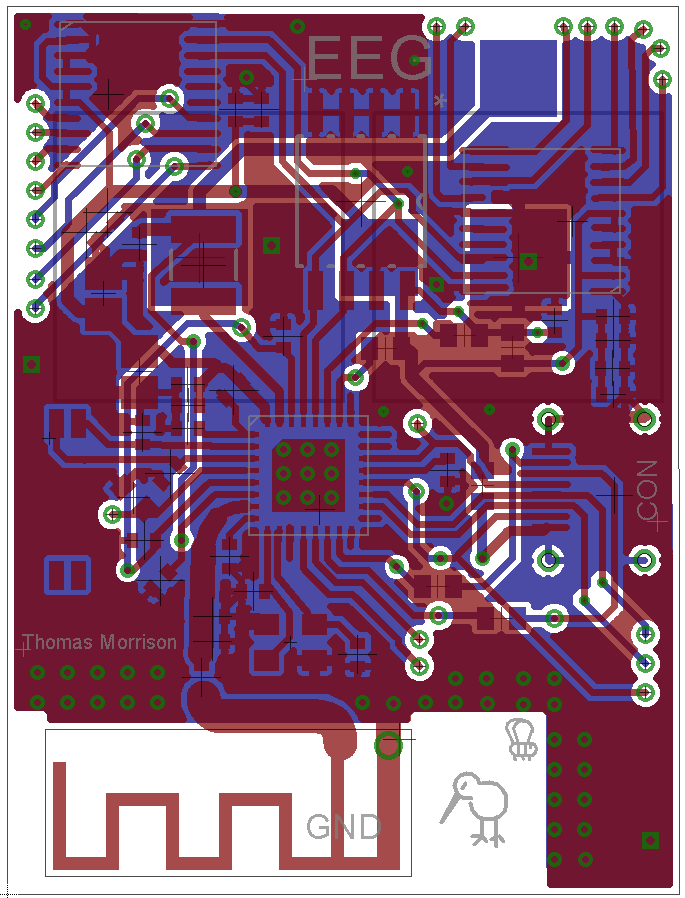
\includegraphics[width = 0.9\textwidth]{boardfinal}
	\end{center}
	\caption{Final PCB design}
	\label{fig:boardfinal}
\end{figure}

This board, while small, can be shrunk further in size through layout and manufacturing capabilities. This was not done due to increasing difficulty of assembly, time taken for optimising the layout and limitations of the departmental equipment available. 


\clearpage
\subsection{Firmware}

The CSR1010 micro-controller contains a custom processor known as the XAP, a 16 bit \ac{RISC} processor. \ac{CSR} provides the necessary tools to translate high level structured C-code into byte code instructions for the XAP processor

Fortunately, \ac{CSR} provided example projects which contains the majority of the application layer functionality (see \ref{fig:blearch}) to handle basic device operations and radio. The \ac{MCU} is a single threaded processor, yet the application design is event driven using a large central message pump(s) to service events and provide the control flow. Events can be of software origin (i.e. a flag set) or hardware invoked (hardware interrupts). Further, hardware interrupts (such as PIO) can be supported outside the software message pump. Being event driven means the use of callbacks are used frequently throughout the code base. \ac{CSR} exposes \ac{API}s to communicate with the time critical and complex host and controller layers beneath.


\begin{figure}[htb]
	\begin{center}
		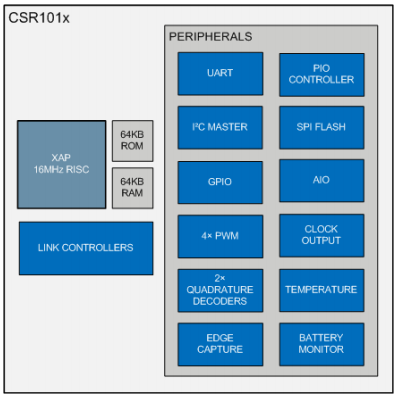
\includegraphics{mcu}
	\end{center}
	\caption{MCU overview \cite{firmwaredev}}
	\label{fig:mcu}
\end{figure}

When the device first powers up it enters the application layer through the AppInit procedure. This procedure initialises hardware and high level stack components such as the GATT server database. Once complete the control flow enters the system event message pump (AppProcessSystemEvent), which is called by the firmware to handle system level events such as PIO level changes such as configured interrupt from pins or wake events. This also handles low battery events. AppProcessLMEvent handles link manager related events from firmware. Such events include radio events (such as the acknowledgment or receipt of data) along with security manager and GAP and G(ATT) messages. Making an insertion into this latter message pump was crucial for enabling the device to transmit more notifications once data was acknowledge (indicating the buffers were free). The link manager event caught is known as LS\_RADIO\_EVENT\_IND, where the IND is short for indication - despite the packet types used being notification, this event structure also corresponds to notifications. Finally, the timers run on top of the hardware with microsecond accuracy and can be used as interrupts. They are used to wake the device out of sleep ready for communicating or doing other work. A timer structure contains a pointer to a event handler which is fired upon timer exhaustion. Once the event handler returns, the chip will power down to a dormant state until the next \ac{CE} or timer is available. It is highlighted that the application timers are not used for radio timings (i.e. synchronisation between devices happens in the base levels of the stack and/or use of dedicated hardware timers).


\begin{figure}[htb]
	\begin{center}
		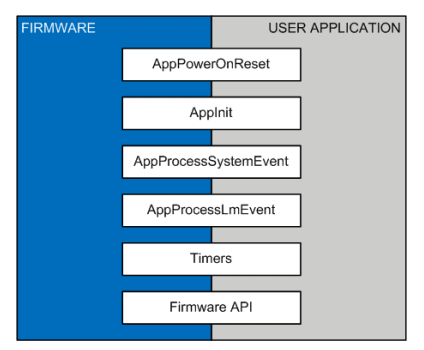
\includegraphics{flow}
	\end{center}
	\caption{Firmware - Overview of the application layer control flow \cite{firmwaredev}}
	\label{fig:flow}
\end{figure}


\begin{figure}[htb]
	\begin{center}
		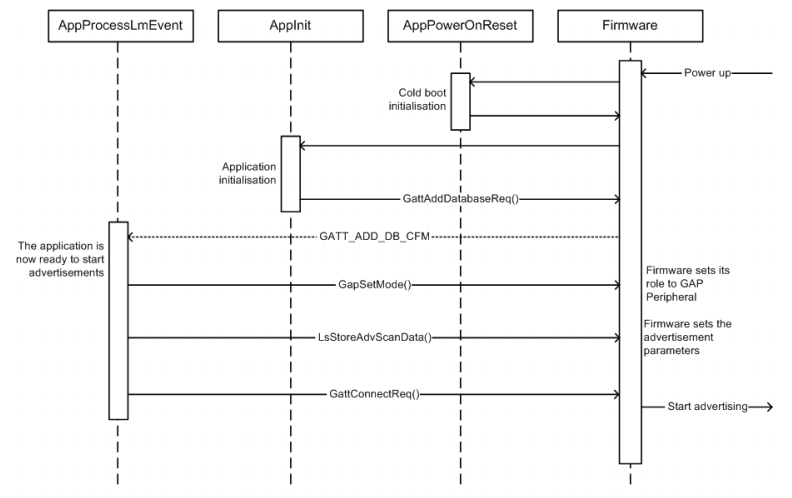
\includegraphics[width = 0.9\textwidth]{uml}
	\end{center}
	\caption{UML sequence diagram detailing power on to advertising packet events \cite{firmwaredev}}
	\label{fig:umlseq}
\end{figure}


The \ac{GATT} services and characteristics are stored in a flat-file database and defined as structures in JSON. The EEG characteristic is shown below in Listing~{lst:eeggatt}. The EEG measurement characteristic provides a notification property which allows a device to subscribe to notification messages when generated from the device.

\begin{lstlisting}[language=C, caption=GATT database entry for EEG characteristic,label={lst:eeggatt}]
#ifndef __EEG_SERVICE_DB__
#define __EEG_SERVICE_DB__

#include "eeg_service_uuids.h"

primary_service {
    uuid : UUID_EEG_SERVICE,
    name : "EEG_SERVICE",

    /* Characteristics support IRQ flag, thereby reads 
     * and writes on characteristic configuration descriptor and notifications 
     * on characteristic value are handled by application. 
     */

    /* Notifications for the data*/
    characteristic {
        uuid : UUID_EEG_MEASUREMENT,
        name : "EEG_MEASUREMENT",
        properties : notify,
        flags : FLAG_IRQ,

        client_config {
            flags : FLAG_IRQ,
            name : "EEG_MEASUREMENT_C_CFG"
        }
    },

    /* Acquisition rate (i.e. frequency)*/

    characteristic {
        uuid : UUID_EEG_ACQUISITION_RATE,
        name : "EEG_ACQUISITION_RATE",
        properties : [read, write],
        flags : FLAG_IRQ,
        value : DEFAULT_ACQUISITION_RATE
    },

    /* Number of channels*/

    characteristic {
        uuid : UUID_EEG_CHANNELS,
        name : "EEG_CHANNELS",
        properties : [write, read],
        flags : FLAG_IRQ,
        value : 0x00
    }
},
#endif /* __EEG_SERVICE_DB__ */
\end{lstlisting}

Each service and characteristic requires a \ac{UUID}, which is a string of 128 bits and due to the enormous space are very unlikely to appear elsewhere. Only 16 bits (known as the short \ac{UUID}) are required to be set as the remaining bits are previously tied to the device address, which includes specific bit patterns allocated to chip manufacturers. Further some \ac{UUID}s are reserved for predefined services and characteristics (see \url{http://developer.bluetooth.org/gatt/services/Pages/ServicesHome.aspx}). The characteristic \ac{EEG} service has the short \ac{UUID} 0xEE0 (hexadecimal), while the characteristics share a similar short-UUID. The full service UUID can be seen in the User Guide section. 

When the program is compiled the GATT data flat file is translated into a managed binary data structure and the tool chain creates events that can be referenced in the C-program. For example, EEG\_ACQUISITION\_RATE is associated with the event handle HANDLE\_EEG\_ACQUISITION\_RATE, which is contained with the EEG service message pump AcqusitionHandleAccessWrite. AcqusitionHandleAccessWrite is in turn part of the more generic HandleAccessWrite that sits within the EEG service. Interestingly, this type of pattern is well suited to object oriented paradigm, however, the compiler (as with most embedded systems) was not C++ capable. 

A shared data structure is used for each service provided. \ref{lst:eegstruct} shows the structure for the \ac{EEG} service. 

\begin{lstlisting}[language=C, caption=\ac{EEG} data structure,label={lst:eegstruct}]
typedef struct
{
    /* Energy Expended Value */

    /* Heart rate measurement client configuration */
    gatt_client_config             eeg_meas_client_config; 

    /* Offset at which Battery data is stored in NVM */
    uint16                         nvm_offset;
    
    uint16                         channel_map; 
    
    uint16                         acquisition_rate;
    
    timer_id                       acq_tmr;
    
    uint8                          measurement_buffer_1[32];
   
    uint8                          measurement_buffer_2[32];
    
    uint8                          current_buffer;

} EEG_SERV_DATA_T;
\end{lstlisting}



\begin{lstlisting}[language=C, caption=UUIDs EEG service,label={lst:eeguuid}]
#ifndef __EEG_SERVICE_UUID_H__
#define __EEG_SERVICE_UUID_H__

/*============================================================================*
 *  Public Definitions
 *============================================================================*/

/* UUIDs for EEG service and Characteristics*/

#define UUID_EEG_SERVICE			0x0EE0

#define UUID_EEG_MEASUREMENT		0x0EE1

#define UUID_EEG_ACQUISITION_RATE	0x0EE2

#define UUID_EEG_CHANNELS			0x0EE3

#define DEFAULT_ACQUISITION_RATE		0xFF



#endif /* __EEG_SERVICE_UUID_H__ */
\end{lstlisting}


\begin{figure}[H]
	\begin{center}
		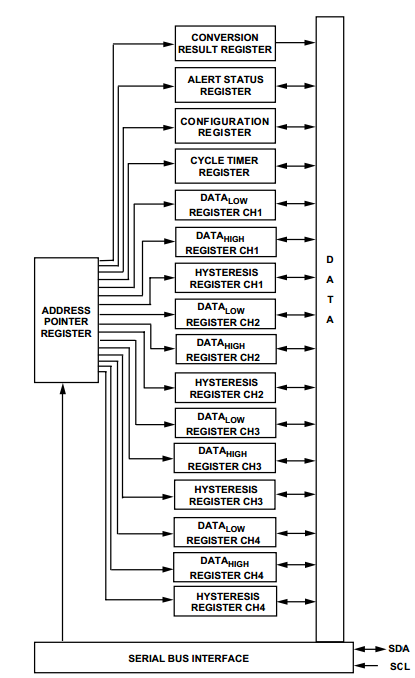
\includegraphics[width = 0.9\textwidth]{regs}
	\end{center}
	\caption{Register file}
	\label{fig:regs}
\end{figure}

To communicate with the off-chip \ac{ADC}, the I2C bus was used. The data sheet for the \ac{ADC} (AD7997) \cite{ad7997} shows the device has 3 modes of operation. Mode 1 uses edge triggering on the CONVST pin to begin a conversion. Mode 2, known as command mode allows a conversion to occur from a command sent over the I2C bus. The third and final mode is automatic cycle interval, which will cause the \ac{ADC} to power up and take measurements periodically. At the time of writing, the current implementation uses the 2nd mode, whereby the a master write to the slave causes a conversion to begin, which is read back. 

The general mechanism for communicating with the AD7997 \ac{ADC} over the I2C bus is as follows. A start command is sent out from the master CSR1010, which causes all I2C devices to listen. A 7 bit device address is sent out on the bus along with a access bit (representing read or write). Devices will shift in these 8 bits, and any devices which match the 7-bit address with acknowledge the master. This process is known as I2C serial addressing. Once the device acknowledges, the register address currently residing the address register of the \ac{ADC} can be read or written to, but not both within the operation (serial addressing must be done again to change access). The available registers can be seen in Figure~\ref{fig:regs}. For the project only the address pointer, conversion and configuration registers are of interest. 

To configure the channel map the master first writes the configuration register address (0x02) to the address pointer register, referencing the correct register from the register file, then writes two bytes of data which contain the channel map (along with some other bits \ref{fig:configreg}). Listing~\ref{lst:adc} shows the configuration of channels for the \ac{ADC} over the I2C bus, and can be visualised from \ref{fig:waveform}.


\begin{lstlisting}[language=C, caption=ADC I2C bus channel map configuration,label={lst:adc}]
    /*Serial address all devices on bus*/
    I2cRawCommand(i2c_cmd_send_start, TRUE, I2C_WAIT_ACK_TIMEOUT);
    I2cRawWriteByte((0b010001 << 2) | (CHIP_NUMBER << 1) |  CMD_WRITE);
    /*Write to address register the address of the configuration register */
    I2cRawCommand(i2c_cmd_wait_ack, TRUE, I2C_WAIT_ACK_TIMEOUT);
    I2cRawWriteByte(0b00000010);
    I2cRawCommand(i2c_cmd_wait_ack, TRUE, I2C_WAIT_ACK_TIMEOUT);  
    /*Configuration register write, D11-D4 are the channel map*/
    I2cRawWriteByte(0b00000000 | CHANNEL_MAP_HALF >> 4);
    I2cRawCommand(i2c_cmd_wait_ack, TRUE, I2C_WAIT_ACK_TIMEOUT);  
    I2cRawWriteByte(CHANNEL_MAP_HALF << 4 | 0b0000000);
    I2cRawCommand(i2c_cmd_wait_ack, TRUE, I2C_WAIT_ACK_TIMEOUT);  
    
    I2cRawCommand(i2c_cmd_send_stop, TRUE, I2C_WAIT_ACK_TIMEOUT);
\end{lstlisting}


\begin{figure}[H]
	\begin{center}
		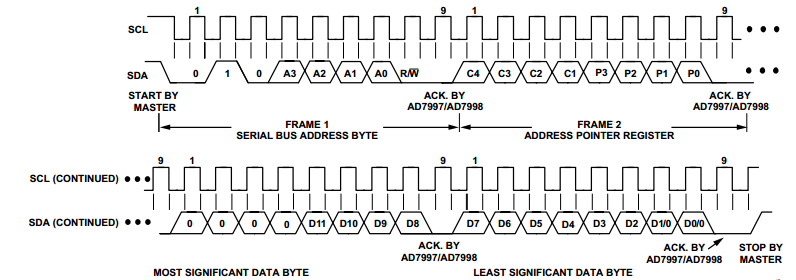
\includegraphics[width = 0.9\textwidth]{waveform}
	\end{center}
	\caption{Configuration register that controls which channels are activated}
	\label{fig:waveform}
\end{figure}

To permit more than one AD7997 \ac{ADC} on the I2C at one time, depending on the connectivity of the AS (15) pin, the 7-bit I2C address will vary. To create a bigger address space, the AD7997 \ac{ADC} comes in two variants - the "/0" and "/1", meaning upto a total of 6 chips can be directly connected to the bus. It can be seen from \ref{fig:boardfinal} that one \ac{ADC} has its AS pin floating and the other \ac{ADC} has AS tied to ground. This is represented by CHIP\_NUMBER in \ref{lst:adc}. Further, as each AD7997 \ac{ADC} sports only 8 channels, the 16bit channel mask contained with the firmware is divided between each \ac{ADC}, represented by CHANNEL\_MAP\_HALF .


\begin{figure}[H]
	\begin{center}
		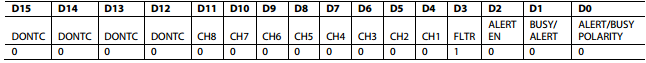
\includegraphics[width = 0.9\textwidth]{configreg}
	\end{center}
	\caption{Configuration register that controls which channels are activated}
	\label{fig:configreg}
\end{figure}


Note that the data sheet \cite{ad7997} required the device to have an external pull-up resistor, which is provided by a configurable internal pull up on the SDA and SCL lines of the CSR1010.


\begin{lstlisting}[language=C]
    I2cInit(I2C_RESERVED_PIO , I2C_RESERVED_PIO , I2C_POWER_PIO_UNDEFINED, pio_mode_strong_pull_up);
    I2cConfigClock(I2C_SCL_100KBPS_HIGH_PERIOD, I2C_SCL_100KBPS_LOW_PERIOD);
    I2cEnable(TRUE);
\end{lstlisting}













\subsection{Tablet Application}

The high level tablet application was written for Microsoft's .NET framework platform in C\#. The application relied upon the GenericAttributeNamespace (specifically $Windows.Devices.\\Bluetooth.GenericAttributeProfile$) class library to communicate with \ac{BLE} devices. The application uses the new WinRT application design introduced into the Windows operating system since Windows 8. Writing for WinRT means the application can be easily be ported between a tablet to a Windows OS phone The application architecture makes full use of \ac{OOP}, with an emphasis on the \ac{MVVM} design pattern. The application was design to allow the user to be able to connect to a device, select the number of channels measure and the frequency. 

The View is written in a markup language known as \ac{XAML}. This is a verbose, but rich markup that allows a \ac{GUI} to be highly flexible. It is what describes the view of the model (data) and binds to the view-model. The view-model, which is similar to the controller in the \ac{MVC} pattern is the code behind (C\#) which can be thought of as a "value converter", meaning it is tasked with exposing the model's data objects for easy consumption and manageability. This is subtly difference from the controller, which tells the view what to display and when. An example of the View-Model would be a collection (e.g. a list of \ac{EEG} measurements), that when mutated, automatically update the \ac{GUI}. In the context of \ac{XAML} and \ac{MVVM}, this is known as data binding, and allows the View to easily consume the model.

In the context of a \ac{BLE} service, the \ac{EEG} service is described by the data model shown in Figure~\ref{fig:classdiagram}. The model contains \ac{EEG} specific members such as the acquisition rate, channel map and the data for each channel. The model also contains some house cleaning members, such as the service and IsInitialised variables. As only one \ac{EEG} service can exist, it made sense to implement a singleton pattern to allow easy lifetime and access from the model to the view-model. While singletons are often associated with poor \ac{OOP} design, the simplicity afforded by their use here make sense for the implementation. The SwapUInt16 method is required when writing data back to the CSR1010, as the device word size 16 bit, with big endianess (x64 is little-endian). The eegChannels data member contains . However, the method eegNotification can be used to provide direct access to the incoming notifications, acting as the callback from notification events.

\begin{figure}[htb]
	\begin{center}
		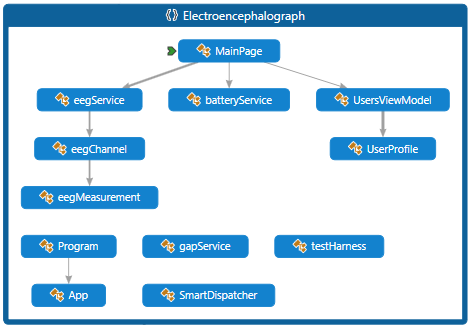
\includegraphics[width = 0.9\textwidth]{dep}
	\end{center}
	\caption{Dependencies}
	\label{fig:dep}
\end{figure}

\begin{figure}[htb]
	\begin{center}
		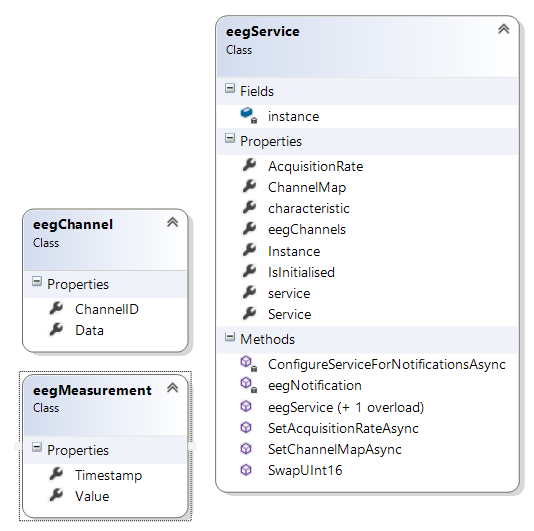
\includegraphics[width = 0.9\textwidth]{classdiagram}
	\end{center}
	\caption{Data model (class diagram) for the \ac{EEG} service}
	\label{fig:classdiagram}
\end{figure}

The GenericAttributeNamespace provided by the .NET framework provides functionality on the work at the \ac{ATT} level. The mechanism for interfacing with the \ac{BLE} devices to to enumerate all connected devices then filter on the short \ac{UUID}. Connected devices are devices connected outside of the application (i.e. through the Windows OS Bluetooth settings from control panel - Figures~\ref{fig:connecting},~\ref{fig:dvcmgr}. This will return objects for all devices with a service matching that of the short \ac{UUID}. These objects can be further queried to find characteristics belong to this service along with the properties (read, write, indicate or notify). It is then possible to read, write or assign event callbacks from these characteristics. Attempting to write to a read only characteristic will result in an access denied, which will need to be handled to prevent program termination.  

%cba to get c# print, c++ will do
\begin{lstlisting}[language=C++, caption=Connecting to a \ac{BLE} device's \ac{EEG} service ,label={lst:csharpeble}]

            var devices = await Windows.Devices.Enumeration.
		DeviceInformation.FindAllAsync(GattDeviceService.GetDeviceSelectorFromShortId(0xEEE0));

            if (devices.Count < 1)
            {
                await new MessageDialog("Could not locate any EEG devices in the vinicity").ShowAsync();
                return;
            }

            //By default connect to the first EEG service found
            eegService.Instance.service = await GattDeviceService.FromIdAsync(devices[0].Id);
	//Use long GUID with 16 bit short UUID  (could of used just shortID) 
            var eegData = eegService.Instance.service.GetCharacteristics(new Guid("0000EEE1-0000-1000-8000-00805f9b34fb"))[0];
	//Define call back function
            eegData.ValueChanged += eegData_ValueChanged;

\end{lstlisting}

The applications makes extensive use of the \ac{TPL} for a fluid and responsive \ac{GUI}. The \ac{TPL} uses asynchronous procedures to add parallelism and concurrency. This is particularly useful in this application, as the \ac{GUI} thread needs to be constantly updated from incoming data without preventing usability. Despite use of the \ac{TPL} further timing mechanisms were required to prevent interface lock up. When new data comes from the device, it will be transposed into the model. This will cause the data binding between the view and model to signal a change, meaning the view updates. Due to the high throughput, this mechanism can cause great delay, and hence, batching the updates is preferred (listing~\ref{lst:csharpeble}).

%cba to get c# print, c++ will do
\begin{lstlisting}[language=C++, caption=Batch update code (for generic types),label={lst:csharpeble}]

	//For a single graph (can be called for each graph)
        private void batchUpdate(ThreadPoolTimer source)
        {
            
                AddItem<FinancialStuff>(financialStuffList, lst);                        

        }

	//Pass an obversable collection (databound object between the model and the view), and a list of items to append to the collection
        public async void AddItem<T>(ObservableCollection<T> oc, List<T> items)
        {

                //data points to keep on the graph
                const int maxSize = 500;

                // Make sure it doesn't index out of bounds
                int startIndex = Math.Max(0, items.Count - maxSize);
                int length = items.Count - startIndex;

                List<T> itemsToRender = items.GetRange(startIndex, length);

                lst.Clear();

                 await  Task.Factory.StartNew(() =>                
                {
                    lock (oc)
                    {
                        oc.Clear();

                        for (int i = 0; i < itemsToRender.Count; i++)
                        {
                            oc.Add(itemsToRender[i]);
                        }
                    }
                });
        }

...

	//Establish the timer object with a handler -  100 milli second update
            periodicTimer = ThreadPoolTimer.CreatePeriodicTimer(new TimerElapsedHandler(batchUpdate);, new TimeSpan(0, 0, 0, 0, 100000));
\end{lstlisting}


\begin{figure}[htb]
	\begin{center}
		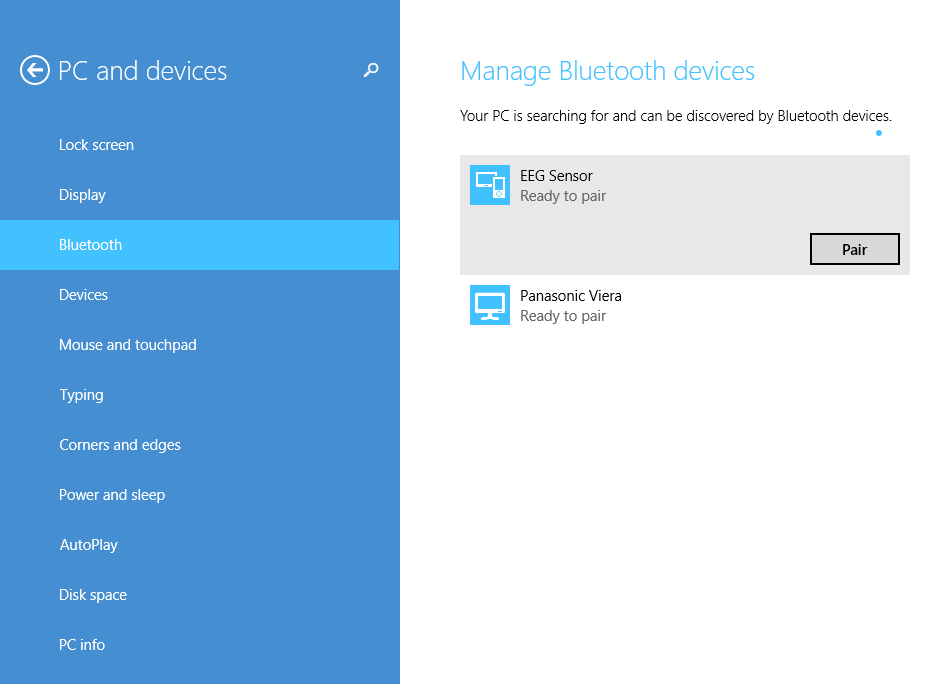
\includegraphics[width = 0.9\textwidth]{searching}
	\end{center}
	\caption{Searching for Bluetooth devices in windows}
	\label{fig:searching}
\end{figure}

\begin{figure}[htb]
	\begin{center}
		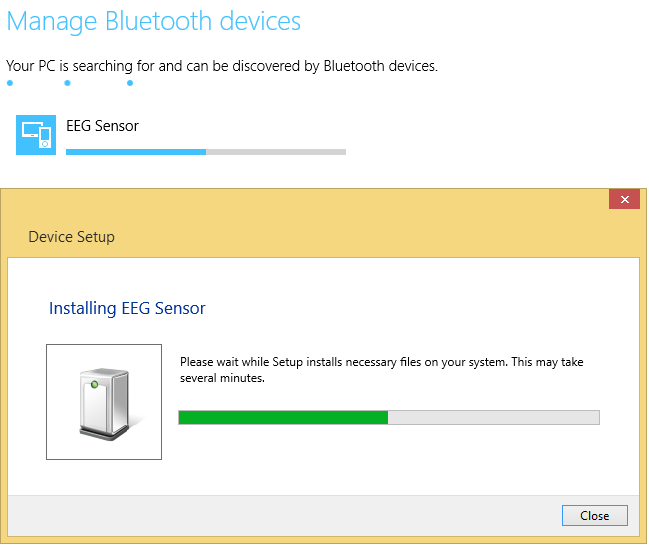
\includegraphics[width = 0.9\textwidth]{connecting}
	\end{center}
	\caption{Connecting and installing to a \ac{BLE} device}
	\label{fig:connecting}
\end{figure}

\begin{figure}[htb]
	\begin{center}
		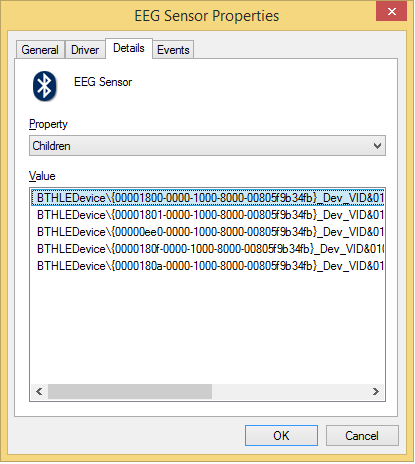
\includegraphics[width = 0.9\textwidth]{dvcmgr}
	\end{center}
	\caption{\ac{EEG} sensor installed as a Bluetooth device. Long UUIDs for each service present on the device}
	\label{fig:dvcmgr}
\end{figure}


At the time of writing the application looks like


\begin{figure}[htb]
	\begin{center}
		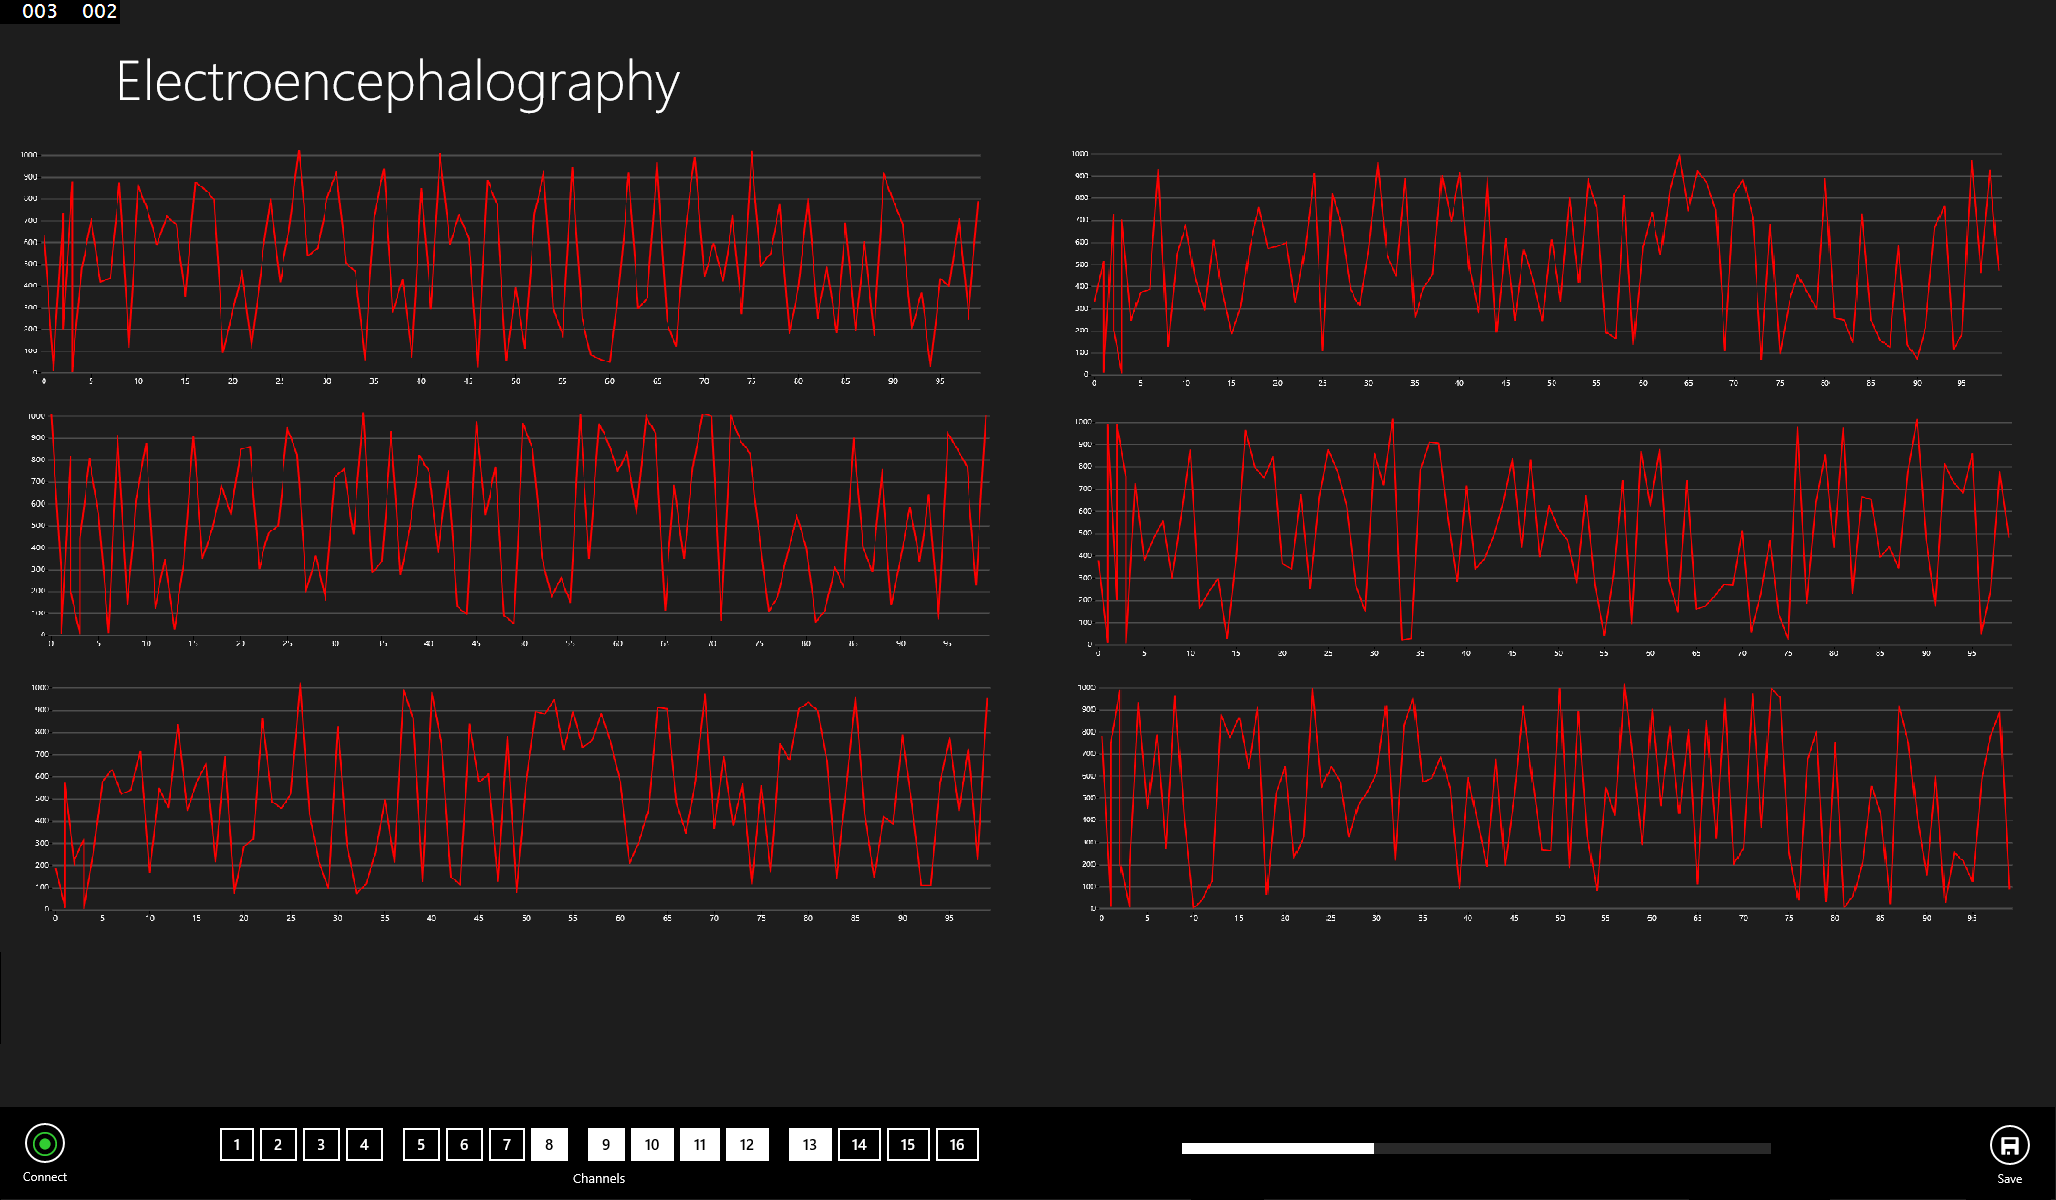
\includegraphics[width = 1.4\textwidth,angle = 90]{exampleapp}
	\end{center}
	\caption{Application - 6 channels configured, with real time update}
	\label{fig:exampleapp}
\end{figure}






An issue was found whereby at higher throughputs, the order in which notifications are received become handled out of order. The reason for this occurring is that there is no guarantee when events are dealt with. Every time a packet is received, it will fire an event handler, however this will occur in batches. If the rate at which these batches is processed is greater than the rate at which new events arrive, then the events may no be handled in order. Unfortunately, there has been no fix for this, and it is assumed a current limitation of Microsoft's .NET GenericAttributeNamespace. When using the \ac{CSR} stack and \ac{SDK}, the events are handled in the order they occur. Despite this causing issues in the high level application, for the remainder of this report it is ignored. Microsoft has since been contacted about the issue and are looking into it. It is understandable that they wouldn't of built the system for it (much like how some manufacturers only permit a limited amount of packets per \ac{CE}), but even at smaller throughputs, notifications from the same service may be serviced out of order. 





\clearpage



\clearpage
\section{Evaluation}

\subsection{Throughput}
\label{sec:Throughput}

In the sole pursuit of maximizing throughput, the idea to try and pack as many notifications into a \ac{CE} is a superficial tactic. Taking the smallest \ac{CI} of 7.5ms, upto $\frac{7500}{676} = 11.094675$ packets can fit into this interval. This 0.094675 remainder may seem small, and indeed equates to only 13 packets lost of the maximum throughput within a second, thus reducing the total throughput by less than 1$\%$. This remainder changes with the \ac{CI} and in the worst case, just less than a whole packet fits into the remaining space. The profile which describes the "remainder" packets is formally written as

\begin{displaymath}
 \frac{1250\times x}{676}  - \floor{ \frac{1250\times x}{676}}
\end{displaymath}

where 1250 is the \ac{CI} unit, x the value, 676 the round-trip time for a maximum size data packet. A connection interval must be between 7.5ms and 4000ms long, in incremental steps of 1.25ms. Therefore x must exist in the range of 6 to 3200. This can be visually depicted as

\begin{figure}[H]
	\begin{center}
		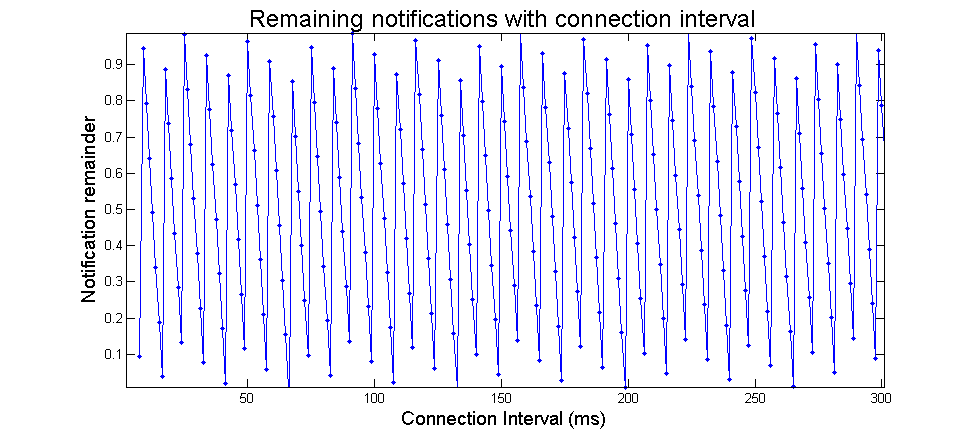
\includegraphics[width = \textwidth]{notremain}
	\end{center}
	\caption{Remainder of packets unabel to fit into \ac{CI}}
	\label{fig:notremain}
\end{figure}

However, this is simply the plot of the remainder, and for higher \ac{CI} there will be more packets per \ac{CE} and therefore while the remainder may be bigger, the throughput may be higher than a smaller \ac{CI} with a smaller remainder. That is, the throughput is the number of \ac{CE}s in a given time frame multiplied by the number of packets per \ac{CE}. Factoring this in, the description changes to

\begin{displaymath}
 \frac{1}{1250 \mu s \times x} \times \floor{ \frac{1250 \mu s\times x}{676 \mu s}} \times 160 bits 
\end{displaymath}

This produces an expression for the maximum throughput against \ac{CI}, shown graphically below


\begin{figure}[H]
	\begin{center}
		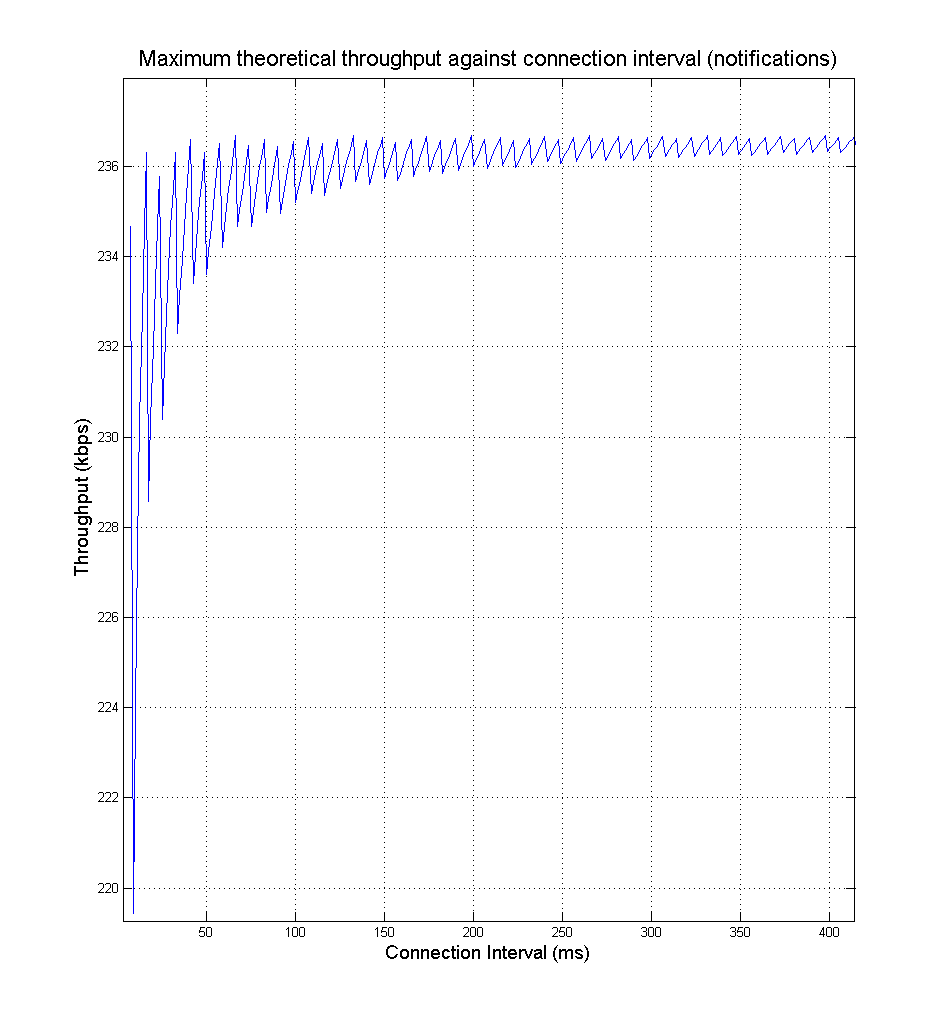
\includegraphics[width = \textwidth]{throughput}
	\end{center}
	\caption{Throughput varying with connection interval}
	\label{fig:throughput}
\end{figure}

The throughput tends asymptotically to the maximum of 236.686 kbps, and min to max throughput is above 7$\%$. To investigate how the theoretical maximum profile compares to the actual in practice, a test harness was created to investigate the relationship between throughput and \ac{CI}. The test harness writes to the \ac{GAP} characteristics the desired \ac{CI} then takes a measurement of average throughput over a few minutes. It then moves onto another \ac{CI} and does the same thing. This is called a test set. Sets are repeated a desired number of times (at least 3) and averaged as it was found that there is a variation between sets. The results produced the profile shown in Figure~\ref{fig:civsdatarate}.



\begin{figure}[H]
	\begin{center}
		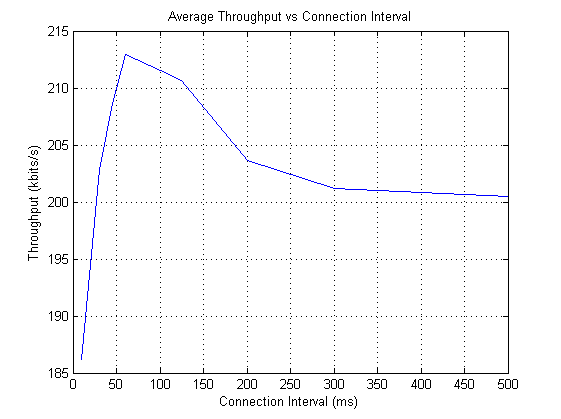
\includegraphics[width = \textwidth]{civsdatarate}
	\end{center}
	\caption{How throughput changes with varying connection interval}
	\label{fig:civsdatarate}
\end{figure}

It was found that the optimum throughput did not exist at the longest connection interval. Rather, the profile appears have a single peaked platykurtic shape. The specification requires that during a \ac{CE}, transmission errors (e.g. a CRC error), should cause the devices to "give up", power down and wait until the next interval to begin communicating again. This means that while longer \ac{CI}s have marginally more throughput,  there exists a trade off between the \ac{CI} and risk of premature link termination. Figures~\ref{fig:2sec}, ~\ref{fig:lowcierrors} shows packet waveforms for short and long \ac{CI}. These were captured through use of a shunt resistor (see \ref{Power Analysis}). It can be seen that the longer \ac{CI} intervals are prematurely terminated much more frequently than the shorter \ac{CI}s. It is proposed that this exists because all communications takes place on the same channel during a single \ac{CE}. In the subsequent \ac{CE} the channel channel. For longer \ac{CI}s, the chance of interference on that channel increases, while this is vice versa for shorter \ac{CI}s. An more analytic approach is shown in a 2011 IEEE communications letter \cite{Gomez2011}, however does not take into account the remainder problem, showing it's possible to achieve 236.7kbit/s with a 7.5ms \ac{CI}. It does show, however, that under a high \ac{BER}, a lower connection interval is the best strategy (Figure~\ref{fig:ber}).

\begin{figure}[H]
	\begin{center}
		\includegraphics[width = \textwidth]{ber}
	\end{center}
	\caption{Throughput against \ac{CI} for various bit error rates \cite{Gomez2011}}
	\label{fig:ber}
\end{figure}

Radio interference can described as a Poisson process, whereby radio interference is an event occurring randomly in time. This shape will change depending on the conditions of the environment the radio is used in. Therefore, the task of achieving the highest throughput collapses to being able to discover this profile. In practice this can be achieved by sampling throughput against \ac{CI} using a feedback system to find the local maximum. Investigating the range of variation between different radio environments may be an interesting piece of further work. 

\begin{figure}[H]
	\begin{center}
		\includegraphics[width = \textwidth]{2sec}
	\end{center}
	\caption{Waveform of notification packets for a \ac{CI} of 2 seconds. Majority of \ac{CE}s exhibit premature termination}
	\label{fig:2sec}
\end{figure}


\begin{figure}[H]
	\begin{center}
		\includegraphics[width = \textwidth]{lowcierrors}
	\end{center}
	\caption{\ac{CE}s with low \ac{CI}s exhibit premature termination far less than those with higher \ac{CI}s. Further, when premature termination occurs, it lasts for a shorter period as the next \ac{CE} is on average, closer in time}
	\label{fig:lowcierrors}
\end{figure}



It is believed that the maximum throughput was not reached due to transmission errors causing premature termination and device limitations. At a \ac{CI} of 60ms, transmission errors still occur as shown in Figure~\ref{fig:60ci}. Device limitations includes the apparent 1.6ms of time between each connection. This 1.6ms represents 2 full notifications packets, and can be explained as to why at 7.5ms, only a throughput of 9 packets is achieved, not 11, like the theoretical maximum predicts. No requirement of this time has been found within the specification, and it is assumed that this is a limitation of the CSR1010 device. Figure~\ref{fig:cilimit} shows this. 

\begin{figure}[H]
	\begin{center}
		\includegraphics[width = \textwidth]{60ci}
	\end{center}
	\caption{Transmission errors causing premature disconnection at 60ms}
	\label{fig:60ci}
\end{figure}

\begin{figure}[H]
	\begin{center}
		\includegraphics[width = \textwidth]{cilimit}
	\end{center}
	\caption{Radio power down present at every connection interval}
	\label{fig:cilimit}
\end{figure}

Premature termination was observed to be frequent even at relatively low \ac{CI}s. For example, at 60ms approximately 55$\%$ of 1 second samples achieved the full recorded throughput   (e.g. Figure~\ref{fig:60cithroughput}). This differs greatly to a \ac{CI} of 7.5, whereby this figure was measured close to 100\%. 

\begin{figure}[H]
	\begin{center}
		\includegraphics[width = \textwidth]{60cithroughput}
	\end{center}
	\caption{Radio power down present at every connection interval}
	\label{fig:60cithroughput}
\end{figure}




The \ac{CI} also determines the latency from when a measurement is taken to when it is displayed to the user. If data is buffered over many \ac{CE}s and/or the frequency is low, the latency can become very large. In contrast, at high frequencies, the 64 k/bytes of ram (much used for the firmware application itself), may overflow and hence buffering is not a suitable. Further, with premature \ac{CE} termination at higher \ac{CI}s, data may have to remain buffered for long as early termination prevents communication until the subsequent \ac{CE}. Providing the data can be serviced so that the buffer depth remains roughly the same over time (and does not variate to above full capacity), than selecting \ac{CI}s that cause higher premature termination but higher average throughput is a rational choice in the pursuit of high data rates, but may suffer from higher power consumption.  



The difference between the minimum and maximum throughput for the theoretical maximum vs \ac{CI} curve is approximately 7$\%$, while that derived empirically was closer to $\%$. At the peak measured performance, the device was capable of an average data rate of 90\% (213kbit/s) of the theoretical maximum (236.686kbit/s. This figure was achieved at a \ac{CI} of 60ms. In the context of an \ac{EEG} device, at this data rate the following specifications are achievable.



\begin{table}[H]
\centering
\caption{Example achievable specifications from throughput}
\label{fig:sensors}
\begin{tabular}{|p{1.1in}|p{1.1in}|p{1.1in}|p{1.1in}|} \hline 
\textbf{Channels} & \textbf{Resolution (bits)} & \textbf{Frequency (Hz)} & \textbf{Required datarate (kbit/s)} \\ \hline 
16 & 8 & 1500 & 192 \\ \hline  
16 & 8 & 1600 & 205 \\ \hline
16 & 10 & 1300 & 208 \\ \hline  
2 & 10 & 10000 & 200  \\ \hline  
16 & 8 & 1000 & 128 \\ \hline  
16 & 10 & 200 & 32 \\ \hline  
16 & 8 & 1300 & 25.6 \\ \hline  
16 & 8 & 1300 & 25.6 \\ \hline  

\end{tabular}
\end{table}




 Many devices restrict how many packets per \ac{CE} can be received, constraining the system further, and in such cases, having a smaller \ac{CI} is of benefit. The iPhone was observed to allow, on average only 6 packets per \ac{CE} and limit the \ac{CI} to a minimum of 30ms. From the Apple developer guidelines, it is possible to reduce this interval to 20ms. Many Android devices have also have restrictions on the number of packets processed. At 6 packets per \ac{CE}, and 7.5ms \ac{CI}, the throughput achievable is 128 kbit/s, which is theoretically just enough bandwidth to support 16 channels with an 8 bit resolution at 1000 Hz.

Ultimately, to maximize throughput it is important to choose a \ac{CI} for the trade off between \ac{CE} notification packing wastage, risk of premature \ac{CE} termination, latency and data integrity. The choice will further be constrained if \ac{BLE} devices are limited by the number of packets per \ac{CE}. It is believed this limitation arises from the firmware of the device as permits simpler firmware and manufacturers do not consider the use case of maximising throughput significant as there are other technologies out there. From the work above,the CSR1010 was found capable of achieving over 91\% of the theoretical maximum. While not considered relevant in the report, when devices operate at full duplex communication, the total throughput as a sum of useful (20byte notifications) in each direction is approximately 358.8kbps. This means both the peripheral and master send 296 bit notification packets, in which the header acknowledges the other. All measurements were taken within a 1 meter range between the dongle and receiver, however background radio noise was outside of the project's control.













\clearpage
\subsection{Power Analysis}
\label{sec:Power Analysis}
To measure the power usage of the system a 10 ohm shunt resistor was inserted between the board's $V_{ss}$ and ground. Scope leads where then attached to measure the voltage, which due to ohm's law, will be measured at 10 times the current. 

Firstly, the power usage of the just the radio was performed (the ADCs were disconnected).  The data sheet claims the maximum peak current used during transmission or receiving is approximately 16mA at 3V. While the measurements in Figure~\ref{fig:ceclose} and Figure~\ref{fig:ce} are at 3.3 volts, the overall power consumption of the system is the system regardless of the voltage level used. If voltage is decreased, the current increases.

\begin{figure}[htb]
	\begin{center}
		\includegraphics[width = \textwidth]{adv}
	\end{center}
	\caption{Advertising Event}
	\label{fig:adv}
\end{figure}

It can be seen from Figure~\ref{adv} that the measured voltage is 150mV. This corresponds to 15mA, approximately what the data sheet claimed. This represents an instantaneous power of 45mW. As mentioned previously, the advertising state of the system happens so infrequently that the long run cost is considered zero, hence the power analysis presented here does not include information from the advertising state (although \cite{Liu2012} seems to provide a good starting point). Interestingly, the highest peak current is measured when the device is advertising, presumably as the device is broadcasting on 3 channels, rather than just one, as once a connection has been established. 

\ac{CE}s where no data other than correspondence packets to keep the link alive, measured a peak current consumption less than 12mA at 3V. The \ac{CE} can be divided into sections - the device wakes up approximately 2 milliseconds before transmission, remains idle, then listens/transmits (receipt of information before transmission occurs first for the slave device). 

\begin{figure}[H]
	\begin{center}
		\includegraphics[width = 0.9\textwidth]{ceclose}
	\end{center}
	\caption{Connection event (3.3 volt supply)}
	\label{fig:ceclose}
\end{figure}


\begin{figure}[H]
	\begin{center}
		\includegraphics[width = 0.9\textwidth]{ce}
	\end{center}
	\caption{Connection events - connection interval set at 1 second with a slave latency of 0 (3.3 volt supply)}
	\label{fig:ce}
\end{figure}

To investigate further the power consumption, the data was logged and using an oscilloscope, saved to disk for later analysis. It was noticed that when the chip went into a deep sleep (in between \ac{CE}s), the minimum value the scope recorded was negative. To adjust for this the absolute of the minimum value was added to the whole current vector. This will bring the minimum consumption to 0, however this is still not correct as the device will consume a small amount of power in deep sleep. To correct for this, the data sheet value of 5$\mu$A was taken and applied to the current vector. 

To calculate the power consumption the trapezium rule is used to find the area under the profile. For 2.8V the area found under the curve equals. This area represents the current consumption in milli-amp-hours for a single \ac{CE} with spacing either side to tessellate with the next \ac{CE}. For each \ac{CE}, a total of 2.69mA is consumed.  To convert this to the current consumption in units milli-amp-hour not per connection event, the number is multiplied by the number of connection events (set by the connection interval) within an hour period, and divided through by the number of milliseconds in an hour to convert the time units (the x-axis in Figure~\ref{fig:icur2.8} is in milliseconds). 

Below shows the corrections and simple current consumption correction script for MATLAB. 

\begin{lstlisting}
current = Volt / 10; %adjust voltage to current (divide by 10 as 10 ohm shunt resistor)
currentAdjusted = current + abs(min(current)) + 0.000005 %voltage/current should not be negative. Shift up by absolute most negative value and add 5 micro amps taken from data sheet
\end{lstlisting}

However this often produces idle periods greater than 5 $\mu$A, so an alternative method can be used:

\begin{lstlisting}
currentAdjusted = current - mean(current(1:300)) + 0.000005 %first 300 samples should be while device is sleeping. This should average to 5 micro amps
\end{lstlisting}

This is more accurate in producing profiles where at sleep time, the current is very close 5 $\mu$As.

\begin{figure}[H]
	\begin{center}
		\includegraphics[width = 0.9\textwidth]{icur28}
	\end{center}
	\caption{Connection event (3.3 volt supply)}
	\label{fig:icur2.8}
\end{figure}

%This 2.69mA or (7.532mW power for all voltages) is the "base" amount, which must be at least consumed every time data the slave communicates.
 The rush current and idle time represents a fixed cost associated with communicating with the master, and to achieve a higher economical value of energy for a given throughput, this fixed cost needs to be amortised as much as possible. If running at a high data rate, that is, where packets are sent one after another, this rush current becomes negligible.  

It was found that \ac{TI} had prepared a document \cite{bleti} in estimating power consumption. The graphs captured showed straight lines, unlike that above. \ac{TI} used a smaller resistor (0.47 ohm), and after replacing the 10ohm by a 1 ohm, (lowest available), the shape of the waveform became more square, implying an RC filter was being constructed. Unfortunately, the amplitude of the signal decreases and becomes closer to the noise boundary. There exists a trade off between the truthfulness of the measured waveform against the relative amount of noise. From this point forwards, unless otherwise stated, the listed power measurements are using a 1 ohm shunt.

\begin{figure}[H]
	\begin{center}
		\includegraphics[width = 0.9\textwidth]{60msci}
	\end{center}
	\caption{Connection event (2.8 volt supply)}
	\label{fig:60msci}
\end{figure}

When operating at the highest achieved throughput (~215kbps), the total charge the device consumed is approximately 14.04mAh at 2.8V, or 39.3mWh. Two batteries of 1.4V each 620mAh in capacity, can in theory keep the system running for over 88 hours, or over 3.6 days of continuous use. Unfortunately, there will likely be a voltage drop as the incumbent charge decreases and hence current will increase to maintain charge delivery, accelerating the discharge rate.

%\begin{lstlisting}
%cumtrapz(time(420:1019), cur(420:1019)*100)*60000/3600
%\end{lstlisting}

To improve the power model further, values were taken for the peak and trough current consumption were read of the 1 ohm shunt waveform (Figures~ref{fig:length},~\ref{fig:lengthpkt} show better approximations for the current along with the packet length). The total number of packets counted per \ac{CE} for 60ms was 86, meaning approximately 1.7ms are spare ($60ms - 86 \times 0.676\mu s$) per \ac{CE}, mentioned in the \ref{sec:Throughput} section as a device limitation. With no premature \ac{CE} termination, this should give a data rate of 230kbps, however, only an average of 213 kbps has been recorded, however for simplicity, the power analysis will assume all \ac{CE}s have no premature termination.

\begin{figure}[H]
	\begin{center}
		\includegraphics[width = 0.9\textwidth]{length}
	\end{center}
	\caption{Cursor time delta shows full 20 byte notification packet length}
	\label{fig:length}
\end{figure}

\begin{figure}[H]
	\begin{center}
		\includegraphics[width = 0.9\textwidth]{lengthpkt}
	\end{center}
	\caption{Cursor time delta shows round trip length}
	\label{fig:lengthpkt}
\end{figure}

The values taken were 16.6mA for the radio transmission or reception, and 2.64mA for the periods in between the transmission and reception. The times allocated to these periods are the standard times presented previously, and measured from the waveform in micro seconds. The area under the profile generated by current and time plot is the consumption per 20 byte notification (Figure~\ref{fig:model}). For a single \ac{CE} of \ac{CI} 60ms, the calculated current consumed is multiplied by 86. There is also 1.76ms present at the end of every \ac{CE}, which also consumes power. Factoring this in, the whole model must be converted into hours. For a \ac{CI} of 60ms, there will be 60000 \ac{CE} events in one hour, hence the simple model can be calculated in a single line MATLAB command:

\begin{lstlisting}
cumtrapz(x_time_in_us/(3600*1000000), y_current)*60000*86 + (60000*1760/(3600*1000000))
\end{lstlisting}

where $x\_time\_in\_us$ is the x-axis and y\_current the y axis in Figure~\ref{fig:model}


\begin{figure}[H]
	\begin{center}
		\includegraphics[width = 0.9\textwidth]{model}
	\end{center}
	\caption{Simple power model for a single full 20 byte notification}
	\label{fig:model}
\end{figure}


Using this new model end result is a current consumption of 10.12 mAh, which contrasts the 14.04mAh measured with the 1ohm shunt and the 13.1 mAh measured with the 10 ohm shunt. This is a fair amount of variation. Contrasting \ac{BLE} throughput against power consumption to \ac{BTC} is an easy question, but a difficult task to comparatively measure. Unfortunately no data was available and no decent and affordable hardware was available during the project. Never the less an attempt is made to here from reviewing papers on throughput and energy consumption of \ac{BTC} devices \cite{juan} \cite{rahuli} \cite{roy} \cite{Siekkinen2012}. Unfortunately none listed measurements in the region of throughput this project is interested in, but interpolating data obtained at very low throughputs and that obtained at high throughputs, reveals that at around 200kbps, \ac{BTC} becomes more efficient (Figure~\ref{fig:powercon}). However, this should be taken lightly due to test setup, inaccuracies in the power model and lack of knowledge of \ac{BTC} operation.

\begin{figure}[H]
	\begin{center}
		\includegraphics[width = 0.9\textwidth]{powercon}
	\end{center}
	\caption{Power consumption for 2 \ac{BLE} estimations (best and worst case) along with an estimate for \ac{BTC}'s. }
	\label{fig:powercon}
\end{figure}

Inspecting the lifetime of the system in days, reveals that a \ac{BTC} system lifetime remains fairly consistent as the acquisition rate increases. This is because the fixed cost of operating the \ac{BTC} link, known as the maintenance cost, is dominating the power consumption of \ac{BTC}. As the throughput increase \ac{BTC}'s maintenance cost is amortised sufficiently by the throughput energy consumption, so much so that it becomes more efficient that \ac{BLE}. 

\begin{figure}[H]
	\begin{center}
		\includegraphics[width = 0.9\textwidth]{lifetime}
	\end{center}
	\caption{Lifetime in days of system for 10 channels at a 8 bit resolution (nominal operation) varying with the acquisition rate}
	\label{fig:lifetime}
\end{figure}

%The data was calculated 
%.000001956*3600*(3200*8/160) + (3600*floor(3200*8/floor(160*86))*1760/(3600*1000000))

The idea of minimising energy per bit is not necessarily the true picture, as \ac{BTC} and WiFi have higher energy per bit ratios. To achieve the lowest energy per bit, the transmission rate needs to be at the highest throughput achievable on the hardware due to the fixed costs or sunk costs of waking the \ac{MCU} and preparing the device for radio transmission. However, consistently running at such throughput invalidates the use case for \ac{BLE}, as there are other technologies capable of transmitting at the same or higher throughputs for smaller energy requirements (e.g. \ac{BTC} or WiFi). 

Another thing to consider is the \ac{ADC} consumption, which is approximately 1$\mu$A while powered down, but 1mA when converting. Figure~\ref{fig:adcpower} shows the chip powering up to communicate with the \ac{ADC} for a 25Hz acquisition rate (slow rate chosen for illustration). It is difficult to measure the \ac{ADC} current as it's less than 1mA (0.7mA), which is less than 1mV over the shunt and shaded by noise. At all but low frequencies the \ac{ADC} current will never dominate. This is because as more data is captured more needs to be sent, pushing the data rate and hence power consumption due to the radio up. If the \ac{ADC} is operating at frequencies greater than approximately 450 Hz (calculated from the 2.2ms wake up time of the chip), then the \ac{ADC} should remain powered on at all times. In such circumstance, 1mA is assumed to be constantly drawn by the \ac{ADC}. This threshold frequency will further be reduced due to the rush current (fixed cost) payed. As there are two \ac{ADC}s, this brings worst case current consumption of the entire system to approximately 15.4mAh.

\begin{figure}[H]
	\begin{center}
		\includegraphics[width = 0.9\textwidth]{adcpower}
	\end{center}
	\caption{At 25Hz, the chip powers up every 40ms to communicated with the \ac{ADC} and take a measurement} 
	\label{fig:adcpower}
\end{figure}



%\begin{lstlisting}
%currentConsumption = cumtrapz(x, current*1000)*(1/(max(x)-min(x))) mAh
%\end{lstlisting}
%currentConsumption = cumtrapz(x, current*1000)*(1/(max(x)-min(x))) mAh


At nominal operating conditions (10 channels, 8 bit resolution at 200Hz), the device must move 100 packets per \ac{CI} or 16kbps. This is very achievable and can be done within a single \ac{CI} of around 100ms. This would give about 1s of latency and require 2000 bytes of buffering. This latency can be reduced by decreasing the \ac{CI} which marginally increases the power consumption. From the graph and hand calculation, this corresponds to an consumption of 3.39mWh, or a lifetime of over 70 days. From the most suitable literature found \cite{rahuli} on \ac{BTC} power consumption, the best case power consumption for the same throughput can last around 7 days, assuming no voltage drop on the batteries. This is an order of magnitude difference and demonstrates \ac{BLE}'s suitability for traditional \ac{EEG} signals. 












\subsection{Device}


The device is a small size suitable of being sewn into a \ac{EEG} hat, similar to that shown in Figure~\ref{fig:eeghat}. The final size of the device measures at 27.5mm in width, 36.5mm in length  and 7mm in height weighting in at less than 6.5grams. The range of the first working prototype was measured as slightly further than the provided CSR1010 demonstration board, at approximately 10 meters. This could of been during the tests the voltage used was 10\% than that of the development board, though this was never confirmed. The first board was not properly impedance matched, and the final board, which was half the height, was tracked to have RF matching. Surprisingly, this latter, board, which was produced by a professional \ac{PCB} house had slightly worse range than the previous. 

The battery connectors are mounted on the underside of the board \ref{fig:bat}. Due to their size and the need to keep them away from the antenna side of the board, there access is slightly awkward, and the exposed copper (notably the optional solder bridges), needs to be shielded to prevent shorting. This was known at the time of design, but these bridges were required for prototyping. 

\begin{figure}[H]
	\begin{center}
		\includegraphics[width = 0.9\textwidth]{bat}
	\end{center}
	\caption{Battery connectors mounted on underside}. 
	\label{fig:bat}
\end{figure}

The layout can be shrunk further through reducing distances between components. This was not done previously as it significantly increases the difficultly in hand assembly, which was the method used for the prototype. For the analogue front end, the underside could be used to house the chip. This would be easier if the layer count is increased to 4 to allow easier routing. The \ac{ADC} channel holes could be repositioned as vias under the \ac{ADC} to reclaim footprint on the upper side of the board. It is recommended to use some kind of connector to the electrodes, possibly mounted horizontally off the board.

\begin{figure}[H]
	\begin{center}
		\includegraphics[width = 0.9\textwidth]{board}
	\end{center}
	\caption{Final prototype board}. 
	\label{fig:board}
\end{figure}

The cost of building the system, including no price breaks and sourcing from standard on-line suppliers such as Farnell, RS-Components,Rapid, etc.

\begin{table}[H]
\centering
\caption{Bill of materials}
\label{tbl:bom}
\begin{tabular}{|p{2.1in}|p{2.1in}|p{2.1in}|} \hline 
\textbf{Component Name} & \textbf{Quantity} & \textbf{Unit Cost} \\ \hline 
CSR1010 QFN32 & 1 &  £1.50\\ \hline  
Crystal Toyocom TSX3225 & 1 & £1 \\ \hline 
MC-146 32.768kHz 12.5pF SMT crystal & 1 & £0.80 \\ \hline 
AT24C512C-SSHD 512K Serial EEPROM SO-8 Package & 1 & £0.95 \\ \hline 
Inductor Ferrite Core (MMZ1005Y152C)  & 1 & £0.01 \\ \hline 
Inductor Film Chip Coil (LQP15MN5N1B02) & 1 & £0.08 \\ \hline
Ferrite (LQM2HPN4R7MGC) & X & £0.16\\ \hline 
AD7997BRUZ-1 & 2 & £4.13 \\ \hline 
Various Capacitors & X & ~£0.03  \\ \hline 
PCB & 1 & £12.00 (10 at £120) \\ \hline 
Total Estimated cost & 1 & £25  \\ \hline 

\end{tabular}
\end{table}

Most of the cost is attributed to the \ac{PCB} and \ac{ADC}s. Postage has not been considered here. As the number produced increases, the marginal cost will decrease and production fixed costs can be spread over more units. It is recommended, if this work is taken further, to use outside assembly for many units as assembly time for a board is at least 2 hours.

\clearpage 
\section{Conclusions and Future Work}

This project and report has demonstrated the suitability of \ac{BLE} as a radio technology for \ac{EEG} transmission, having built and tested a working radio device capable to transmitting data equivalent to that measured of real \ac{EEG} signals. At nominal conditions, the power analysis predicts that the device can last over 70 days. The power consumption at nominal conditions is similar to that of a hearing aid device \cite{hearaid}, which also makes use of ZincAir batteries. Due to the size, weight and lifetime of the device, it is suggested the device can be considered wearable over ambulatory, as (i) ambulatory devices were traditionally larger portable pieces of equipment, (ii) wearables is the widely used word to describe personal networked devices worn on the body. 

As the majority of interesting \ac{EEG} signals are observed at relatively low frequencies, typically in the range of 0.3 to 60Hz \cite{eeeman}, the throughput and hence the time the radio is powered up (where the vast majority of power is consumed) is small. At a 120Hz sampling rate, 8 bit resolution the required throughput is 15.36 kbps, increasing to 19.2 kbps for 10 bit resolution. This is easily achievable in the system built during this project. A requirement of the device was the ability to capture and send 10kHz of data for a single channel at 8 bit resolution. This requires 80 kbps for a single channel however, the system built is capable of transmitting up to 200 kbps for two channels at a 10 bit resolution. The maximum frequency supported by the system across all 16 channels is approximately 1.6kHz, meaning a single up to around 800Hz per channel can be accurately measured as per the Nyquist condition. 

The project has further clarified the math behind the achievable throughputs, which has been found to vary in literature. The maximum achieved average throughput (approximately 213kbps) is the highest found from Internet forums to research journals. At this (full) throughput the device has over 2 days lifetime. This is a conservative estimate, and believed to actually be between 3 and 4 days, subject to a worst case average current draw of 14mA at 2.8V from two 620mAh capacity ZincAir batteries. That is to say, the device has gone far beyond the initial project requirements. Further, the total system weight (board components and batteries) is approximately 6.5grams.

The achievable data rate depends on the capabilities of both ends of the link, which are out of control of the \ac{AEEG} device. It was observed that many smart phone devices could not handle more than 4 to 6 packets per \ac{CE}. The iPhone 4S for example, was found to handle on average approximately 6 packers per \ac{CE}. In the throughput section it was found that a \ac{CI} of approximately 60ms gave the highest throughput (approximately 91\% of the theoretical maximum). At approximately 6 packets per \ac{CE}, the maximum data rate achievable is 128kbps (54\% of the maximum throughput). At this figure, a sampling rate of 1000kHz per channels is achievable as the upper bound. This should be achievable in practice, as an average of 9 packets per \ac{CE} was found achievable at a \ac{CI} of 7.5ms (which is greater than 6). Nominal device operation (at 200Hz) is still very much achievable, but due to the 6 packet limitation, there will be an increase in power. This exact amount is subject to future work, as due to approximations in the power model varying to that of measured, an accurate answer is difficult to give.

Ignoring constraints outside of the \ac{AEEG} devices control, to achieve high throughputs, full size notifications (20 bytes of usable data), trade off between long \ac{CI} with marginally more throughput against risk of premature link termination. Further, the stack and application must be implemented in a way to communicate and control the dispatch of multiple notification packets per \ac{CE}. From the preliminary research the CSR1010 seemed like the only \ac{BLE} device capable of natively capable of doing this. \ac{TI}s device looks promising with a firmware soft switch and is suitable as future follow up work to this project, contrasting throughput of the CC254x against the CSR1010. Another piece of future work stemming from this project includes investigating how the profile changes in different radio environments (e.g. increasing \ac{BER}). Gomez's\cite{Gomez2011} paper contains a throughput investigation in error-prone links. Further, device distance and transmission power have not been considered in this analysis, yet have been shown to have an effect on the interface rate of \ac{BLE} communication \cite{Siekkinen2012}. Understanding the effect of distance and transmission power may be important for higher throughput applications of \ac{BLE}.

Another way to improve throughput include compression techniques, for which there exists many informative resources, is use of lossless and lossy compression on \ac{EEG} data \cite{Antoniol1997} \cite{Wongsawat2006}. A foreseen issue with using compression, is that if compressed data is spread over multiple notifications, any data loss of a single notification, may result in the loss of a larger 'chunk' of information due to the dependence on the missing data to decompress the whole 'chunk' of data. 

 The system must power up frequently in order to communicate with the \ac{ADC} and requires 2.2ms to power up. This means that when running the \ac{ADC} at more than approximately 450Hz, the device will need to remain powered up at all time. This is done automatically in the firmware. Further, due to the rush current, it may be desirable to have the device constantly awake before reaching this frequency, however this was not investigated, and the expected gain is expected to be small. Again, this is future work that may be useful when running the system at low frequencies. 

While difficult, due to limited literature and an inability to perform the necessary tests during this project, the crossover point (point of radio technology indifference) for the throughput versus power consumption (energy per bit) has not been found, nor has it been rigorously confirmed that at high \ac{BLE} throughputs \ac{BTC} is indeed a better technology as claimed \cite{sig}. Never the less a best attempt showed that this crossover point may exist at around 200kbps, however future work needs to be done to confirm this. As mentioned, a true like for like comparison between the technologies is difficult, however it is believed measuring the power consumption from a transmitting one way RFCOMM serial port profile between two \ac{BTC} devices should give very comparable result. From the work currently done, while both \ac{BTC} and WiFI can achieve higher energy per bit ratios, due to the higher connection maintenance cost associated with the technologies, \ac{BLE} achieves the greatest energy per bit, due to the easily amortisable connection maintenance for low throughputs (200kbps and below). Further, on the subject of power, a full battery lifetime and stress test has not been performed due to the battery connectors arriving last minute, despite almost a month in waiting. Investigating if the battery can source enough current over long periods is particularly important. 

The application currently written for the Windows 8.1 operating system and is easily portable to the Windows 8.1 Phone devices. An issue discovered was that notifications are not necessarily handled by the Microsoft library in the order of arrival, and was found to be fairly regular. This means that \ac{EEG} data may not necessarily be displayed in the right order, despite being transmitted in the correct sequence (verified using WireShark application and sniffer). An immediate work around is to allocate an identifier on in the notification packet, but this consumes valuable throughput, and hence was not done. Rather, Microsoft has been contacted about the issue, and is looking into it. 

This project has demonstrated that \ac{BLE} is a suitable technology for \ac{AEEG} monitoring and has created a device that requires now only a front end to be ready for patient use. It is also recommended to add a small push button and maybe a LED to aid usability during connectivity (but being sure to power off the LED once connection is established). The device is small and light enough to be worn as part of hat, such as that shown in Figure~\ref{fig:eeghat}. The application can be easily ported to a smart phone device and made to integrate with a data repository for storing user data, which can be analysed by a physician. Table~\ref{tbl:specac} lists the achieved specifications. 

Commonly video is combined with \ac{EEG} to understand a patients condition better and allow coordination of events such as seizures with brain activity. As the vast majority of smart phones have video camera recording capability, it would be extremely cheap and convenient for patients to be able to record and monitor themselves in the comfort of their own home, as opposed to being in hospital, as usually required. Further more, this technology could be used for other devices such as an artificial pancreas for glucose monitoring or \ac{ECG} monitor. By using \ac{BLE} in the context of an artificial pancreas, not only can low power communication be realised, but complexity and software control can be pushed onto a less power conscious device such as a smart phone, which can also give the user a real time update of there blood sugar, and relay this information over standard mobile data networks to a physician. 

Finally, as mentioned in the \ref{sec:Acknowledgments} section, people or groups have expressed an interest in the reports findings. It is planned to release a short publication on the findings of the project to be included in a suitable medical journal. 


\clearpage
\section{Final Remarks}
A vast array of technologies and tools were used throughout this project. Below highlights those that are non-trivial and were of significant importance

\begin{itemize}
	\item Git versioning control - For versioning and segmenting the work flow
	\item xIDE - CSRs integrated development suite for compiling and debugging CSR-stack based chips. This is where the firmware for the CSR1010 MCU was written
	\item Wireshark - Invaluable in analysing the packets and control flow between BLE radios, unfortunately must be used off-line
	\item SmartRF on line packet sniffer - Useful as a low-speed packet sniffer. Extremely useful in the early days of the project, however the throughputs eventually obtained rendered the tool and hardware redundant as it was not capable of such speeds
	\item Visual Studio 2013 - Primarily used for developing the tablet application. Highly useful for "knocking up" quick throughput experiments 
	\item Schematic capture and \ac{PCB} layout using EagleCAD software
\end{itemize}

The large amount of both written and generated code is to vast to warrant being included in this report. Therefore is has been decided to make it available on-line at the git repository address 
\url{https://github.com/proftom/AmbulatoryEEG}.
\clearpage
\section{Bibliography}

\nocite{*}

\printbibliography

\section{Appendix}

In regards to code (repeated from above): The large amount of both written and generated code is to vast to warrant being included in this report. Therefore is has been decided to make it  available on-line at the git repository address 
\url{https://github.com/proftom/AmbulatoryEEG}.

\begin{table}[H]
\centering
\caption{Achieved Specification}
\label{tbl:specac}
\begin{tabular}{|p{2.5in}|p{2.5in}|} \hline 
\textbf{Specification point} & \textbf{Comments} \\ \hline 
2.5 day battery life & Voltage drop on ZincAir batteries assumed not to be too great for vast majority of lifetime. \\ \hline  
2.8V supply  &  Two 620mAH 1.4V ZincAir batteries are used \\ \hline  
10 meter range life & Achieved \\ \hline  
8 or 10 bit resolution & Current only 8 bits are sent, despite 10 being measured. \\ \hline  
Weight of less than 7 grams & Less than 6.5grams achieved \\ \hline  
\ac{BLE} technology & Used as the only radio technology\\ \hline  
Tablet application & Demo application created\\ \hline  
50 by 50 by 10 mm & Half this size was achieved \\ \hline  
\end{tabular}
\end{table}

\begin{figure}[H]
	\begin{center}
		\includegraphics[width = 0.8\textwidth]{coin.jpg}
	\end{center}
	\caption{Final board with coin for reference}. 
	\label{fig:coin}
\end{figure}

\begin{figure}[H]
	\begin{center}
		\includegraphics[width = 0.8\textwidth]{first}
	\end{center}
	\caption{First attempt (large board, large via holes, with SPI \ac{ADC}s for testing)}. 
	\label{fig:first}
\end{figure}

\subsection{Acronyms}
\begin{acronym}
	\acro{EEG}{Electroencephalography}
	\acro{AEEG}{Ambulatory Electroencephalogram}
	\acro{WHO}{World Health Organisation}
	\acro{BLE}{Bluetooth Low Energy}
	\acro{BTC}{Bluetooth Classic}
	\acro{CSR}{Cambridge Silicon Radio}
	\acro{TI}{Texas Instruments}
	\acro{NS}{Nordic Semiconductor}
	\acro{GATT}{Generic Attribute Profile}
	\acro{GAP}{Generic Access Profile}
	\acro{ATT}{Attribute Protocol}
	\acro{CI}{connection interval}
	\acro{CE}{connection event}
	\acro{SIG}{Special Interests Group}
	\acro{CODEC}{coder/decoder}
	\acro{CRC}{Cyclic Redundancy Check}
	\acro{PDU}{Packet Data Unit}
	\acro{SN}{Sequenc Number}
	\acro{NESN}{Next Expected Sequence Number}
	\acro{LOS}{line of sight}
	\acro{SoC}{system on chip}
	\acro{MCU}{micro-controller}
	\acro{API}{application programming interface}
	\acro{IDE}{integrated development environment}
	\acro{OSAL}{operating system abstraction layer}
	\acro{USB}{Universal Serial Bus}
	\acro{PCB}{printed circuit board}
	\acro{QFN}{quad flat no-leads package}
	\acro{ADC}{analogue to digital converter}
	\acro{DIP}{dual in-line package}
	\acro{SPI}{Serial Peripheral Interface}
	\acro{PIO}{programmable input/output}
	\acro{HCI}{host controller interface}
	\acro{MIC}{message integreity code}
	\acro{PTH}{plated through hole}
	\acro{UUID}{Universally unique identifier}
	\acro{MVP}{model-view-presenter}
	\acro{MVC}{model-view-controller}
	\acro{MVVM}{model-view-view model}
	\acro{XAML}{Extensible Application Markup Language}
	\acro{OOP}{object oriented programming}
	\acro{TPL}{task parallel library}
	\acro{GUI}{graphical user interface}
	\acro{TPL}{task parallel library}
	\acro{SDK}{software development kit}
	\acro{ASIC}{application specific integrated circuit}
	\acro{RFID}{radio frequency identification}
	\acro{ECG}{electrocardiogram}
	\acro{CAD}{computer aided design}
	\acro{RISC}{reduced instruction set computing}
	\acro{BER}{bit error rate}
\end{acronym} 
\clearpage
\section{User Guide}
This is a brief guide in setting up, communicating and controlling the EEG sensor. The application currently only supports the Windows 8.1 operating system and higher, and no support is currently planned for other operating systems. 

To begin with open Bluetooth Settings on your Windows 8.1 machine, this can be navigated to be pressing the windows start key, then typing Bluetooth Settings \footnote{Note: If Bluetooth Settings does not appear then your computer does not have a usable Bluetooth device installed. While you may of installed a Bluetooth device, it is not running Microsoft's Bluetooth driver stack, and hence cannot be used with the application until you either purchase a new Microsoft Bluetooth driver stack capable adapter or install the Microsoft Bluetooth driver stack (not covered here) for this device.} Insert batteries into the underside of EEG sensor device board. The device will immediately power up. Select pair, and the device will be installed. Once this is done please open the application. 

\begin{figure}[H]
	\begin{center}
		\includegraphics[width = 0.4\textwidth]{search}
	\end{center}
	\caption{Bluetooth settings}
	\label{fig:search}
\end{figure}

\begin{figure}[H]
	\begin{center}
		\includegraphics[width = 0.4\textwidth]{searching}
	\end{center}
	\caption{Available \ac{BLE} devices}
	\label{fig:searchinguguide}
\end{figure}

\begin{figure}[H]
	\begin{center}
		\includegraphics[width = 0.4\textwidth]{connecting}
	\end{center}
	\caption{Installing EEG sensor device}
	\label{fig:connectinguguide}
\end{figure}

\begin{figure}[H]
	\begin{center}
		\includegraphics[width = \textwidth]{control}
	\end{center}
	\caption{Control bar}
	\label{fig:control}
\end{figure}

\begin{figure}[H]
	\begin{center}
		\includegraphics[width = 0.8\textwidth]{exampleapp}
	\end{center}
	\caption{\ac{EEG} application} 
	\label{fig:exampleappuguide}
\end{figure}


The application contains a large central window and a control bar which can be activated by swiping if you using a touch screen device, or right clicking the mouse. The control bar contains an button for connecting, a array of buttons for selecting the channels, a slider control for adjusting the acquisition rate, and a button to save the data. To begin with, hit connect, which should turn the button green (as shown). Once this happens, you may begin selecting channels and setting the frequency of the capture. When data is received, it will be displayed on the center window of the application. When you have finished capturing data you may save the captured data into ASCII or CSV text formats for later data analysis. 

\end{document}


